\fenicschapter{A FEniCS tutorial}
              {A FEniCS tutorial}
              {Hans Petter Langtangen}
              {langtangen}

This chapter presents a \fenics{} tutorial to get new users quickly up and
running with solving differential equations. \fenics{} can be programmed
both in C++ and Python, but this tutorial focuses exclusively on Python
programming since this is the simplest approach to exploring \fenics{} for
beginners and it does not compromise on performance. After having digested
the examples in this tutorial, the reader should be able to learn more
from the \fenics{} documentation and from the other chapters in this book.

\section{Fundamentals}
\label{langtangen:fundamentals}

\fenics{} is a user-friendly tool for solving partial differential
equations (PDEs). The goal of this tutorial is to get you started with
\fenics{} through a series of simple examples that demonstrate
\begin{itemize}
  \item how to define the PDE problem in terms of a variational problem,

  \item how to define simple domains,

  \item how to deal with Dirichlet, Neumann, and Robin conditions,

  \item how to deal with variable coefficients,

  \item how to deal with domains built of several materials (subdomains),

  \item how to compute derived quantities like the flux vector field or
  a functional of the solution,

  \item how to quickly visualize the mesh, the solution, the flux, etc.,

  \item how to solve nonlinear PDEs in various ways,

  \item how to deal with time-dependent PDEs,

  \item how to set parameters governing solution methods for linear
  systems,

  \item how to create domains of more complex shape.
\end{itemize}
The mathematics of the illustrations is kept simple to better focus
on \fenics{} functionality and syntax. This means that we mostly use
the Poisson equation and the time-dependent diffusion equation as model
problems, often with input data adjusted such that we get a very simple
solution that can be exactly reproduced by any standard finite element
method over a uniform, structured mesh. This latter property greatly
simplifies the verification of the implementations.  Occasionally we
insert a physically more relevant example to remind the reader that
changing the PDE and boundary conditions to something more real might
often be a trivial task.

%With the fundamentals explained, we move on to physically more
%complicated problems, including systems of PDEs, and show how to build
%more complete simulation codes.

\fenics{} may seem to require a thorough understanding of the abstract
mathematical version of the finite element method as well as familiarity
with the Python programming language.  Nevertheless, it turns out that
many are able to pick up the fundamentals of finite elements \emph{and}
Python programming as they go along with this tutorial. Simply keep on
reading and try out the examples. You will be amazed of how easy it is
to solve PDEs with \fenics{}!

%Then we proceed with explaining the philosophy of how \fenics{} fits
%with the problem solving process in science and
%engineering. Thereafter, we extend our \fenics{} program step by step
%by expanding the Poisson problem with more complicated boundary
%conditions, a variable coefficient, a time derivative, and finally a
%nonlinear coefficient.  The next topic teaches you more about good
%programming and scientific investigation habits, which means creating
%a tailored problem solving environment for your problem at hand.  The
%chapter ends with solving various physical problems of greater
%complexity than the time-dependent, nonlinear Poisson equation:
%bla-bla.

Reading this tutorial obviously requires access to a machine where the
\fenics{} software is installed. Section~\ref{langtangen:app:install}
explains briefly how to install the necessary tools.

\subsection{The Poisson equation}
\label{langtangen:poisson1:bvp}
\index{Poisson's equation}

Our first example regards the Poisson problem,
\begin{equation} \label{langtangen:poisson1}
  \begin{split}
    - \Delta u &= f \quad \mbox{in } \Omega,
    \\
    u &= u_0 \quad \mbox{on} \  \partial \Omega.
  \end{split}
\end{equation}
Here, $u = u(x)$ is the unknown function, $f =
f(x)$ is a prescribed function, $\Delta$ is the Laplace
operator (also often written as $\nabla^2$), $\Omega$ is the spatial
domain, and $\partial\Omega$ is the boundary of $\Omega$. A stationary
PDE like this, together with a complete set of boundary conditions,
constitute a \emph{boundary-value problem}, which must be precisely
stated before it makes sense to start solving it with FEniCS.

In two space dimensions with coordinates $x$ and $y$, we can write out
the Poisson equation \eqref{langtangen:poisson1} in detail:
\begin{equation}
- \frac{\partial^2 u}{\partial x^2}
- \frac{\partial^2 u}{\partial y^2} = f(x,y).
\end{equation}
The unknown $u$ is now a function of two variables, $u(x,y)$, defined
over a two-dimensional domain $\Omega$.

The Poisson equation \eqref{langtangen:poisson1} arises in numerous
physical contexts, including heat conduction, electrostatics, diffusion
of substances, twisting of elastic rods, inviscid fluid flow, and water
waves. Moreover, the equation appears in numerical splitting strategies
of more complicated systems of PDEs, in particular the Navier--Stokes
equations.

Solving a physical problem with \fenics{} consists of the following steps:
\begin{enumerate}
  \item Identify the PDE and its boundary conditions.

  \item Reformulate the PDE problem as a variational problem.

  \item Make a Python program where the formulas in the variational
  problem are coded, along with definitions of input data such as $f$,
  $u_0$, and a mesh for $\Omega$ in \eqref{langtangen:poisson1}.

  \item Add statements in the program for solving the variational problem,
  computing derived quantities such as $\nabla u$, and visualizing
  the results.
\end{enumerate}
We shall now go through steps 2--4 in detail.  The key feature of
\fenics{} is that steps 3 and 4 result in fairly short code, while
most other software frameworks for PDEs require much more code and more
technically difficult programming.

\subsection{Variational formulation}
\label{langtangen:poisson1:varform}
\index{variational formulation}

\fenics{} makes it easy to solve PDEs if finite elements are
used for discretization in space and the problem is expressed as
a \emph{variational problem}. Readers who are not familiar with
variational problems will get a brief introduction to the topic in
this tutorial, and in the forthcoming chapter, but getting and reading
a proper book on the finite element method in addition is encouraged.
Section~\ref{langtangen:appendix:books} contains a list of some suitable
books.

%There are several alternative theoretical and intuitive ways
%of introducing the fundamental ideas of the finite element method.
%The most intuitive (TCSE1) breaks the idea of fenics. Better to
%start with approximations and the concept of spaces and then
%seek the average residual to be zero. Then V can be finite or
%infinite-dimensional :-)

\index{test function}
\index{trial function}

The core of the recipe for turning a PDE into a variational problem
is to multiply the PDE by a function $v$, integrate the resulting
equation over $\Omega$, and perform integration by parts of terms with
second-order derivatives. The function $v$ which multiplies the PDE
is in the mathematical finite element literature called a \emph{test
function}. The unknown function $u$ to be approximated is referred to
as a \emph{trial function}. The terms test and trial function are used
in \fenics{} programs too.  Suitable function spaces must be specified
for the test and trial functions.  For standard PDEs arising in physics
and mechanics such spaces are well known.

In the present case, we first multiply the Poisson equation by the test
function $v$ and integrate:
\begin{equation}
\label{langtangen:poisson1:multbyv}
 -\int_\Omega (\Delta u)v \dx = \int_\Omega fv\dx.\end{equation}
Then we apply integration by parts to the integrand with
second-order derivatives:
\begin{equation}
\label{langtangen:poisson1:eqbyparts}
 -\int_\Omega (\Delta u) v \dx
   = \int_\Omega \nabla u\cdot\nabla v\dx -
     \int_{\partial\Omega} \frac{\partial u}{\partial n} v\ds,
\end{equation}
where $\partial u / \partial n$ is the
derivative of $u$ in the outward normal direction on the boundary.
The test function $v$ is required to vanish on the parts of the
boundary where $u$ is known, which in the present problem implies that
$v=0$ on the whole boundary $\partial\Omega$.  The second term on the
right-hand side of \eqref{langtangen:poisson1:eqbyparts} therefore
vanishes.  From \eqref{langtangen:poisson1:multbyv} and
\eqref{langtangen:poisson1:eqbyparts} it follows that
\begin{equation}
  \int_\Omega\nabla u\cdot\nabla v\dx = \int_\Omega fv\dx.
\label{langtangen:poisson1:weak1}
\end{equation}
This equation is supposed to hold for all $v$ in some function space
$\hat V$. The trial function $u$ lies in some (possibly different)
function space $V$.  We refer to \eqref{langtangen:poisson1:weak1} as
the \emph{weak form} of the original boundary-value problem
\eqref{langtangen:poisson1}.

The proper statement of
our variational problem now goes as follows:
find $u \in V$ such that
\begin{equation} \label{langtangen:poisson1:var}
  \int_{\Omega} \nabla u \cdot \nabla v \dx =
  \int_{\Omega} fv \dx
  \quad \foralls v \in \hat{V}.
\end{equation}
The trial and test spaces $V$ and $\hat{V}$ are in the present
problem defined as
\begin{equation}
  \begin{split}
     V      &= \{v \in H^1(\Omega) : v = u_0 \mbox{ on } \partial\Omega\}, \\
    \hat{V} &= \{v \in H^1(\Omega) : v = 0 \mbox{ on } \partial\Omega\}.
  \end{split}
\end{equation}
In short, $H^1(\Omega)$ is the mathematically well-known Sobolev
space containing functions $v$ such that $v^2$ and $|\nabla v|^2$
have finite integrals over $\Omega$. The solution of the underlying PDE
must lie in a function space where also the derivatives are continuous,
but the Sobolev space $H^1(\Omega)$ allows functions with discontinuous
derivatives. This weaker continuity requirement of $u$ in the variational
statement \eqref{langtangen:poisson1:var}, caused by the integration by
parts, has great practical consequences when it comes to constructing
finite elements.

To solve the Poisson equation numerically, we need to transform
the continuous variational problem \eqref{langtangen:poisson1:var}
to a discrete variational problem. This is done by introducing
\emph{finite-dimensional} test and trial spaces, often denoted as
$V_h\subset V$ and $\hat{V}_h\subset{\hat{V}}$. The discrete variational
problem reads: find $u_h \in V_h \subset V$ such that
\begin{equation} \label{langtangen:poisson1:vard}
  \int_{\Omega} \nabla u_h \cdot \nabla v \dx =
  \int_{\Omega} fv \dx
  \quad \foralls v \in \hat{V}_h \subset \hat{V}.
\end{equation}
The choice of $V_h$ and $\hat{V}_h$ follows directly from the kind of
finite elements we want to apply in our problem. For example, choosing
the well-known linear triangular element with three nodes implies that
$V_h$ and $\hat{V}_h$ are the spaces of all piecewise linear functions
over a mesh of triangles, where the functions in $\hat V_h$ are zero on
the boundary and those in $V_h$ equal $u_0$ on the boundary.

The mathematics literature on variational problems writes $u_h$ for
the solution of the discrete problem and $u$ for the solution of the
continuous problem. To obtain (almost) a one-to-one relationship between
the mathematical formulation of a problem and the corresponding \fenics{}
program, we shall use $u$ for the solution of the discrete problem and
$u_{e}$ for the exact solution of the continuous problem, \emph{if}
we need to explicitly distinguish between the two.  In most cases, we
will introduce the PDE problem with $u$ as unknown, derive a variational
equation $a(u,v)=L(v)$ with $u\in V$ and $v\in \hat V$, and then simply
discretize the problem by saying that we choose finite-dimensional
spaces for $V$ and $\hat V$. This restriction of $V$ implies that $u$
becomes a discrete finite element function. In practice this means that
we turn our PDE problem into a continuous variational problem, create a
mesh and specify an element type, and then let $V$ correspond to this
mesh and element choice.  Depending upon whether $V$ is infinite- or
finite-dimensional, $u$ will be the exact or approximate solution.

It turns out to be convenient to introduce a unified notation for a weak
form like \eqref{langtangen:poisson1:vard}:
\begin{equation}
  a(u, v) = L(v).
\end{equation}
In the present problem we have that
\begin{align}
  a(u, v) &= \int_{\Omega} \nabla u \cdot \nabla v \dx,
  \label{langtangen:poisson1:vard:a}
\\
  L(v) &= \int_{\Omega} fv \dx.
\label{langtangen:poisson1:vard:L}
\end{align}
From the mathematics literature, $a(u,v)$ is known as a \emph{bilinear
form} and $L(v)$ as a \emph{linear form}.  We shall in every problem
we solve identify the terms with the unknown $u$ and collect them in
$a(u,v)$, and similarly collect all terms with only known functions
in $L(v)$. The formulas for $a$ and $L$ are then coded directly in
the program.

To summarize, before making a \fenics{} program for solving a PDE,
we must first perform two steps:
\begin{enumerate}
  \item Turn the PDE problem into a discrete variational problem: find
  $u \in V$ such that
  \begin{equation}
     a(u,v) = L(v)\quad\foralls v\in \hat{V}.
  \end{equation}

  \item Specify the choice of spaces ($V$ and $\hat V$); that is, the
  mesh and type of finite elements.
\end{enumerate}

\subsection{Implementation}
\label{langtangen:poisson1:impl}

The test problem so far has a general domain $\Omega$ and general
functions $u_0$ and $f$. However, we must specify $\Omega$, $u_0$, and
$f$ prior to our first implementation.  It will be wise to construct a
specific problem where we can easily check that the solution is correct.
Let us choose $u(x,y)=1 + x^2 + 2y^2$ to be the solution of our Poisson
problem since the finite element method with linear elements over a
uniform mesh of triangular cells should exactly reproduce a second-order
polynomial at the vertices of the cells, regardless of the size of
the elements. This property allows us to verify the code by using very
few elements and checking that the computed and the exact solution are
equal to the machine precision.  Test problems with this property will
be frequently constructed throughout the present tutorial.
%Should errors in the implementation arise, it is possible
%to perform hand calculations of the intermediate steps in the finite
%element method and compare with what the program gives.

Specifying $u(x,y)=1 + x^2 + 2y^2$ in the problem from
Section~\ref{langtangen:poisson1:varform} implies $u_0(x,y)= 1 + x^2 +
2y^2$ and $f(x,y)=-6$.  We let $\Omega$ be the unit square for simplicity.
A \fenics{} program for solving \eqref{langtangen:poisson1} with the
given choices of $u_0$, $f$, and $\Omega$ may look as follows (the
complete code can be found in the file \emp{Poisson2D\_D1.py}):
%%
\begin{python}
from dolfin import *

# Create mesh and define function space
mesh = UnitSquare(6, 4)
V = FunctionSpace(mesh, "CG", 1)

# Define boundary conditions
u0 = Expression("1 + x[0]*x[0] + 2*x[1]*x[1]")

def u0_boundary(x, on_boundary):
    return on_boundary

bc = DirichletBC(V, u0, u0_boundary)

# Define variational problem
u = TrialFunction(V)
v = TestFunction(V)
f = Constant(-6.0)
a = inner(grad(u), grad(v))*dx
L = f*v*dx

# Compute solution
problem = VariationalProblem(a, L, bc)
u = problem.solve()

# Plot solution and mesh
plot(u)
plot(mesh)

# Dump solution to file in VTK format
file = File("poisson.pvd")
file << u

# Hold plot
interactive()
\end{python}
%%
We shall now dissect this \fenics{} program in detail. The program
is written in the Python programming language.  You may either take a
quick look at a Python tutorial \citep{PythonTutorial} to pick up the
basics of Python if you are unfamiliar with the language, or you may
learn enough Python as you go along with the examples in the present
tutorial. The latter strategy has proven to work for many newcomers
to \fenics.
Section~\ref{langtangen:appendix:pybooks} lists some relevant Python
books.

The listed \fenics{} program defines a finite element mesh, the discrete
function spaces $V$ and $\hat{V}$ corresponding to this mesh and the
element type, boundary conditions for $u$ (the function $u_0$), $a(u,v)$,
and $L(v)$.  Thereafter, the unknown trial function $u$ is computed. Then
we can investigate $u$ visually or analyze the computed values.

The first line in the program,
\begin{python}
from dolfin import *
\end{python}
imports the key classes \emp{UnitSquare}, \emp{FunctionSpace},
\emp{Function}, and so forth, from the DOLFIN library.  All \fenics{}
programs for solving PDEs by the finite element method normally start with
this line. DOLFIN is a software library with efficient and convenient
C++ classes for finite element computing, and \emp{dolfin} is a Python
package providing access to this C++ library from Python programs.
You can think of \fenics{} as an umbrella, or project name, for a set
of computational components, where DOLFIN is one important component for
writing finite element programs. The \emp{dolfin} package
applies other components in the
\fenics{} suite under the hood, but newcomers to \fenics{} programming
do not need to care about this.

The statement\index{Mesh}\index{DOLFIN mesh}
\begin{python}
mesh = UnitSquare(6, 4)
\end{python}
defines a uniform finite element mesh over the unit square $[0,1]\times
[0,1]$. The mesh consists of \emph{cells}, which are triangles with
straight sides. The parameters 6 and 4 tell that the square is first
divided into $6\times 4$ rectangles, and then each rectangle is divided
into two triangles. The total number of triangles then becomes 48. The
total number of vertices in this mesh is $7\cdot 5=35$.  DOLFIN offers
some classes for creating meshes over very simple geometries. For domains
of more complicated shape one needs to use a separate \emph{preprocessor}
program to create the mesh (see Section~\ref{langtangen:prepro}).
The \fenics{} program will then read the
mesh from file.
%We shall come back to this point later in Section~\ref{langtangen:possion:nD:nmat:prepro}.

Having a mesh, we can define a discrete function space \emp{V} over this
mesh: \index{\emp{FunctionSpace}}
\begin{python}
  V = FunctionSpace(mesh, "CG", 1)
\end{python}
The second argument reflects the type of element, while the third
argument is the degree of the basis functions on the element.
\index{finite element specifications}\index{CG finite element
  family}\index{Lagrange finite element family}
The type of element is here "Lagrange", implying the standard Lagrange
family of elements (some \fenics{} programs use \emp{'CG'}, for
Continuous Galerkin, as a synonym for \emp{'Lagrange'}).  With degree 1,
we simply get the standard linear Lagrange element, which is a triangle
with nodes at the three vertices.  Some finite element practitioners
refer to this element as the ``linear triangle''.  The computed $u$
will be continuous and linearly varying in $x$ and $y$ over each
cell in the mesh.  Higher-degree polynomial approximations over
each cell are trivially obtained by increasing the third parameter
in \emp{FunctionSpace}. Changing the second parameter to \emp{"DG"}
creates a function space for discontinuous Galerkin methods.

In mathematics, we distinguish between the trial and test spaces $V$
and $\hat{V}$. The only difference in the present problem is the
boundary conditions. In \fenics{} we do not specify the boundary
conditions as part of the function space, so it is sufficient to work
with one common space \emp{V} for the test and trial functions in the
program:\index{\emp{TrialFunction}}\index{\emp{TestFunction}}
\begin{python}
u = TrialFunction(V)
v = TestFunction(V)
\end{python}

The next step is to specify the boundary condition:
$u=u_0$ on $\partial\Omega$. This is done
by\index{\emp{DirichletBC}}\index{Dirichlet boundary conditions}
\begin{python}
bc = DirichletBC(V, u0, u0_boundary)
\end{python}
where \emp{u0} is an instance holding the $u_0$ values, and
\emp{u0\_boundary} is a function (or object) describing whether a point
lies on the boundary where $u$ is specified.

Boundary conditions of the type $u=u_0$ are known as \emph{Dirichlet
conditions}, and also as \emph{essential boundary conditions} in a finite
element context.  Naturally, the name of the DOLFIN class holding the
information about Dirichlet boundary conditions is \emp{DirichletBC}.

The \emp{u0} variable refers to an \emp{Expression} object, which is
used to represent a mathematical function. The typical construction is
\index{\emp{Expression}}
\begin{python}
u0 = Expression(formula)
\end{python}
where \emp{formula} is a string containing the mathematical
expression.  This formula is written with C++ syntax (the expression
is automatically turned into an efficient, compiled C++ function, see
Section~\ref{langtangen:app:cpp:functions} and Chapter~\ref{chap:logg-2}
for details on the syntax). The
independent variables in the function expression are supposed to be
available as a point vector \emp{x}, where the first element \emp{x[0]}
corresponds to the $x$ coordinate, the second element \emp{x[1]} to
the $y$ coordinate, and (in a three-dimensional problem) \emp{x[2]}
to the $z$ coordinate. With our choice of $u_0(x,y)=1 + x^2 + 2y^2$,
the formula string must be written as \emp{1 + x[0]*x[0] + 2*x[1]*x[1]}:
\begin{python}
u0 = Expression("1 + x[0]*x[0] + 2*x[1]*x[1]")
\end{python}

The information about where to apply the \emp{u0} function as boundary
condition is coded in a function \emp{u0\_boundary}: \index{boundary
specification (function)}
\begin{python}
def u0_boundary(x, on_boundary):
    return on_boundary
\end{python}
A function like \emp{u0\_boundary} for marking the boundary must return
a boolean value: \emp{True} if the given point \emp{x} lies on the Dirichlet
boundary and \emp{False} otherwise.  The argument \emp{on\_boundary}
is supplied by DOLFIN and equals
\emp{True} if \emp{x} is on the physical boundary of the mesh.
In the present case, where we are supposed to return \emp{True} for all
points on the boundary, we can just return the supplied value of
\emp{on\_boundary}.  The
\emp{u0\_boundary} function will be called for every discrete point in
the mesh, which allows us to have boundaries where $u$ are known also
inside the domain, if desired.

One can also omit the \emp{on\_boundary} argument, but in that case we
need to test on the value of the coordinates in~\emp{x}:
\begin{python}
def u0_boundary(x):
    return x[0] == 0 or x[1] == 0 or x[0] == 1 or x[1] == 1
\end{python}
As for the formula in \emp{Expression} objects, \emp{x} in the
\emp{u0\_boundary} function represents a point in space with coordinates
\emp{x[0]}, \emp{x[1]}, etc. Comparing floating-point values using an
exact match test with \emp{==} is not good programming practice, because
small round-off errors in the computations of the \emp{x} values could
make a test \emp{x[0] == 1} become false even though \emp{x} lies on
the boundary.  A better test is to check for equality with a tolerance:
\begin{python}
def u0_boundary(x):
    tol = 1E-15
    return abs(x[0]) < tol or \
           abs(x[1]) < tol or \
           abs(x[0] - 1) < tol or \
           abs(x[1] - 1) < tol
\end{python}

Before defining $a(u,v)$ and $L(v)$ we have to specify the $f$ function:
\begin{python}
f = Expression("-6")
\end{python}
When $f$ is constant over the domain, \emp{f} can be more efficiently
represented as a \emp{Constant} object:
\begin{python}
f = Constant(-6.0)
\end{python}
Now we have all the objects we need in order to specify this problem's
$a(u,v)$ and $L(v)$:
\begin{python}
a = inner(grad(u), grad(v))*dx
L = f*v*dx
\end{python}
In essence, these two lines specify the PDE to be solved.  Note the
very close correspondence between the Python syntax and the mathematical
formulas $\nabla u\cdot\nabla v\dx$ and $fv\dx$.  This is a key strength
of \fenics: the formulas in the variational formulation translate directly
to very similar Python code, a feature that makes it easy to specify
PDE problems with lots of PDEs and complicated terms in the equations.
The language used to express weak forms is called UFL (Unified Form
Language) and is an integral part of \fenics.

Having \emp{a} and \emp{L} defined, and information about essential
(Dirichlet) boundary conditions in \emp{bc}, we can formulate a
\emp{VariationalProblem}:
\begin{python}
problem = VariationalProblem(a, L, bc)
\end{python}
Solving the variational problem for the unknown \emp{u} is just a matter
of writing
\begin{python}
u = problem.solve()
\end{python}
Unless otherwise stated, a sparse direct solver is used to solve the
underlying linear system implied by the variational formulation. The type
of sparse direct solver depends on which linear algebra package that is
used by default. If DOLFIN is compiled with PETSc, that package is the
default linear algebra backend, otherwise it is uBLAS.  The \fenics{}
distribution for Ubuntu Linux contains PETSc, and then the default solver
becomes the sparse LU solver from UMFPACK (which PETSc has an interface
to). We shall later in Section~\ref{langtangen:linsys} demonstrate how
to get full control of the choice of solver and any solver parameters.

The \emp{u} variable refers to a finite element function, called
simply a \emp{Function} in \fenics{} terminology.  Note that we first
defined \emp{u} as a \emp{TrialFunction} and used it to specify \emp{a}.
Thereafter, we redefined \emp{u} to be a \emp{Function} representing the
computed solution. This redefinition of the variable \emp{u} is possible
in Python and often done in \fenics{} applications.

The simplest way of quickly looking at \emp{u} and the mesh is to say
\begin{python}
plot(u)
plot(mesh)
interactive()
\end{python}
The \emp{interactive()} call is necessary for the plot to remain on the
screen. With the left, middle, and right mouse buttons you can rotate,
translate, and zoom (respectively) the plotted surface to better examine
what the solution looks like.  Figures~\ref{tut:poisson:2D:fig:ex1:u}
and \ref{tut:poisson:2D:fig:ex1:mesh} display the resulting $u$ function
and the finite element mesh, respectively.

It is also possible to dump the computed solution to file, e.g., in the
VTK format:
\begin{python}
file = File("poisson.pvd")
file << u
\end{python}
%%
The \emp{poisson.pvd} file can now be loaded into any front-end to VTK,
say ParaView or VisIt. The \emp{plot} function from Viper is intended
for quick examination of the solution during program development.
More in-depth visual investigations of finite element solutions will
normally benefit from using highly professional tools such as ParaView
and VisIt.

\begin{figure}
  \center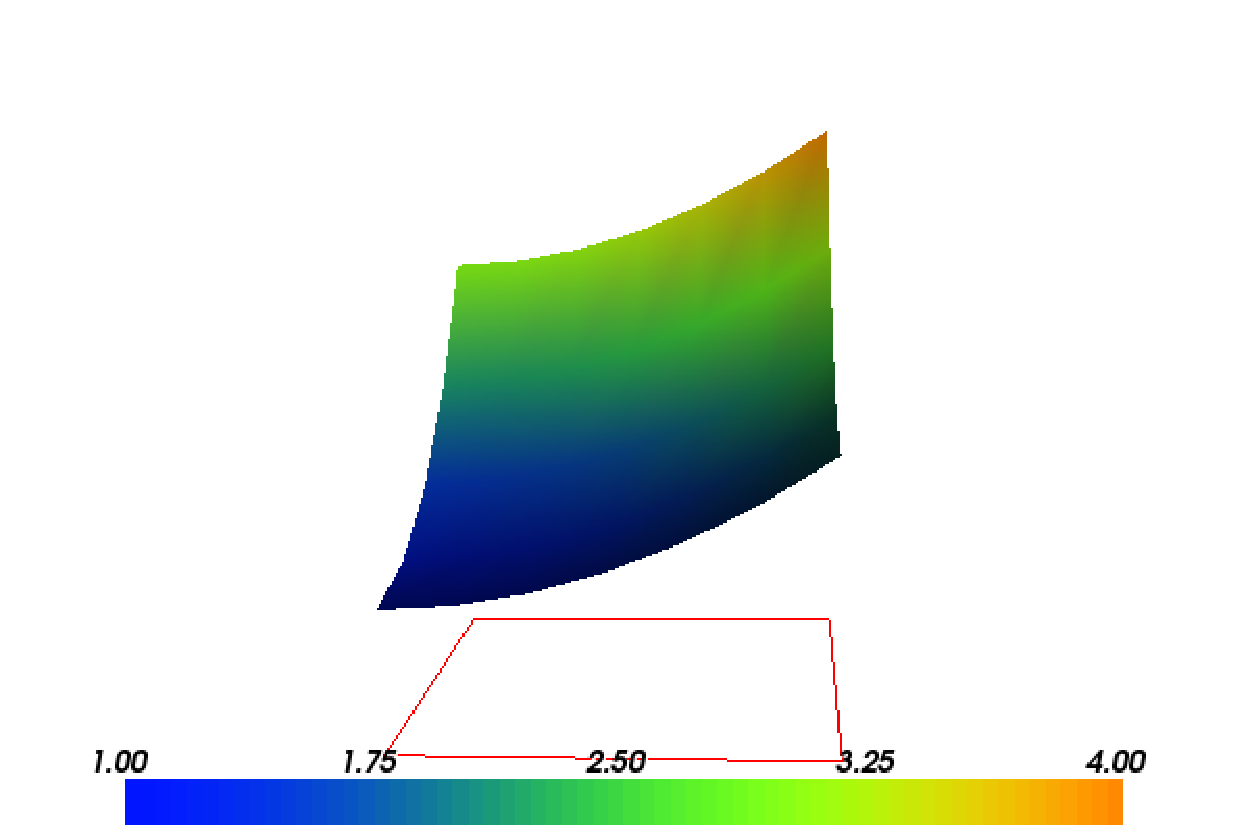
\includegraphics[width=\largefig]{chapters/langtangen/pdf/ex1_u.pdf}
  \caption{Plot of the solution in the first \fenics{} example.
    (A bounding box around the mesh is added by pressing \emp{o} in the plot
    window, and the mouse buttons are then used to rotate and move the
    plot, see Section~\ref{langtangen:quickviz}.)}
  \label{tut:poisson:2D:fig:ex1:u}
\end{figure}

\begin{figure}
  \center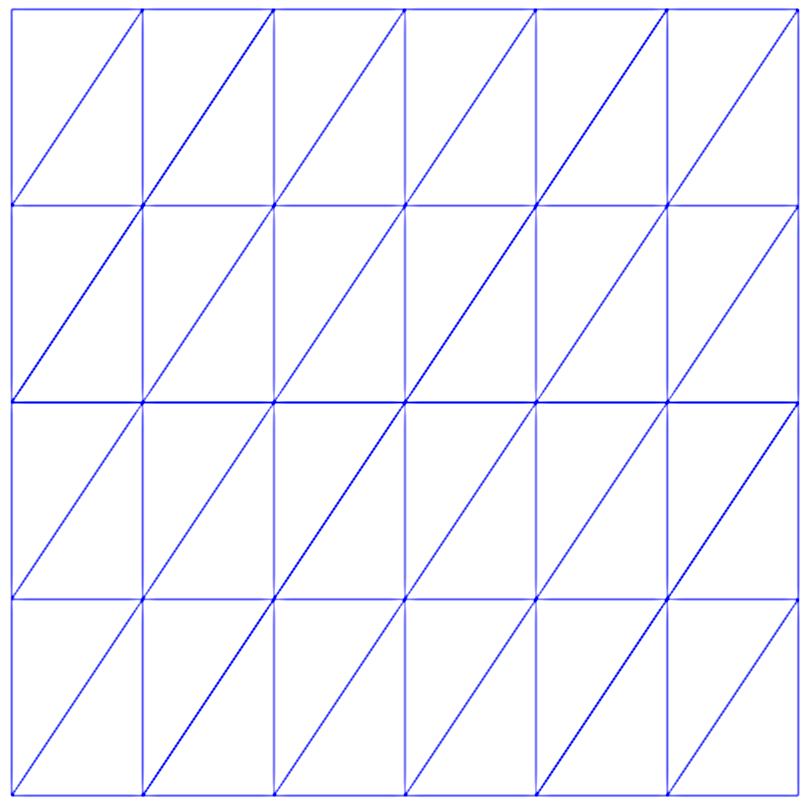
\includegraphics[width=\smallfig]{chapters/langtangen/png/ex1_mesh.png}
  \caption{Plot of the mesh in the first \fenics{} example.}
  \label{tut:poisson:2D:fig:ex1:mesh}
\end{figure}

\subsection{Examining the discrete solution}
\label{langtangen:poisson1:verify1}

We know that, in the particular boundary-value problem of
Section~\ref{langtangen:poisson1:impl}, the computed solution $u$ should
equal the exact solution at the vertices of the cells.  An important
extension of our first program is therefore to examine the computed
values of the solution, which is the focus of the present section.

A finite element function like $u$ is expressed as a linear combination
of basis functions $\phi_j$, spanning the space $V$:
\begin{equation}
  \sum_{j=1}^N U_j \phi_j.
\label{langtangen:poisson1:ufem}
\end{equation}
By writing \emp{u = problem.solve()} in the program, a linear system
will be formed from $a$ and $L$, and this system is solved for
the $U_1,\ldots,U_N$ values. The $U_1,\ldots,U_N$ values are known
\index{degree of freedom} as \emph{degrees of freedom} of $u$. For
Lagrange elements (and many other element types) $U_k$ is simply the value
of $u$ at the node with global number $k$.  (The nodes and cell vertices
coincide for linear Lagrange elements, while for higher-order elements
there may be additional nodes at the facets and in the interior of cells.)

Having \emp{u} represented as a \emp{Function} object, we can either
evaluate \emp{u(x)} at any vertex \emp{x} in the mesh, or we can grab
all the values $U_j$ directly by
\begin{python}
u_nodal_values = u.vector()
\end{python}
The result is a DOLFIN \emp{Vector} object, which is basically an
encapsulation of the vector object used in the linear algebra package
that is applied to solve the linear system arising form the variational
problem.  Since we program in Python it is convenient to convert
the \emp{Vector} object to a standard \emp{numpy} array for further
processing:\index{degrees of freedom array}\index{nodal values array}
\begin{python}
u_array = u_nodal_values.array()
\end{python}
With \emp{numpy} arrays we can write ``MATLAB-like'' code to analyze
the data. Indexing is done with square brackets: \emp{u\_array[i]},
where the index \emp{i} always starts at \emp{0}.

The coordinates of the vertices in the mesh can be extracted by
\begin{python}
coor = mesh.coordinates()
\end{python}
For a $d$-dimensional problem, \emp{coor} is an $M\times d$ \emp{numpy}
array, $M$ being the number of vertices in the mesh. Writing out the
solution on the screen can now be done by a simple loop:
\begin{python}
for i in range(len(u_array)):
    print "u(%8g,%8g) = %g" % \
          (coor[i][0], coor[i][1], u_array[i])
\end{python}
The beginning of the output looks like this:
\begin{progoutput}
u(       0,       0) = 1
u(0.166667,       0) = 1.02778
u(0.333333,       0) = 1.11111
u(     0.5,       0) = 1.25
u(0.666667,       0) = 1.44444
u(0.833333,       0) = 1.69444
u(       1,       0) = 2
\end{progoutput}
\noindent
For Lagrange elements of degree higher than one, the vertices and the
nodes do not coincide, and then the loop above is meaningless.

For verification purposes we want to compare the values of \emp{u}
at the nodes; that is, the values of the vector \emp{u\_array}, with
the exact solution given by \emp{u0}. At each node, the difference
between the computed and exact solution should be less than a small
tolerance. The exact solution is given by the \emp{Expression}
object \emp{u0}, which we can evaluate directly as \emp{u0(coor[i])}
at the vertex with global number \emp{i}, or as \emp{u0(x)} for any
spatial point.  Alternatively, we can make a finite element field
\emp{u\_e}, representing the exact solution, whose values at the
nodes are given by the \emp{u0} function. With mathematics, $u_e
= \sum_{j=1}^N E_j\phi_j$, where $E_j=u_0(x_j,y_j)$, $(x_j,y_j)$
being the coordinates of node number $j$.  This process is known as
interpolation.\index{interpolation}\index{interpolate} FEniCS
has a function for performing the operation:
\begin{python}
u_e = interpolate(u0, V)
\end{python}
The maximum error can now be computed as
\begin{python}
u_e_array = u_e.vector().array()
diff = abs(u_array - u_e_array)
print "Max error:", diff.max()

# or more compactly:
print "Max error:", abs(u_e_array - u_array).max()
\end{python}
The value of the error should be at the level of the machine precision
($10^{-16}$).

To demonstrate the use of point evaluations of \emp{Function} objects,
we write out the computed \emp{u} at the center point of the domain and
compare it with the exact solution:
\begin{python}
center = (0.5, 0.5)
u_value = u(center)
u0_value = u0(center)
print "numerical u at the center point:", u_value
print "exact     u at the center point:", u0_value
\end{python}
Trying a $3\times 3$ mesh, the output from the previous snippet becomes
\begin{progoutput}
numerical u at the center point: [ 1.83333333]
exact     u at the center point: [ 1.75]
\end{progoutput}
\noindent
The discrepancy is due to the fact that the center point is not a node in
this particular mesh, but a point in the interior of a cell, and \emp{u}
varies linearly over the cell while \emp{u0} is a quadratic function.

Mesh information can be gathered from the \emp{mesh} object, e.g.,
\begin{itemize}
  \item \emp{mesh.num\_cells()} returns the number of cells (triangles)
  in the mesh,

  \item \emp{mesh.num\_vertices()} returns the number of vertices in
  the mesh (with our choice of linear Lagrange elements this equals the
  number of nodes),

  \item \emp{str(mesh)} returns a short ``pretty print'' description of
  the mesh, e.g.,
\begin{progoutput}
<Mesh of topological dimension 2 (triangles) with
16 vertices and 18 cells, ordered>
\end{progoutput}
  \noindent
  and \emp{print mesh} is actually the same as \emp{print str(mesh)}.
\end{itemize}
All mesh objects are of type \emp{Mesh} so typing the command \emp{pydoc
dolfin.Mesh}\index{pydoc} in a terminal window will give a list
of methods\footnote{A method in Python (and other
  languages supporting the class construct) is simply a function in a
  class.} that can be called through any \emp{Mesh} object. In fact,
\emp{pydoc dolfin.X} shows the documentation of any DOLFIN name \emp{X}
(at the time of this writing, some names have missing or incomplete
documentation).

We have seen how to extract the nodal values in a \emp{numpy} array.
If desired, we can adjust the nodal values too. Say we want to normalize
the solution such that the maximum value is 1. Then we must divide all $U_j$
values by $\max\{U_1,\ldots,U_N\}$. The following snippet performs the task:
\begin{python}
max_u = u_array.max()
u_array /= max_u
u.vector()[:] = u_array
print u.vector().array()
\end{python}
That is, we manipulate \emp{u\_array} as desired, and then we insert
this array into \emp{u}'s \emp{Vector} object.  The \emp{/=} operator
implies an in-place modification of the object on the left-hand side:
all elements of the \emp{u\_array} are divided by the value \emp{max\_u}.
Alternatively, one could write \emp{u\_array =
  u\_array/max\_u}, which implies creating a new array on the
right-hand side and assigning this array to the name \emp{u\_array}.
We can equally well insert the entries of \emp{u\_array} into \emp{u}'s
\emp{numpy} array:
\begin{python}
u.vector().array()[:] = u_array
\end{python}
All the code in this subsection can be found in the file
\emp{Poisson2D\_D2.py}.
%We have commented out the \emp{plot} and \emp{interactive} calls in
%this version of the program, but if you want plotting to happen, make
%sure that \emp{interactive} is called at the very end of the program.

\subsection{Formulating a real physical problem}
\label{langtangen:poisson:membrane}

Perhaps you are not particularly amazed by viewing the simple surface
of $u$ in the test problem from Sections~\ref{langtangen:poisson1:impl}
and \ref{langtangen:poisson1:verify1}.  However, solving a real physical
problem with a more interesting and amazing solution on the screen is
only a matter of specifying a more exciting domain, boundary condition,
and/or right-hand side $f$.

One possible physical problem regards the deflection $D(x,y)$ of an
elastic circular membrane with radius $R$, subject to a localized
perpendicular pressure force, modeled as a Gaussian function.
The appropriate PDE model is
\begin{equation}
-T\Delta D = p(x,y)\quad\hbox{in }\Omega = \{ (x,y)\,|\, x^2+y^2\leqslant R\},
\end{equation}
with
\begin{equation}
p(x,y) = \frac{A}{2\pi\sigma}\exp{\left(
- \frac{1}{2}\left( \frac{x-x_0}{\sigma}\right)^2
- \frac{1}{2}\left( \frac{y-y_0}{\sigma}\right)^2
\right)}.
\end{equation}
Here, $T$ is the tension in the membrane (constant), $p$ is the
external pressure load, $A$ the amplitude of the pressure, $(x_0,y_0)$
the localization of the Gaussian pressure function, and $\sigma$ the
``width'' of this function. The boundary condition is $D=0$.

Introducing a scaling with $R$ as characteristic length and $8\pi\sigma
T/A$ as characteristic size\footnote{ Assuming $\sigma$ large enough
so that $p\approx\hbox{const} \sim A/(2\pi\sigma)$ in $\Omega$, we
can integrate an axi-symmetric version of the equation in the radial
coordinate $r\in [0,R]$ and obtain $D=(r^2-R^2)A/(8\pi\sigma T)$, which
for $r=0$ gives a rough estimate of the size of $|D|$: $AR^2/(8\pi\sigma
T)$.}
 of $D$, we can derive the equivalent
scaled problem on the unit circle,
\begin{equation}
\label{langtangen:poisson1:membrane:scaled:eq}
-\Delta w =
4\exp{\left(
- \frac{1}{2}\left( \frac{Rx-x_0}{\sigma}\right)^2
- \frac{1}{2}\left( \frac{Ry-y_0}{\sigma}\right)^2
\right)},
\end{equation}
with $w=0$ on the boundary. We have that $D = AR^2w/(8\pi\sigma T)$.

A mesh over the unit circle can be created by
\begin{python}
mesh = UnitCircle(n)
\end{python}
where \emp{n} is the typical number of elements in the radial
direction.  You should now be able to figure out how to modify the
\emp{Poisson2D\_D1.py} code to solve this membrane problem.  More
specifically, you are recommended to perform the following extensions:
\begin{enumerate}
  \item initialize $R$, $x_0$, $y_0$, $\sigma$, $T$, and $A$ in the
  beginning of the program,

  \item build a string expression for $p$ with correct C++ syntax (use
  ``printf'' formatting in Python to build the expression),

  \item define the \emp{a} and \emp{L} variables in the variational
  problem for $w$ and compute the solution,

  \item plot the mesh, $w$, and the scaled pressure function $p$ (the
  right-hand side of \eqref{langtangen:poisson1:membrane:scaled:eq}),

  \item write out the maximum real deflection $D$ (the maximum of the $w$
  values times $A/(8\pi\sigma T)$).
\end{enumerate}
Use variable names in the program similar to the mathematical symbols
in this problem.

Choosing a small width $\sigma$ (say 0.01) and a location $(x_0,y_0)$
toward the circular boundary (say $(0.6R\cos\theta, 0.6R\sin\theta)$
for any $\theta\in [0,2\pi]$), may produce an exciting visual comparison
of $w$ and $p$ that demonstrates the very smoothed elastic response to a
peak force (or mathematically, the smoothing properties of the inverse of
the Laplace operator).  You need to experiment with the mesh resolution
to get a smooth visual representation of~$p$.

In the limit $\sigma\rightarrow\infty$, the right-hand side $p$ of
\eqref{langtangen:poisson1:membrane:scaled:eq} approaches the constant
4, and then the solution should be $w(x,y) = 1-x^2-y^2$.  Compute the
absolute value of the difference between the exact and the numerical
solution if $\sigma \geqslant 50$ and write out the maximum difference
to provide some evidence that the implementation is correct.

You are strongly encouraged to spend some time on doing this exercise and
play around with the plots and different mesh resolutions.  A suggested
solution to the exercise can be found in the file \emp{membrane1.py}.

\begin{python}
from dolfin import *

# Set pressure function:
T = 10.0  # tension
A = 1.0   # pressure amplitude
R = 0.3   # radius of domain
theta = 0.2
x0 = 0.6*R*cos(theta)
y0 = 0.6*R*sin(theta)
sigma = 0.025
#sigma = 50  # verification
pressure = "4*exp(-0.5*(pow((%g*x[0] - %g)/%g, 2)) "\
           "     - 0.5*(pow((%g*x[1] - %g)/%g, 2)))" % \
           (R, x0, sigma, R, y0, sigma)

n = 40   # approx no of elements in radial direction
mesh = UnitCircle(n)
V = FunctionSpace(mesh, "Lagrange", 1)

# Define boundary condition w=0

def boundary(x, on_boundary):
    return on_boundary

bc = DirichletBC(V, Constant(0.0), boundary)

# Define variational problem
w = TrialFunction(V)
v = TestFunction(V)
p = Expression(pressure)
a = inner(grad(w), grad(v))*dx
L = v*p*dx

# Compute solution
problem = VariationalProblem(a, L, bc)
w = problem.solve()

# Plot solution and mesh
plot(mesh, title="Mesh over scaled domain")
plot(w, title="Scaled deflection")
p = interpolate(p, V)
plot(p, title="Scaled pressure")

# Find maximum real deflection
max_w = w.vector().array().max()
max_D = A*max_w/(8*pi*sigma*T)
print "Maximum real deflection is", max_D

# Verification for "flat" pressure (big sigma)
if sigma >= 50:
    w_exact = Expression("1 - x[0]*x[0] - x[1]*x[1]")
    w_e = interpolate(w_exact, V)
    w_e_array = w_e.vector().array()
    w_array = w.vector().array()
    diff_array = abs(w_e_array - w_array)
    print "Verification of the solution, max difference is %.4E" % \
          diff_array.max()

    # Create finite element field over V and fill with error values
    difference = Function(V)
    difference.vector()[:] = diff_array
    #plot(difference, title="Error field for sigma=%g" % sigma)

# Should be at the end
interactive()
\end{python}

\subsection{Computing derivatives}
\label{langtangen:poisson:gradu}

In many Poisson and other problems the gradient of the solution is of
interest. The computation is in principle simple: since $u = \sum_{j=1}^N
U_j \phi_j$, we have that
\begin{equation}
  \nabla u = \sum_{j=1}^N U_j \nabla \phi_j.
\end{equation}
Given the solution variable \emp{u} in the program, \emp{grad(u)} denotes
the gradient. However, the gradient of a piecewise continuous finite
element scalar field is a discontinuous vector field since the $\phi_j$
has discontinuous derivatives at the boundaries of the cells. For example,
using Lagrange elements of degree 1, $u$ is linear over each cell, and
the numerical $\nabla u$ becomes a piecewise constant vector field. On
the contrary, the exact gradient is continuous.  For visualization
and data analysis purposes we often want the computed gradient to be a
continuous vector field. Typically, we want each component of $\nabla
u$ to be represented in the same way as $u$ itself. To this end,
we can project the components of $\nabla u$ onto the same function
space as we used for $u$.  This means that we solve $w = \nabla u$
approximately by a finite element method\footnote{This process is known as
\emph{projection}\index{projection}.  Looking at the component $\partial
u/\partial x$ of the gradient, we project the (discrete) derivative
$\sum_jU_j{\partial \phi_j/\partial x}$ onto another function space
with basis $\bar\phi_1,\bar\phi_2,\ldots$ such that the derivative in
this space is expressed by the standard sum $\sum_j\bar U_j\bar \phi_j$,
for suitable (new) coefficients $\bar U_j$.}, using the same elements
for the components of $w$ as we used for $u$.

The variational problem for $w$ reads: find $w\in V^{(\mbox{g})}$ such that
\begin{equation}
  a(w, v) = L(v)\quad\foralls v\in \hat{V}^{(\mbox{g})},
\end{equation}
where
\begin{align}
  a(w, v) &= \int_\Omega w\cdot v\dx,
\\
  L(v) &= \int_\Omega \nabla u\cdot v\dx.
\end{align}
The function spaces $V^{(\mbox{g})}$ and $\hat{V}^{(\mbox{g})}$ (with
the superscript g denoting ``gradient'') are vector versions of the
function space for $u$, with boundary conditions removed (if $V$ is
the space we used for $u$, with no restrictions on boundary values, $
V^{(\mbox{g})} = \hat{V}^{(\mbox{g})} = [V]^d$, where $d$ is the
number of space dimensions).  For example, if we used piecewise linear
functions on the mesh to approximate $u$, the variational problem for
$w$ corresponds to approximating each component field of $w$ by
piecewise linear functions.

The variational problem for the vector field $w$, called \emp{gradu}
in the code, is easy to solve in \fenics:
\begin{python}
V_g = VectorFunctionSpace(mesh, "Lagrange", 1)
w = TrialFunction(V_g)
v = TestFunction(V_g)

a = inner(w, v)*dx
L = inner(grad(u), v)*dx
problem = VariationalProblem(a, L)
gradu = problem.solve()

plot(gradu, title="grad(u)")
\end{python}
The new thing is basically that we work with a
\emp{VectorFunctionSpace}, since the unknown is now a vector
field, instead of the \emp{FunctionSpace} object for scalar fields.
Figure~\ref{tut:poisson:2D:fig:ex1:gradu} shows an example of how Viper
can visualize such a vector field.

\begin{figure}
  \center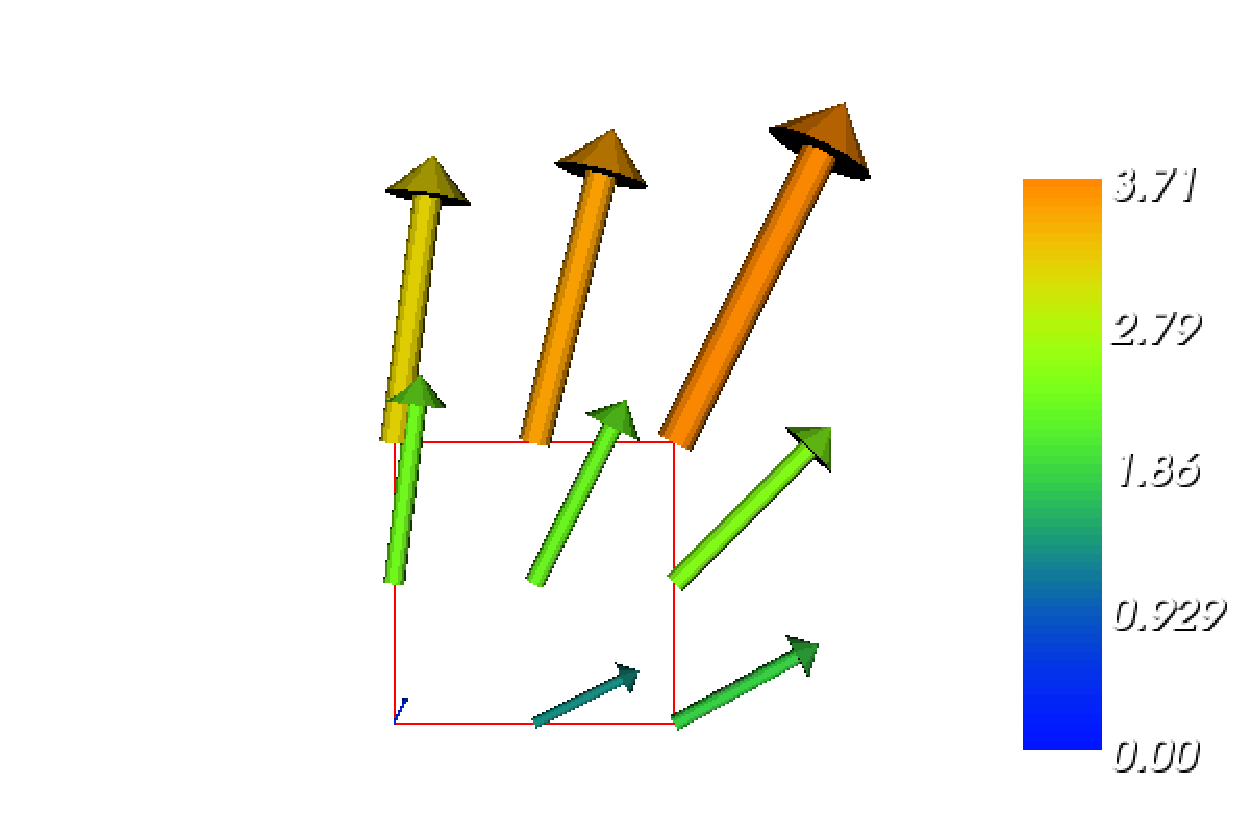
\includegraphics[width=\largefig]{chapters/langtangen/pdf/ex1_gradu.pdf}
  \caption{Example on visualizing the vector field
    $\nabla u$ by arrows at the nodes.}
  \label{tut:poisson:2D:fig:ex1:gradu}
\end{figure}

The scalar component fields of the gradient can be extracted as separate
fields and, e.g., visualized:
\begin{python}
gradu_x, gradu_y = gradu.split(deepcopy=True)  # extract components
plot(gradu_x, title="x-component of grad(u)")
plot(gradu_y, title="y-component of grad(u)")
\end{python}
The \emp{deepcopy=True} argument signifies a \emph{deep copy}, which
is a general term in computer science implying that a copy of the data
is returned. (The opposite, \emp{deepcopy=False}, means a \emph{shallow
copy}, where the returned objects are just pointers to the original data.)

The \emp{gradu\_x} and \emp{gradu\_y} variables behave as \emp{Function}
objects. In particular, we can extract the underlying arrays of nodal
values by\index{degrees of freedom array} \index{nodal values array}
\begin{python}
gradu_x_array = gradu_x.vector().array()
gradu_y_array = gradu_y.vector().array()
\end{python}
The degrees of freedom of the \emp{gradu} vector field can also be
reached by \index{degrees of freedom array!vector field}
\begin{python}
gradu_array = gradu.vector().array()
\end{python}
but this is a flat \emp{numpy} array where the degrees of freedom for
the $x$ component of the gradient is stored in the first part, then the
degrees of freedom of the $y$ component, and so on.

The program \emp{Poisson2D\_D3.py} extends the code \emp{Poisson2D\_D2.py}
from Section~\ref{langtangen:poisson1:verify1} with computations
and visualizations of the gradient.  Examining the arrays
\emp{gradu\_x\_array} and \emp{gradu\_y\_array}, or looking at the
plots of \emp{gradu\_x} and \emp{gradu\_y}, quickly reveals that the
computed \emp{gradu} field does not equal the exact gradient $(2x,
4y)$ in this particular test problem where $u=1+x^2+2y^2$.  There are
inaccuracies at the boundaries, arising from the approximation problem for
$w$. Increasing the mesh resolution shows, however, that the components
of the gradient vary linearly as $2x$ and $4y$ in the interior of
the mesh (as soon as we are one element away from the boundary). See
Section~\ref{langtangen:quickviz} for illustrations of this phenomenon.

Representing the gradient by the same elements as we used for the solution
is a very common step in finite element programs, so the formation and
solution of a variational problem for $w$ as shown above can be replaced
by a one-line call:\index{project}\index{projection}
\begin{python}
gradu = project(grad(u), VectorFunctionSpace(mesh, "Lagrange", 1))
\end{python}
The \emp{project} function can take an expression involving some finite
element function in some space and project the expression onto another
space.  The applications are many, including turning discontinuous
gradient fields into continuous ones, comparing higher- and lower-order
function approximations, and transforming a higher-order finite element
solution down to a piecewise linear field, which is required by many
visualization packages.

\subsection{Computing functionals}
\label{langtangen:poisson1:functionals}
\index{functionals}

After the solution $u$ of a PDE is computed, we often want to compute
functionals of $u$, for example,
\begin{equation}
  \frac{1}{2} ||\nabla u||^2 \equiv \frac{1}{2}\int_\Omega \nabla u\cdot \nabla u\dx,
\label{langtangen:poisson1:functionals:energy}
\end{equation}
which often reflects some energy quantity.  Another frequently
occurring functional is the error
\begin{equation}
  ||u_e-u|| = \left(\int_\Omega (u_e-u)^2\dx\right)^{1/2},
\label{langtangen:poisson1:functionals:error}
\end{equation}
which is of particular interest when studying convergence properties.
Sometimes the interest concerns the flux out of a part $\Gamma$ of the
boundary $\partial\Omega$,
\begin{equation}
  F = -\int_\Gamma p\nabla u\cdot  \ds,
\label{langtangen:poisson1:functionals:flux}
\end{equation}
where $n$ is an outward unit normal
at $\Gamma$ and $p$ is a coefficient (see the problem in
Section~\ref{langtangen:possion:2D:varcoeff} for a specific example).
All these functionals are easy to compute with \fenics, and this section
describes how it can be done.

\paragraph{Energy functional.}\index{energy functional}
The integrand of the energy functional
\eqref{langtangen:poisson1:functionals:energy} is described in the UFL
language in the same manner as we describe weak forms:
\begin{python}
energy = 0.5*inner(grad(u), grad(u))*dx
E = assemble(energy)
\end{python}
The \emp{assemble} call performs the integration.  It is possible to
restrict the integration to subdomains, or parts of the boundary,
by using a mesh function to mark the subdomains (this technique will be
explained
in Section~\ref{langtangen:poisson:mat:neumann}).  The program
\emp{membrane2.py} carries out the computation of the elastic energy
\begin{equation}
   \frac{1}{2}||T\nabla D||^2 = \frac{1}{2}\left(\frac{AR}{8\pi\sigma}\right)^2
    ||\nabla w||^2
\end{equation}
in the membrane problem from Section~\ref{langtangen:poisson:membrane}.

\paragraph{Convergence estimation.}\index{error functional}
To illustrate error computations and convergence of finite element
solutions, we modify the \emp{Poisson2D\_D3.py} program from
Section~\ref{langtangen:poisson:gradu} and specify a more complicated
solution,
\begin{equation}
   u(x,y) = \sin(\omega\pi x)\sin(\omega\pi y)
\end{equation}
on the unit square.  This choice implies $f(x,y)=2\omega^2\pi^2 u(x,y)$.
With $\omega$ restricted to an integer it follows that $u_0=0$. We must
define the appropriate boundary conditions, the exact solution, and the
$f$ function in the code:
\begin{python}
def boundary(x, on_boundary):
    return on_boundary

bc = DirichletBC(V, Constant(0.0), boundary)

omega = 1.0
u_exact = Expression("sin(%g*pi*x[0])*sin(%g*pi*x[1])" % \
                     (omega, omega))

f = 2*pi**2*omega**2*u_exact
\end{python}

The computation of \eqref{langtangen:poisson1:functionals:error} can be
done by
\begin{python}
error = (u - u_exact)**2*dx
E = sqrt(assemble(error))
\end{python}
However, \emp{u\_exact} will here be interpolated onto the function
space \emp{V}; that is, the exact solution used in the integral will
vary linearly over the cells, and not as a sine function, if \emp{V}
corresponds to linear Lagrange elements.  This may yield a smaller error
\emp{u - u\_e} than what is actually true.

More accurate representation of the exact solution is easily achieved by
interpolating the formula onto a space defined by higher-order elements,
say of third degree:
\begin{python}
Ve = FunctionSpace(mesh, "Lagrange", degree=3)
u_e = interpolate(u_exact, Ve)
error = (u - u_e)**2*dx
E = sqrt(assemble(error))
\end{python}
The \emp{u} function will here be automatically interpolated and
represented in the \emp{Ve} space. When functions in different function
spaces enter UFL expressions, they will be represented in the space
of highest order before integrations are carried out. When in doubt,
we should explicitly interpolate \emp{u}:
\begin{python}
u_Ve = interpolate(u, Ve)
error = (u_Ve - u_e)**2*dx
\end{python}

The square in the expression for \emp{error} will be expanded and lead
to a lot of terms that almost cancel when the error is small, with the
potential of introducing significant round-off errors.  The function
\emp{errornorm} is available for avoiding this effect by first
interpolating \emp{u} and \emp{u\_exact} to a space with higher-order
elements, then subtracting the degrees of freedom, and then performing
the integration of the error field. The usage is simple:
\begin{python}
  E = errornorm(u_exact, u, normtype="L2", degree=3)
\end{python}
At the time of this writing, \emp{errornorm} does not work with
\emp{Expression} objects for \emp{u\_exact}, making the function
inapplicable for most practical purposes. Nevertheless, we can easily
express the procedure explicitly:
\begin{python}
def errornorm(u_exact, u, Ve):
    u_Ve = interpolate(u, Ve)
    u_e_Ve = interpolate(u_exact, Ve)
    e_Ve = Function(Ve)
    # Subtract degrees of freedom for the error field
    e_Ve.vector()[:] = u_e_Ve.vector().array() - \
                       u_Ve.vector().array()
    error = e_Ve**2*dx
    return sqrt(assemble(error))
\end{python}
The \emp{errornorm} procedure turns out to be identical to computing
the expression \emp{(u\_e - u)**2*dx} directly in the present test case.

Sometimes it is of interest to compute the error of the gradient field:
$||\nabla (u-u_e)||$ (often referred to as the $H^1$ seminorm of the
error).  Given the error field \emp{e\_Ve} above, we simply write
\begin{python}
  H1seminorm = sqrt(assemble(inner(grad(e_Ve), grad(e_Ve))*dx))
\end{python}

Finally, we remove all \emp{plot} calls and printouts of $u$ values in
the original program, and collect the computations in a function:
\begin{python}
def compute(nx, ny, polynomial_degree):
    mesh = UnitSquare(nx, ny)
    V = FunctionSpace(mesh, "Lagrange", degree=polynomial_degree)
    ...
    Ve = FunctionSpace(mesh, "Lagrange", degree=3)
    E = errornorm(u_exact, u, Ve)
    return E
\end{python}

Calling \emp{compute} for finer and finer meshes enables us to study
the convergence rate. Define the element size $h=1/n$, where $n$ is the
number of divisions in $x$ and $y$ direction (\emp{nx=ny} in the code). We
perform experiments with $h_0>h_1>h_2\cdots$ and compute the corresponding
errors $E_0, E_1, E_3$ and so forth.  Assuming $E_i=Ch_i^r$ for unknown
constants $C$ and $r$, we can compare two consecutive experiments,
$E_i=Ch_i^r$ and $E_{i-1}=Ch_{i-1}^r$, and solve for $r$:
\begin{equation}
  r = \frac{\ln(E_i/E_{i-1})}{\ln (h_i/h_{i-1})}.
\end{equation}
The $r$ values should approach the expected convergence rate
\emp{degree+1} as $i$ increases.

The procedure above can easily be turned into Python code:
\begin{python}
import sys
degree = int(sys.argv[1])  # read degree as 1st command-line arg
h = []  # element sizes
E = []  # errors
for nx in [4, 8, 16, 32, 64, 128, 264]:
    h.append(1.0/nx)
    E.append(compute(nx, nx, degree))

# Convergence rates
from math import log as ln  # (log is a dolfin name too)
for i in range(1, len(E)):
    r = ln(E[i]/E[i-1])/ln(h[i]/h[i-1])
    print "h=%10.2E r=%.2f" % (h[i], r)
\end{python}
The resulting program has the name \emp{Poisson2D\_D4.py} and computes
error norms in various ways. Running this program for elements of first
degree and $\omega=1$ yields the output
\begin{progoutput}
h=1.25E-01 E=3.25E-02 r=1.83
h=6.25E-02 E=8.37E-03 r=1.96
h=3.12E-02 E=2.11E-03 r=1.99
h=1.56E-02 E=5.29E-04 r=2.00
h=7.81E-03 E=1.32E-04 r=2.00
h=3.79E-03 E=3.11E-05 r=2.00
\end{progoutput}
\noindent
That is, we approach the expected second-order convergence of linear
Lagrange elements as the meshes become sufficiently fine.

Running the program for second-degree elements results in the expected
value $r=3$,
\begin{progoutput}
h=1.25E-01 E=5.66E-04 r=3.09
h=6.25E-02 E=6.93E-05 r=3.03
h=3.12E-02 E=8.62E-06 r=3.01
h=1.56E-02 E=1.08E-06 r=3.00
h=7.81E-03 E=1.34E-07 r=3.00
h=3.79E-03 E=1.53E-08 r=3.00
\end{progoutput}
\noindent
However, using \emp{(u - u\_exact)**2} for the error computation, which
implies interpolating \emp{u\_exact} onto the same space as \emp{u},
results in $r=4$ (!). This is an example where it is important to
interpolate \emp{u\_exact} to a higher-order space (polynomials of
degree 3 are sufficient here) to avoid computing a too optimistic
convergence rate.
%Looking at the error in the degrees of freedom
%(\emp{u.vector().array()}) reveals a convergence rate of $r=4$ for
%second-degree elements. For elements of polynomial degree 3 all the rates
%are $r=4$, regardless of whether we choose a ``fine'' space \emp{Ve}
%with polynomials of degree 3 or~5.

Running the program for third-degree elements results in the expected
value~$r=4$:
\begin{progoutput}
h=1.25E-01 r=4.09
h=6.25E-02 r=4.03
h=3.12E-02 r=4.01
h=1.56E-02 r=4.00
h=7.81E-03 r=4.00
\end{progoutput}
\noindent
Checking convergence rates is the next best method for verifying
PDE codes (the best being exact recovery of a solution as in
Section~\ref{langtangen:poisson1:verify1} and many other places in
this tutorial).

\paragraph{Flux functionals.}\index{flux functional}
To compute flux integrals like
\eqref{langtangen:poisson1:functionals:flux} we need to define the
$n$ vector, referred to as \emph{facet normal} in
\fenics. If $\Gamma$ is the complete boundary we can perform the flux
computation by
\begin{python}
n = FacetNormal(mesh)
flux = -p*inner(grad(u), n)*ds
total_flux = assemble(flux)
\end{python}
It is possible to restrict the integration to a part of the boundary
using a mesh function to mark the relevant part, as explained in
Section~\ref{langtangen:poisson:mat:neumann}. Assuming that the part
corresponds to subdomain number \emp{n}, the relevant form for the flux
is \emp{-p*inner(grad(u), n)*ds(n)}.

\subsection{Quick visualization with VTK}
\label{langtangen:quickviz}
\index{visualization}\index{Viper}\index{VTK}

As we go along with examples it is fun to play around with \emp{plot}
commands and visualize what is computed. This section explains some
useful visualization features.

The \emp{plot(u)} command launches a \fenics{} component called Viper,
which applies the VTK package to visualize finite element functions.
Viper is not a full-fledged, easy-to-use front-end to VTK (like ParaView
or VisIt), but rather a thin layer on top of VTK's Python interface,
allowing us to quickly visualize a DOLFIN function or mesh, or data
in plain Numerical Python arrays, within a Python program.  Viper is
ideal for debugging, teaching, and initial scientific investigations.
The visualization can be interactive, or you can steer and automate it
through program statements.  More advanced and professional visualizations
are usually better done with advanced tools like MayaVi2, ParaView,
or VisIt.

We have made a program \emp{membrane1v.py} for the membrane deflection
problem in Section~\ref{langtangen:poisson:membrane} and added various
demonstrations of Viper capabilities. You are encouraged to play around
with \emp{membrane1v.py} and modify the code as you read about various
features.  The \emp{membrane1v.py} program solves the two-dimensional
Poisson equation for a scalar field \emp{w} (the membrane deflection).

The \emp{plot} function can take additional arguments, such as a title
of the plot, or a specification of a wireframe plot (elevated mesh)
instead of a colored surface plot:\index{plot}
\begin{python}
plot(mesh, title="Finite element mesh")
plot(w, wireframe=True, title="solution")
\end{python}

The three mouse buttons can be used to rotate, translate, and zoom
the surface.  Pressing \emp{h} in the plot window makes a printout of
several key bindings that are available in such windows. For example,
pressing \emp{m} in the mesh plot window dumps the plot of the mesh to an
Encapsulated PostScript (\emp{.eps}) file, while pressing \emp{i} saves
the plot in PNG format.  All file names are automatically generated as
\emp{simulationX.eps}, where \emp{X} is a counter \emp{0000}, \emp{0001},
\emp{0002}, etc., being increased every time a new plot file in that
format is generated (the extension of PNG files is \emp{.png} instead
of \emp{.eps}).  Pressing \emp{o} adds a red outline of a bounding box
around the domain.

One can alternatively control the visualization from the program code
directly. This is done through a \emp{Viper} object returned from the
\emp{plot} command. Let us grab this object and use it to 1) tilt the
camera $-65$ degrees in latitude direction, 2) add $x$ and $y$ axes, 3)
change the default name of the plot files (generated by typing \emp{m}
and \emp{i} in the plot window), 4) change the color scale, and 5)
write the plot to a PNG and an EPS file. Here is the code:
\begin{python}
viz_w = plot(w,
            wireframe=False,
            title="Scaled membrane deflection",
            rescale=False,
            axes=True,              # include axes
            basename="deflection",  # default plotfile name
            )

viz_w.elevate(-65) # tilt camera -65 degrees (latitude dir)
viz_w.set_min_max(0, 0.5*max_w)  # color scale
viz_w.update(w)    # bring settings above into action
viz_w.write_png("deflection.png")
viz_w.write_ps("deflection", format="eps")
\end{python}
The \emp{format} argument in the latter line can also take the values
\emp{"ps"} for a standard PostScript file and \emp{"pdf"} for a PDF file.
Note the necessity of the \emp{viz\_w.update(w)} call -- without it we
will not see the effects of tilting the camera and changing the color
scale. Figure~\ref{langtangen:poisson:2D:fig1} shows the resulting
scalar surface.
\begin{figure}
  \center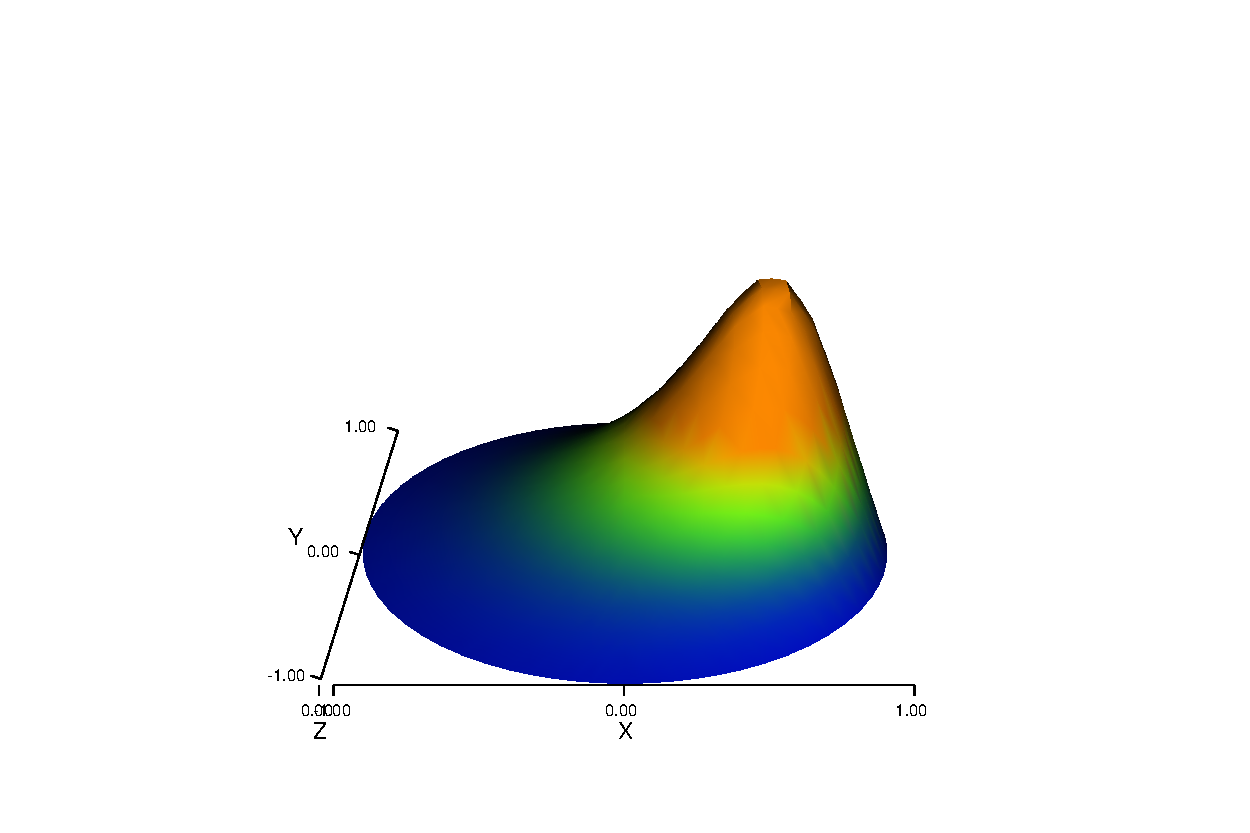
\includegraphics[width=\largefig]{chapters/langtangen/pdf/membrane_waxis.pdf}
  \caption{Plot of the deflection of a membrane.}
  \label{langtangen:poisson:2D:fig1}
\end{figure}

\subsection{Combining Dirichlet and Neumann conditions}
\label{langtangen:poisson1:DN}

Let us make a slight extension of our two-dimensional Poisson problem
from Section~\ref{langtangen:poisson1:bvp} and add a Neumann boundary
condition. The domain is still the unit square, but now we set the
Dirichlet condition $u=u_0$ at the left and right sides, $x=0$ and $x=1$,
while the Neumann condition
%%
\begin{equation}
 - \frac{\partial u}{\partial n} = g
\end{equation}
%%
is applied to the remaining sides $y=0$ and $y=1$.  The Neumann condition
is also known as a \emph{natural boundary condition} (in contrast to an
essential boundary condition).  \index{Neumann boundary conditions}

Let $\Gamma_D$ and $\Gamma_N$ denote the parts of $\partial\Omega$ where
the Dirichlet and Neumann conditions apply, respectively.  The complete
boundary-value problem can be written as
\begin{align}
  -\Delta u &= f \mbox{ in } \Omega,
\\
  u &= u_0 \mbox{ on } \Gamma_D,
\\
  -\frac{\partial u}{\partial n} &= g \mbox{ on } \Gamma_N.
\end{align}
Again we choose $u=1+x^2 + 2y^2$ as the exact solution and adjust $f$,
$g$, and $u_0$ accordingly:
\begin{align}
f &= -6,
\\
g &= \left\lbrace\begin{array}{ll}
-4, & y=1\\
0,  & y=0
\end{array}\right.
\\
u_0 &= 1 + x^2 + 2y^2.
\end{align}
For ease of programming we may introduce a $g$ function defined over
the whole of $\Omega$ such that $g$ takes on the right values at $y=0$
and $y=1$. One possible extension is
\begin{equation}
   g(x,y) = -4y.
\end{equation}

The first task is to derive the variational problem. This time we cannot
omit the boundary term arising from the integration by parts, because $v$
is only zero on $\Gamma_D$. We have
\begin{equation}
 -\int_\Omega (\Delta u)v \dx
= \int_\Omega\nabla u\cdot\nabla v\dx
  - \int_{\partial\Omega} \frac{\partial u}{\partial n}v\ds,
\end{equation}
and since $v=0$ on $\Gamma_D$,
\begin{equation}
- \int_{\partial\Omega} \frac{\partial u}{\partial n}v\ds
=
- \int_{\Gamma_N} \frac{\partial u}{\partial n}v\ds
= \int_{\Gamma_N}gv\ds,
\end{equation}
by applying the boundary condition on $\Gamma_N$.  The resulting weak
form reads
\begin{equation}
\int_{\Omega} \nabla u \cdot \nabla v \dx +
\int_{\Gamma_N} gv\ds
= \int_{\Omega} fv \dx.
\label{langtangen:poisson:2D:DN:weak}
\end{equation}
Expressing \eqref{langtangen:poisson:2D:DN:weak} in the standard notation
$a(u,v)=L(v)$ is straightforward with
\begin{align}
  a(u, v) &= \int_{\Omega} \nabla u \cdot \nabla v \dx,
  \label{langtangen:poisson2:vard:a}
\\
  L(v) &= \int_{\Omega} fv \dx - \int_{\Gamma_N} gv\ds.
  \label{langtangen:poisson2:vard:L}
\end{align}

How does the Neumann condition impact the implementation?  The code
in the file \emp{Poisson2D\_D2.py} remains almost the same.  Only two
adjustments are necessary:
\begin{enumerate}
  \item The function describing the boundary where Dirichlet conditions
  apply must be modified.

  \item The new boundary term must be added to the expression in \emp{L}.
\end{enumerate}
Step 1 can be coded as
\begin{python}
def Dirichlet_boundary(x, on_boundary):
    if on_boundary:
        if x[0] == 0 or x[0] == 1:
            return True
        else:
            return False
    else:
        return False
\end{python}
A more compact implementation reads
\begin{python}
def Dirichlet_boundary(x, on_boundary):
    return on_boundary and (x[0] == 0 or x[0] == 1)
\end{python}
As pointed out already in Section~\ref{langtangen:poisson1:impl}, testing
for an exact match of real numbers is not good programming practice so
we introduce a tolerance in the test:
\begin{python}
def Dirichlet_boundary(x, on_boundary):
    tol = 1E-14   # tolerance for coordinate comparisons
    return on_boundary and \
           (abs(x[0]) < tol or abs(x[0] - 1) < tol)
\end{python}
We may also split the boundary functions into two separate pieces,
one for each part of the boundary:
\begin{python}
tol = 1E-14
def Dirichlet_boundary0(x, on_boundary):
    return on_boundary and abs(x[0]) < tol

def Dirichlet_boundary1(x, on_boundary):
    return on_boundary and abs(x[0] - 1) < tol

bc0 = DirichletBC(V, Constant(0), Dirichlet_boundary0)
bc1 = DirichletBC(V, Constant(1), Dirichlet_boundary1)
bc = [bc0, bc1]
\end{python}

The second adjustment of our program concerns the definition of \emp{L},
where we have to add a boundary integral and a definition of the $g$
function to be integrated:
\begin{python}
g = Expression("-4*x[1]")
L = f*v*dx - g*v*ds
\end{python}
The \emp{ds} variable implies a boundary integral, while \emp{dx}
implies an integral over the domain $\Omega$.  No more modifications
are necessary. Running the resulting program, found in the file
\emp{Poisson2D\_DN1.py}, shows a successful verification -- $u$ equals the
exact solution at all the nodes, regardless of how many elements we use.

\subsection{Multiple Dirichlet conditions}
\label{langtangen:poisson:multiple:Dirichlet}

The PDE problem from the previous section applies a function $u_0(x,y)$
for setting Dirichlet conditions at two parts of the boundary.
Having a single function to set multiple Dirichlet conditions is seldom
possible. The more general case is to have $m$ functions for setting
Dirichlet conditions on $m$ parts of the boundary. The purpose of this
section is to explain how such multiple conditions are treated in FEniCS
programs.

Let us return to the case from Section~\ref{langtangen:poisson1:DN}
and define two separate functions for the two Dirichlet conditions:
\begin{align}
  - \Delta u &= -6 \mbox{ in } \Omega,
\\
  u &= u_L \mbox{ on } \Gamma_0,
\\
  u &= u_R \mbox{ on } \Gamma_1,
\\
  - \frac{\partial u}{\partial n} &= g \mbox{ on } \Gamma_N.
\end{align}
Here, $\Gamma_0$ is the boundary $x=0$, while $\Gamma_1$ corresponds to
the boundary $x=1$.  We have that $u_L = 1 + 2y^2$, $u_R = 2 + 2y^2$,
and $g=-4y$.  For the left boundary $\Gamma_0$ we define the usual
triple of a function for the boundary value, a function for defining
the boundary of interest, and a \emp{DirichletBC} object:
\begin{python}
u_L = Expression("1 + 2*x[1]*x[1]")

def left_boundary(x, on_nboundary):
    tol = 1E-14   # tolerance for coordinate comparisons
    return on_boundary and abs(x[0]) < tol

Gamma_0 = DirichletBC(V, u_L, left_boundary)
\end{python}

For the boundary $x=1$ we define a similar code:
\begin{python}
u_R = Expression("2 + 2*x[1]*x[1]")

def right_boundary(x, on_boundary):
    tol = 1E-14   # tolerance for coordinate comparisons
    return on_boundary and abs(x[0] - 1) < tol

Gamma_1 = DirichletBC(V, u_R, right_boundary)
\end{python}
The various essential conditions are then collected in a list and passed
onto our problem object of type \emp{VariationalProblem}:
\begin{python}
bc = [Gamma_0, Gamma_1]
...
problem = VariationalProblem(a, L, bc)
\end{python}

If the $u$ values are constant at a part of the boundary, we may use a
simple \emp{Constant} object instead of an \emp{Expression} object.

The file \emp{Poisson2D\_DN2.py} contains a complete program which
demonstrates the constructions above.  An extended example with multiple
Neumann conditions would have been quite natural now, but this requires
marking various parts of the boundary using the mesh function concept
and is therefore left to Section~\ref{langtangen:poisson:mat:neumann}.

\subsection{A linear algebra formulation}
\label{langtangen:poisson1:linalg}

Given $a(u,v)=L(v)$, the discrete solution $u$ is computed by
inserting $u=\sum_{j=1}^N U_j \phi_j$ into $a(u,v)$ and demanding
$a(u,v)=L(v)$ to be fulfilled for $N$ test functions
$\hat\phi_1,\ldots,\hat\phi_N$. This implies
\begin{equation}
 \sum_{j=1}^N a(\phi_j,\hat\phi_i) U_j = L(\hat\phi_i),\quad i=1,\ldots,N,
\end{equation}
which is nothing but a linear system,
\begin{equation}
  AU = b,
\end{equation}
where the entries in $A$ and $b$ are given by
\begin{equation}
\begin{split}
  A_{ij} &= a(\phi_j, \hat{\phi}_i), \\
  b_i &= L(\hat\phi_i).
\end{split}
\end{equation}

The examples so far have constructed a \emp{VariationalProblem} object
and called its \emp{solve} method to compute the solution \emp{u}.
The \emp{VariationalProblem} object creates a linear system $AU=b$ and
calls an appropriate solution method for such systems.  An alternative
is dropping the use of a \emp{VariationalProblem} object and instead
asking \fenics{} to create the matrix $A$ and right-hand side $b$,
and then solve for the solution vector $U$ of the linear system.
The relevant statements read\index{assemble}\index{linear systems
(in FEniCS)}\index{assembly of linear systems}
\begin{python}
A = assemble(a)
b = assemble(L)
bc.apply(A, b)
u = Function(V)
solve(A, u.vector(), b)
\end{python}
The variables \emp{a} and \emp{L} are as before; that is, \emp{a}
refers to the bilinear form involving a \emp{TrialFunction} object
(say \emp{u}) and a \emp{TestFunction} object (\emp{v}), and \emp{L}
involves a \emp{TestFunction} object (\emp{v}). From \emp{a} and \emp{L},
the \emp{assemble} function can compute the matrix elements $A_{i,j}$
and the vector elements~$b_i$.

The matrix $A$ and vector $b$ are first assembled without
incorporating essential (Dirichlet) boundary conditions. Thereafter,
the \emp{bc.apply(A, b)} call performs the necessary modifications to
the linear system. The first three statements above can alternatively
be carried out by\footnote{The
  essential boundary conditions are now applied to the element matrices
  and vectors prior to assembly.}
\index{assemble\_system}
\begin{python}
A, b = assemble_system(a, L, bc)
\end{python}

When we have multiple Dirichlet conditions stored in a list \emp{bc},
as explained in Section~\ref{langtangen:poisson:multiple:Dirichlet},
we must apply each condition in \emp{bc} to the system:
\begin{python}
# bc is a list of DirichletBC objects
for condition in bc:
    condition.apply(A, b)
\end{python}
Alternatively, we can make the call
\begin{python}
A, b = assemble_system(a, L, bc)
\end{python}
The \emp{assemble\_system} function incorporates the boundary conditions
in a symmetric way in the coefficient matrix. (For each degree of freedom
that is known, the corresponding row and column is zeroed out and 1 is
placed on the main diagonal, and the right-hand side \emp{b} is modified
by subtracting the column in \emp{A} times the value of the degree of
freedom, and then the corresponding entry in \emp{b} is replaced by the
known value of the degree of freedom.) With \emp{condition.apply(A,
b)}, the matrix \emp{A} is modified in an unsymmetric way. (The row
is zeroed out and 1 is placed on the main diagonal, and the degree of
freedom value is inserted in \emp{b}.)

Note that the solution \emp{u} is, as before, a \emp{Function} object.
The degrees of freedom, $U=A^{-1}b$, are filled into \emp{u}'s
\emp{Vector} object (\emp{u.vector()}) by the \emp{solve} function.

The object \emp{A} is of type \emp{Matrix}, while \emp{b} and
\emp{u.vector()} are of type \emp{Vector}. We may convert the matrix and
vector data to \emp{numpy} arrays by calling the \emp{array()} method
as shown before. If you wonder how essential boundary conditions are
incorporated in the linear system, you can print out \emp{A} and \emp{b}
before and after the \emp{bc.apply(A, b)} call:
\begin{python}
if mesh.num_cells() < 16:  # print for small meshes only
    print A.array()
    print b.array()
bc.apply(A, b)
if mesh.num_cells() < 16:
    print A.array()
    print b.array()
\end{python}

With access to the elements in \emp{A} as a \emp{numpy} array we can easily
do computations on this matrix, such as computing the eigenvalues
(using the \emp{numpy.linalg.eig} function). We can alternatively dump
the matrix to file in MATLAB format and invoke MATLAB or Octave to
perform computations:
\index{\emp{File}}
\begin{python}
mfile = File("A.m"); mfile << A
\end{python}
The data files \emp{A.m} and \emp{b.m} can be loaded directly into MATLAB
or Octave. The file extension \emp{.m} ensures that \emp{A}
is dumped to file in MATLAB format.

Matrix processing in Python or MATLAB/Octave is only feasible for
small PDE problems since the \emp{numpy} arrays or matrices in MATLAB
file format are dense matrices. DOLFIN also has an interface to the
eigensolver package SLEPc, which is a preferred tool for computing the
eigenvalues of large, sparse matrices of the type encountered in PDE
problems (see \emp{demo/la/eigenvalue} in the DOLFIN source code tree for
a demo).


The complete code where our Poisson problem is solved by forming
the linear system $AU=b$ explicitly, is stored in the files
\emp{Poisson2D\_DN\_la1.py} (one common Dirichlet condition) and
\emp{Poisson2D\_DN\_la2.py} (two separate Dirichlet conditions).

Creating the linear system explicitly in a program, as an
alternative to using a \emp{VariationalProblem} object, can have some
advantages in more advanced problem settings. For example, $A$ may
be constant throughout a time-dependent simulation, so we can avoid
recalculating $A$ at every time level and save a significant amount
of simulation time.  Sections~\ref{langtangen:timedep:diffusion1:impl}
and \ref{langtangen:timedep:diffusion1:noassemble} deal with this topic
in detail.

%In other problems, we may divide the variational
%problem and linear system into different terms, say $A=M + {\dt} K$,
%where $M$ is a matrix arising from a term like $\partial u/\partial t$,
%$K$ is a term corresponding to a Laplace operator, and ${\dt}$ is
%a time discretization parameter. When ${\dt}$ is changed in time,
%we can efficiently recompute $A = M + {\dt} K$ without
%reassembling the constant matrices $M$ and $K$. This strategy may
%speed up simulations significantly.

\subsection{A variable-coefficient Poisson problem}
\label{langtangen:possion:2D:varcoeff}
\index{Poisson's equation with variable coefficient}

Suppose we have a variable coefficient $p(x,y)$ in the Laplace operator,
as in the boundary-value problem
\begin{equation} \label{langtangen:poisson:2D:varcoeff}
  \begin{split}
    - \nabla\cdot \left\lbrack
p(x,y)\nabla u(x,y)\right\rbrack &= f(x,y) \quad \mbox{in } \Omega,
    \\
    u(x,y) &= u_0(x,y) \quad \mbox{on}\  \partial\Omega.
  \end{split}
\end{equation}
We shall quickly demonstrate that this simple extension of our model
problem only requires an equally simple extension of the \fenics{} program.

Let us continue to use our favorite solution $u(x,y)=1+x^2+2y^2$ and
then prescribe $p(x,y)=x+y$. It follows that $u_0(x,y) = 1 + x^2 + 2y^2$
and $f(x,y)=-8x-10y$.

What are the modifications we need to do in the \emp{Poisson2D\_D2.py}
program from Section~\ref{langtangen:poisson1:verify1}?
\begin{enumerate}
  \item \emp{f} must be an \emp{Expression} since it is no longer
  a constant,

  \item a new \emp{Expression} \emp{p} must be defined for the variable
  coefficient,

  \item the variational problem is slightly changed.
\end{enumerate}
First we address the modified variational problem. Multiplying the PDE
in \eqref{langtangen:poisson:2D:varcoeff} and integrating by parts now
results in
%
\begin{equation}
  \int_\Omega p\nabla u\cdot\nabla v\dx -
  \int_{\partial\Omega} p \frac{\partial u}{\partial n}v\ds = \int_\Omega
  fv\dx.
\end{equation}
%
The function spaces for $u$ and $v$ are the same as in
Section~\ref{langtangen:poisson1:varform}, implying that the boundary
integral vanishes since $v=0$ on $\partial\Omega$ where we have Dirichlet
conditions.  The weak form $a(u,v)=L(v)$ then has
\begin{align}
  a(u,v) &= \int_\Omega p\nabla u\cdot\nabla v\dx,
\\
  L(v) &= \int_\Omega fv\dx.
\end{align}
In the code from Section~\ref{langtangen:poisson1:impl} we must replace
\begin{python}
a = inner(grad(u), grad(v))*dx
\end{python}
by
\begin{python}
a = p*inner(grad(u), grad(v))*dx
\end{python}
The definitions of \emp{p} and \emp{f} read
\begin{python}
p = Expression("x[0] + x[1]")
f = Expression("-8*x[0] - 10*x[1]")
\end{python}
No additional modifications are necessary. The complete code can be
found in in the file \emp{Poisson2D\_Dvc.py}. You can run it and confirm
that it recovers the exact $u$ at the nodes.

The flux $-p\nabla u$ may be of particular interest in
variable-coefficient Poisson problems. As explained in
Section~\ref{langtangen:poisson:gradu}, we normally want the piecewise
discontinuous flux or gradient to be approximated by a continuous
vector field, using the same elements as used for the numerical
solution $u$. The approximation now consists of solving $w = -p\nabla
u$ by a finite element method: find $w\in V^{(\mbox{g})}$ such that
\begin{equation}
a(w, v) = L(v)\quad\foralls v\in \hat{V}^{(\mbox{g})},
\end{equation}
where
\begin{align}
a(w, v) &= \int_\Omega w\cdot v\dx,
\\
L(v) &= \int_\Omega (-p \nabla u)\cdot v\dx.
\end{align}
This problem is identical to the one in Section~\ref{langtangen:poisson:gradu},
except that $p$ enters the integral in $L$.

The relevant Python statements for computing the flux field take the form
\begin{python}
V_g = VectorFunctionSpace(mesh, "Lagrange", 1)
w = TrialFunction(V_g)
v = TestFunction(V_g)

a = inner(w, v)*dx
L = inner(-p*grad(u), v)*dx
problem = VariationalProblem(a, L)
flux = problem.solve()
\end{python}
The convenience function \emp{project} was implemented
to condense the frequently
occurring statements above:
\begin{python}
flux = project(-p*grad(u),
               VectorFunctionSpace(mesh, "Lagrange", 1))
\end{python}

Plotting the flux vector field is naturally as easy as plotting
the gradient in Section~\ref{langtangen:poisson:gradu}:
\begin{python}
plot(flux, title="flux field")

flux_x, flux_y = flux.split(deepcopy=True)  # extract components
plot(flux_x, title="x-component of flux (-p*grad(u))")
plot(flux_y, title="y-component of flux (-p*grad(u))")
\end{python}

Data analysis of the nodal values of the flux field may conveniently
apply the underlying \emp{numpy} arrays:
\begin{python}
flux_x_array = flux_x.vector().array()
flux_y_array = flux_y.vector().array()
\end{python}

The program \emp{Poisson2D\_Dvc.py} contains in
addition some plots, including a curve plot comparing
\emp{flux\_x} and the exact counterpart along
the line $y=1/2$.  The associated programming details related to this
visualization are explained in Section~\ref{langtangen:structviz}.

\subsection{Visualization of structured mesh data}
\label{langtangen:structviz}
\index{structured mesh}
\index{visualization, structured mesh}

When finite element computations are done on a structured rectangular
mesh, maybe with uniform partitioning, VTK-based tools for completely
unstructured 2D/3D meshes are not required.  Instead we can use many
alternative high-quality visualization tools for structured data, like
the data appearing in finite difference simulations and image
analysis.  We shall demonstrate the potential of such tools and how
they allow for more tailored and flexible visualization and data
analysis.

A necessary first step is to transform our
\emp{mesh} object to an object representing
a rectangle with equally-shaped \emph{rectangular} cells.  The Python
package \emp{scitools} has this type of
structure, called a
\emp{UniformBoxGrid}. The second step is to
transform the one-dimensional array of nodal values to a
two-dimensional array holding the values at the corners of the cells
in the structured grid. In such grids, we want to access a value by
its $i$ and $j$ indices, $i$ counting cells in the $x$ direction, and
$j$ counting cells in the $y$ direction.  This transformation is in
principle straightforward, yet it frequently leads to obscure indexing
errors. The \emp{BoxField} object in
\emp{scitools} takes conveniently care of
the details of the transformation.  With a
\emp{BoxField} defined on a
\emp{UniformBoxGrid} it is very easy to call
up more standard plotting packages to visualize the solution along
lines in the domain or as 2D contours or lifted surfaces.

Let us go back to the \emp{Poisson2D\_Dvc.py} code from
Section~\ref{langtangen:possion:2D:varcoeff} and map \emp{u} onto a
\emp{BoxField} object:
\begin{python}
from scitools.BoxField import *
u2 = u if u.ufl_element().degree() == 1 else \
     interpolate(u, FunctionSpace(mesh, "Lagrange", 1))
u_box = dolfin_function2BoxField(u2, mesh, (nx,ny), uniform_mesh=True)
\end{python}
Note that the function
\emp{dolfin\_function2BoxField} can only work
with finite element fields with \emph{linear} (degree 1) elements, so
for higher-degree elements we here simply interpolate the solution
onto a mesh with linear elements. We could also project
\emp{u} or interpolate/project onto a finer
mesh in the higher-degree case.  Such transformations to linear finite
element fields are very often needed when calling up plotting packages
or data analysis tools.  The
\emp{u.ufl\_element()} method returns an object
holding the element type, and this object has a method
\emp{degree()} for returning the element
degree as an integer.  The parameters
\emp{nx} and
\emp{ny} are the number of divisions in each
space direction that were used when calling
\emp{UnitSquare} to make the
\emp{mesh} object.  The result
\emp{u\_box} is a
\emp{BoxField} object that supports ``finite
difference'' indexing and an underlying grid suitable for
\emp{numpy} operations on 2D data.  Also 1D
and 3D functions (with linear elements) in DOLFIN can be turned
into \emp{BoxField} objects for plotting and
analysis.

The ability to access a finite element field in the way one can access
a finite difference-type of field is handy in many occasions,
including visualization and data analysis.  Here is an example of
writing out the coordinates and the field value at a grid point with
indices \emp{i} and
\emp{j} (going from 0 to
\emp{nx} and
\emp{ny}, respectively, from lower left to
upper right corner):
\begin{python}
i = nx; j = ny   # upper right corner
print "u(%g,%g)=%g" % (u_box.grid.coor[X][i],
                       u_box.grid.coor[Y][j],
                       u_box.values[i,j])
\end{python}
For instance,
the $x$ coordinates are reached by \emp{u\_box.grid.coor[X]}, where
\emp{X} is an integer (0) imported from \emp{scitools.BoxField}.
The \emp{grid} attribute is an instance of class \emp{UniformBoxGrid}.

Many plotting programs can be used to visualize the data in
\emp{u\_box}. Matplotlib is now a very popular
plotting program in the Python world and could be used to make contour
plots of \emp{u\_box}. However, other programs
like Gnuplot, VTK, and MATLAB have better support for surface
plots. Our choice in this tutorial is to use the Python package
\emp{scitools.easyviz}, which offers a
uniform MATLAB-like syntax as interface to various plotting packages
such as Gnuplot, matplotlib, VTK, OpenDX, MATLAB, and others. With
\emp{scitools.easyviz} we write one set of
statements, close to what one would do in MATLAB or Octave, and then
it is easy to switch between different plotting programs, at a later
stage, through a command-line option, a line in a configuration file,
or an import statement in the program.  By default,
\emp{scitools.easyviz} employs Gnuplot as
plotting program, and this is a highly relevant choice for scalar
fields over two-dimensional, structured meshes, or for curve plots
along lines through the domain.

A contour plot is made by the following \emp{scitools.easyviz} command:
\index{contour plot}
\begin{python}
from scitools.easyviz import contour, title, hardcopy
contour(u_box.grid.coorv[X], u_box.grid.coorv[Y], u_box.values,
        5, clabels="on")
title("Contour plot of u")
hardcopy("u_contours.eps")

# or more compact syntax:
contour(u_box.grid.coorv[X], u_box.grid.coorv[Y], u_box.values,
        5, clabels="on",
        hardcopy="u_contours.eps", title="Contour plot of u")
\end{python}
The resulting plot can be viewed in
Figure~\ref{langtangen:poisson:2D:fig2}a.  The
\emp{contour} function needs arrays with the
$x$ and $y$ coordinates expanded to 2D arrays (in the same way as
demanded when making vectorized \emp{numpy}
calculations of arithmetic expressions over all grid points).  The
correctly expanded arrays are stored in
\emp{grid.coorv}.  The above call to
\emp{contour} creates 5 equally spaced
contour lines, and with \emp{clabels="on"}
the contour values can be seen in the plot.

Other functions for visualizing 2D scalar fields are \emp{surf} and
\emp{mesh} as known from MATLAB. Because the \emp{from dolfin import
  *} statement imports several names that are also present in
\emp{scitools.easyviz} (e.g., \emp{plot}, \emp{mesh}, and
\emp{figure}), we use functions from the latter package through a
module prefix \emp{ev} from now on:
\begin{python}
import scitools.easyviz as ev
ev.figure()
ev.surf(u_box.grid.coorv[X], u_box.grid.coorv[Y], u_box.values,
        shading="interp", colorbar="on",
        title="surf plot of u", hardcopy="u_surf.eps")

ev.figure()
ev.mesh(u_box.grid.coorv[X], u_box.grid.coorv[Y], u_box.values,
        title="mesh plot of u", hardcopy="u_mesh.eps")
\end{python}
Figure~\ref{langtangen:poisson:2D:fig3} exemplifies the surfaces
arising from the two plotting commands above.  You can type
\emp{pydoc scitools.easyviz} in a terminal
window to get a full tutorial.

A handy feature of \emp{BoxField} is the
ability to give a start point in the grid and a direction, and then
extract the field and corresponding coordinates along the nearest grid
line. In 3D fields one can also extract data in a plane.  Say we want
to plot $u$ along the line $y=1/2$ in the grid. The grid points,
\emp{x}, and the $u$ values along this line,
\emp{uval}, are extracted by
\begin{python}
start = (0, 0.5)
x, uval, y_fixed, snapped = u_box.gridline(start, direction=X)
\end{python}
The variable \emp{snapped} is true if the line had to be snapped onto a
grid line and in that case \emp{y\_fixed} holds the snapped
(altered) $y$ value.
Plotting $u$ versus the $x$ coordinate along this line, using
\emp{scitools.easyviz}, is now a matter of
\begin{python}
ev.figure()  # new plot window
ev.plot(x, uval, "r-")  # "r--: red solid line
ev.title("Solution")
ev.legend("finite element solution")

# or more compactly:
ev.plot(x, uval, "r-", title="Solution",
        legend="finite element solution")
\end{python}

A more exciting plot compares the projected numerical flux in
$x$ direction along the
line $y=1/2$ with the exact flux:
\begin{python}
ev.figure()
flux2_x = flux_x if flux_x.ufl_element().degree() == 1 else \
    interpolate(flux_x, FunctionSpace(mesh, "Lagrange", 1))
flux_x_box = dolfin_function2BoxField(flux2_x, mesh, (nx,ny),
                                      uniform_mesh=True)
x, fluxval, y_fixed, snapped = \
      flux_x_box.gridline(start, direction=X)
y = y_fixed
flux_x_exact = -(x + y)*2*x
ev.plot(x, fluxval, "r-",
        x, flux_x_exact, "b-",
        legend=("numerical (projected) flux", "exact flux"),
        title="Flux in x-direction (at y=%g)" % y_fixed,
        hardcopy="flux.eps")
\end{python}
As seen from Figure~\ref{langtangen:poisson:2D:fig2}b, the numerical flux
is accurate except in the elements closest to the boundaries.

\begin{figure}
  \begin{center}
    \subfloat[]{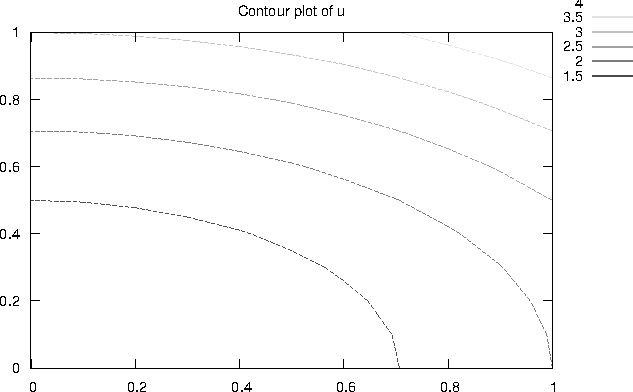
\includegraphics[width=5cm]{chapters/langtangen/pdf/Poisson2D_Dvc_contour1.pdf}}
    \subfloat[]{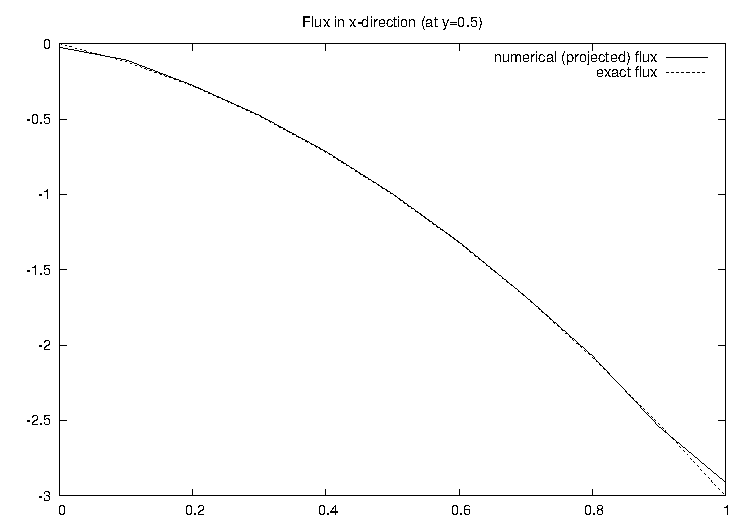
\includegraphics[width=5cm]{chapters/langtangen/pdf/Poisson2D_Dvc_flux_x.pdf}}
  \end{center}
  \caption{Examples on plots created by transforming the finite
    element field to a field on a uniform, structured 2D grid: (a)
    contour plot of the solution; (b) curve plot of the exact flux
    $-p\partial u/\partial x$ against the corresponding projected
    numerical flux.}
  \label{langtangen:poisson:2D:fig2}
\end{figure}

\begin{figure}
  \begin{center}
    \subfloat[]{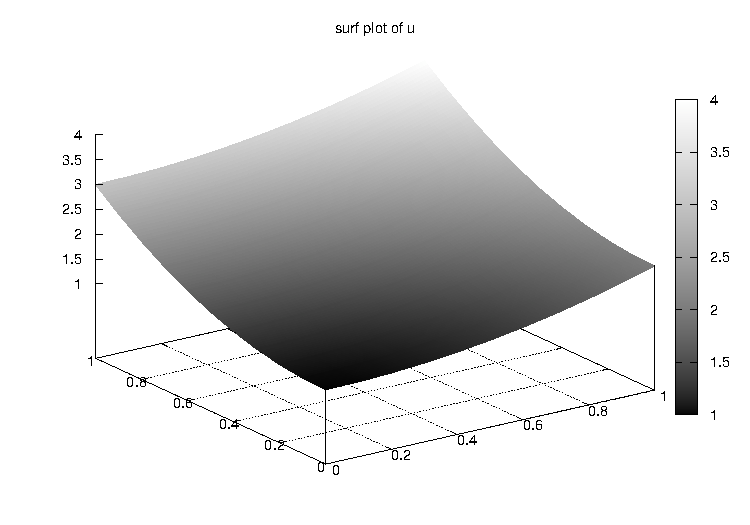
\includegraphics[width=5cm]{chapters/langtangen/pdf/Poisson2D_Dvc_surf1.pdf}}
    \subfloat[]{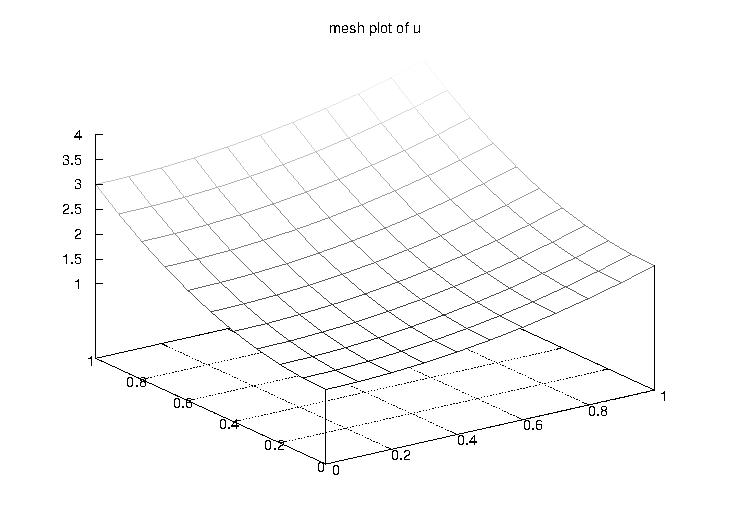
\includegraphics[width=5cm]{chapters/langtangen/pdf/Poisson2D_Dvc_mesh1.pdf}}
  \end{center}
  \caption{Examples on plots created by transforming the finite
    element field to a field on a uniform, structured 2D grid: (a) a
    surface plot of the solution; (b) lifted mesh plot of the
  solution.}
  \label{langtangen:poisson:2D:fig3}
\end{figure}

It should be easy with the information above to transform a finite element
field over a uniform rectangular or box-shaped mesh to the corresponding
\emp{BoxField} object and perform MATLAB-style
visualizations of the whole field or
the field over planes or along lines through the domain.
By the transformation to a regular grid we have some more flexibility
than what Viper offers. (It should be added that
comprehensive tools like
VisIt, MayaVi2, or ParaView also have the possibility for plotting fields
along lines and extracting planes in 3D geometries, though usually with
less degree of control compared to Gnuplot, MATLAB, and matplotlib.)

\subsection{Parameterizing the number of space dimensions}
\label{langtangen:poisson:nD}
\index{dimension-independent code}

\fenics{} makes it is easy to write a unified simulation code that can operate
in 1D, 2D, and 3D. We will conveniently make use of this feature in
forthcoming examples. The relevant technicalities are therefore explained
below.

Consider the simple problem
\begin{equation}
u''(x) = 2\hbox{ in }[0,1],\quad u(0)=0,\ u(1)=1,
\end{equation}
with exact solution $u(x)=x^2$. Our aim is to formulate and solve this
problem in a 2D and a 3D domain as well.
We may generalize the domain $[0,1]$ to a box of any size
in the $y$ and $z$ directions and pose homogeneous Neumann
conditions $\partial u/\partial n = 0$ at all additional boundaries
$y=\mbox{const}$ and $z=\mbox{const}$ to ensure that $u$ only varies with
$x$. For example, let us choose
a unit hypercube as domain: $\Omega = [0,1]^d$, where $d$ is the number
of space dimensions. The generalized $d$-dimensional Poisson problem
then reads
\begin{equation} \label{langtangen:poisson1:ddim}
  \begin{array}{rcll}
    \Delta u &=& 2 &\mbox{in } \Omega, \\
    u &=& 0 &\mbox{on } \Gamma_0,\\
    u &=& 1 &\mbox{on } \Gamma_1,\\
\frac{\partial u}{\partial n} &=& 0 &\mbox{on } \partial\Omega\backslash\left(
\Gamma_0\cup\Gamma_1\right),
  \end{array}
\end{equation}
where $\Gamma_0$ is the side of the hypercube where $x=0$, and
where $\Gamma_1$ is the side where $x=1$.

Implementing \eqref{langtangen:poisson1:ddim} for any $d$ is no more
complicated than solving a problem with a specific number of dimensions.
The only non-trivial part of the code is actually to define the mesh.
We use the command-line to provide user-input to the program. The first argument
can be the degree of the polynomial in the finite element basis functions.
Thereafter, we supply the
cell divisions in the various spatial directions. The number of
command-line arguments will then imply the number of space dimensions.
For example, writing \emp{3 10 3 4} on the command-line means that
we want to approximate $u$ by piecewise polynomials of degree 3,
and that the domain is a three-dimensional cube with $10\times 3\times 4$
divisions in the $x$, $y$, and $z$ directions, respectively.
Each of the $10\times 3\times 4 = 120$ boxes will
be divided into six tetrahedra.
The Python code can be quite compact:
\begin{python}
degree = int(sys.argv[1])
divisions = [int(arg) for arg in sys.argv[2:]]
d = len(divisions)
domain_type = [UnitInterval, UnitSquare, UnitCube]
mesh = domain_type[d-1](*divisions)
V = FunctionSpace(mesh, "Lagrange", degree)
\end{python}
First note that although \emp{sys.argv[2:]} holds the divisions of
the mesh, all elements of the list \emp{sys.argv[2:]} are string objects,
so we need to explicitly convert each element to an integer.
The construction \emp{domain\_type[d-1]} will pick the right name of the
object used to define the domain and generate the mesh.
Moreover, the argument \emp{*divisions}
sends each component of the list \emp{divisions} as a separate
argument. For example, in a 2D problem where \emp{divisions} has
two elements, the statement
\begin{python}
mesh = domain_type[d-1](*divisions)
\end{python}
is equivalent to
\begin{python}
mesh = UnitSquare(divisions[0], divisions[1])
\end{python}

The next part of the program is to set up the boundary conditions.
Since the Neumann conditions have $\partial u/\partial n=0$ we can
omit the boundary integral from the weak form. We then only
need to take care of Dirichlet conditions at two sides:
\begin{python}
tol = 1E-14   # tolerance for coordinate comparisons
def Dirichlet_boundary0(x, on_boundary):
    return on_boundary and abs(x[0]) < tol

def Dirichlet_boundary1(x, on_boundary):
    return on_boundary and abs(x[0] - 1) < tol

bc0 = DirichletBC(V, Constant(0), Dirichlet_boundary0)
bc1 = DirichletBC(V, Constant(1), Dirichlet_boundary1)
bc = [bc0, bc1]
\end{python}
Note that this code is independent of the number of space dimensions.
So are the statements defining and solving
the variational problem:
\begin{python}
u = TrialFunction(V)
v = TestFunction(V)
f = Constant(-2)
a = inner(grad(u), grad(v))*dx
L = f*v*dx

problem = VariationalProblem(a, L, bc)
u = problem.solve()
\end{python}
The complete code is found in \emp{Poisson123D\_DN1.py}.

Observe that if we actually want to test variations in one selected
space direction, parameterized by \emp{e},
we only need to replace \emp{x[0]} in the
code by \emp{x[e]}. The parameter
\emp{e} could be given as the second
command-line argument.  This extension appears in the file
\emp{Poisson123D\_DN2.py}.  You can run a 3D
problem with this code where $u$ varies in, e.g., $z$ direction and is
approximated by, e.g., a 5-th degree polynomial.  For any legal input
the numerical solution coincides with the exact solution at the nodes
(because the exact solution is a second-degree polynomial).

\section{Nonlinear problems}
\label{langtangen:poisson:nonlinear}
\label{nonlinear PDEs}

Now we shall address how to solve nonlinear PDEs in \fenics. Our
sample PDE for implementation is taken as a nonlinear Poisson
equation:
\begin{equation}
-\nabla\cdot\left( q(u)\nabla u\right) = f.
\end{equation}
The coefficient $q(u)$ makes the equation nonlinear (unless $q(u)$
is a constant).

To be able to easily verify our implementation, we choose the domain,
$q(u)$, $f$, and the boundary conditions such that we have a simple,
exact solution $u$. Let $\Omega$ be the unit hypercube $[0, 1]^d$ in
$d$ dimensions, $q(u)=(1+u)^m$, $f=0$, $u=0$ for $x_0=0$, $u=1$ for
$x_0=1$, and $\partial u/\partial n=0$ at all other boundaries $x_i=0$
and $x_i=1$, $i=1,\ldots,d-1$. The coordinates are now represented by
the symbols $x_0,\ldots,x_{d-1}$. The exact solution is then
\begin{equation}
u(x_0,\ldots,x_d) = \left((2^{m+1}-1)x_0 + 1\right)^{1/(m+1)} - 1.
\end{equation}

The variational formulation of our model problem reads:
find $u \in V$ such that
\begin{equation} \label{langtangen:poisson:nonlinear1}
  F(u; v) = 0 \quad \foralls v \in \hat{V},
\end{equation}
where
\begin{equation}
\label{langtangen:poisson:nonlinear2}
F(u; v) = \int_\Omega q(u)\nabla u\cdot \nabla v\dx,
\end{equation}
and
\begin{equation}
  \begin{split}
    \hat{V} &= \{v \in H^1(\Omega) : v = 0 \mbox{ on } x_0=0\mbox{ and }x_0=1\}, \\
     V      &= \{v \in H^1(\Omega) : v = 0 \mbox{ on } x_0=0\mbox{ and } v = 1\mbox{ on }x_0=1\}. \\
  \end{split}
\end{equation}
The discrete problem arises as usual by restricting $V$ and $\hat V$
to a pair of discrete spaces. As usual, we omit any subscript on
discrete spaces and simply say $V$ and $\hat V$ are chosen finite
dimensional according to some mesh and element type.  The nonlinear
problem then reads: find $u\in V$ such that
\begin{equation}
  F(u; v) = 0 \quad \foralls v \in \hat{V},
\label{langtangen:poisson:nonlinear:d}
\end{equation}
with $u = \sum_{j=1}^N U_j \phi_j$. Since $F$ is a nonlinear function
of $u$, \eqref{langtangen:poisson:nonlinear:d} gives rise to a system
of nonlinear algebraic equations.  From now on the interest is only in
the discrete problem, and as mentioned in
Section~\ref{langtangen:poisson1:varform}, we simply write $u$ instead
of $u_h$ to get a closer resemblance in notation between the mathematics and the
Python code. When the exact solution needs to be distinguished, we
denote it by $u_e$.

\fenics{} can be used in alternative ways for solving a nonlinear PDE
problem. We shall in the following subsections go through four
solution strategies:
1) a simple Picard-type iteration,
2) a Newton method at the algebraic level,
3) a Newton method at the PDE level, and
4) an automatic approach where \fenics{} attacks the nonlinear variational
problem directly. The ``black box'' strategy 4) is definitely the
simplest one from a
programmer's point of view, but the others give more control of the
solution process for nonlinear equations (which also has some
pedagogical advantages).

\subsection{Picard iteration}
\label{langtangen:nonlinear:Picard}
\index{Picard iteration}
\index{successive substitutions}

Picard iteration is an easy way of handling nonlinear PDEs: we simply
use a known, previous solution in the nonlinear terms so that these
terms become linear in the unknown $u$. The strategy is also known as
the method of successive substitutions.
For our particular problem,
we use a known, previous solution in the coefficient $q(u)$.
More precisely, given a solution $u^k$ from iteration $k$, we seek a
new (hopefully improved) solution $u^{k+1}$ in iteration $k+1$ such
that $u^{k+1}$ solves the \emph{linear problem}
\begin{equation}
\label{langtangen:poisson:nonlinear:picard1}
\nabla\cdot \left(q(u^k)\nabla u^{k+1}\right) = 0,\quad k=0,1,\ldots
\end{equation}
The iterations require an initial guess $u^0$.
The hope is that $u^{k} \rightarrow u$ as $k\rightarrow\infty$, and that
$u^{k+1}$ is sufficiently close to the exact
solution $u$ of the discrete problem after just a few iterations.

We can easily formulate a variational problem for $u^{k+1}$ from
Equation~\eqref{langtangen:poisson:nonlinear:picard1}.
Equivalently, we can approximate $q(u)$ by $q(u^k)$ in
\eqref{langtangen:poisson:nonlinear2}
to obtain the same linear variational problem.
In both cases, the problem consists of seeking
$u^{k+1} \in V$ such that
\begin{equation} \label{langtangen:poisson:nonlinear:picard2}
  \tilde F(u^{k+1}; v) = 0 \quad \foralls v \in \hat{V},\quad k=0,1,\ldots,
\end{equation}
with
\begin{equation}
\label{langtangen:poisson:nonlinear:picard3}
\tilde F(u^{k+1}; v) = \int_\Omega q(u^k)\nabla u^{k+1}\cdot \nabla v\dx
.
\end{equation}
Since this is a linear problem in the unknown $u^{k+1}$, we can equivalently
use the formulation
\begin{equation}
a(u^{k+1},v) = L(v),
\end{equation}
with
\begin{align}
a(u,v) &= \int_\Omega q(u^k)\nabla u\cdot \nabla v\dx,
\\
L(v) &= 0.
\end{align}

The iterations can be stopped when $\epsilon\equiv ||u^{k+1}-u^k||
< \mathrm{tol}$, where $\mathrm{tol}$ is small, say $10^{-5}$, or
when the number of iterations exceed some critical limit. The latter
case will pick up divergence of the method or unacceptable slow
convergence.

In the solution algorithm we only need to store $u^k$ and $u^{k+1}$,
called \emp{uk} and \emp{u} in the code below.
The algorithm can then be expressed as follows:
\begin{python}
def q(u):
    return (1+u)**m

# Define variational problem
u = TrialFunction(V)
v = TestFunction(V)
uk = interpolate(Expression("0.0"), V)  # previous (known) u
a = inner(q(uk)*grad(u), grad(v))*dx
f = Constant(0.0)
L = f*v*dx

# Picard iterations
u = Function(V)     # new unknown function
eps = 1.0           # error measure ||u-uk||
tol = 1.0E-5        # tolerance
iter = 0            # iteration counter
maxiter = 25        # max no of iterations allowed
while eps > tol and iter < maxiter:
    iter += 1
    problem = VariationalProblem(a, L, bc)
    u = problem.solve()
    diff = u.vector().array() - uk.vector().array()
    eps = numpy.linalg.norm(diff, ord=numpy.Inf)
    print "Norm, iter=%d: %g" % (iter, eps)
    uk.assign(u)    # update for next iteration
\end{python}
We need to define the previous solution in the iterations,
\emp{uk}, as a finite element function so
that \emp{uk} can be updated with
\emp{u} at the end of the loop. We may
create the initial \emp{Function}
\emp{uk} by interpolating an
\emp{Expression} or a
\emp{Constant} to the same vector space as
\emp{u} lives in
(\emp{V}).

In the code above we demonstrate how to use
\emp{numpy} functionality to compute the
norm of the difference between the two most recent solutions. Here we
apply the maximum norm ($\ell_\infty$ norm) on the difference of the
solution vectors (\emp{ord=1} and
\emp{ord=2} give the $\ell_1$ and $\ell_2$
vector norms -- other norms are possible for
\emp{numpy} arrays, see
\emp{pydoc numpy.linalg.norm}).

The file \emp{nlPoisson\_Picard.py} contains
the complete code for this problem. The implementation is $d$
dimensional, with mesh construction and setting of Dirichlet
conditions as explained in Section~\ref{langtangen:poisson:nD}.  For a
$33\times 33$ grid with $m=2$ we need 9 iterations for convergence
when the tolerance is $10^{-5}$.

\subsection{A Newton method at the algebraic level}
\label{langtangen:nonlinear:Newton:algebraic}
\label{Newton's method algebraic}

After having discretized our nonlinear PDE problem, we may
use Newton's method to solve the system of nonlinear algebraic equations.
From the continuous variational problem \eqref{langtangen:poisson:nonlinear1},
the discrete version \eqref{langtangen:poisson:nonlinear:d} results in a
system of equations for the unknown parameters $U_1,\ldots, U_N$
(by inserting $u = \sum_{j=1}^N U_j \phi_j$
and $v=\hat\phi_i$ in \eqref{langtangen:poisson:nonlinear:d}):
\begin{equation}
\label{langtangen:nonlinear:Newton:F1}
F_i(U_1,\ldots,U_N) \equiv
\sum_{j=1}^N
\int_\Omega \left( q\left(\sum_{\ell=1}^NU_\ell\phi_\ell\right)
\nabla \phi_j U_j\right)\cdot \nabla \hat\phi_i\dx = 0,\quad i=1,\ldots,N.
\end{equation}
Newton's method for the system $F_i(U_1,\ldots,U_j)=0$, $i=1,\ldots,N$
can be formulated as
\begin{align}
\sum_{j=1}^N
\frac{\partial}{\partial U_j} F_i(U_1^k,\ldots,U_N^k)\delta U_j
  &= -F_i(U_1^k,\ldots,U_N^k),\quad i=1,\ldots,N,
\\
U_j^{k+1} &= U_j^k + \omega\delta U_j,\quad j=1,\ldots,N,
\end{align}
where $\omega\in [0,1]$ is a relaxation parameter, and $k$ is an
iteration index. An initial guess $u^0$ must be provided to start the
algorithm.  The original Newton method has $\omega=1$, but in problems
where it is difficult to obtain convergence, so-called
\emph{under-relaxation}\index{under-relaxation} with $\omega < 1$ may
help.

We need, in a program, to compute the Jacobian matrix $\partial
F_i/\partial U_j$ and the right-hand side vector $-F_i$.  Our present
problem has $F_i$ given by \eqref{langtangen:nonlinear:Newton:F1}.
The derivative $\partial F_i/\partial U_j$ becomes
\begin{equation}
\int\limits_\Omega \left\lbrack
 q'(\sum_{\ell=1}^NU_\ell^k\phi_\ell)\phi_j
\nabla (\sum_{j=1}^NU_j^k\phi_j)\cdot \nabla \hat\phi_i
+
q\left(\sum_{\ell=1}^NU_\ell^k\phi_\ell\right)
\nabla \phi_j \cdot \nabla \hat\phi_i
\right\rbrack
\dx.
\label{langtangen:poisson:nonlinear:dFdU}
\end{equation}
The following results were used to obtain \eqref{langtangen:poisson:nonlinear:dFdU}:
\begin{equation}
\frac{\partial u}{\partial U_j} = \frac{\partial}{\partial U_j}
\sum_{j=1}^NU_j\phi_j = \phi_j,\quad \frac{\partial}{\partial U_j}\nabla u
      = \nabla\phi_j,\quad \frac{\partial}{\partial U_j}q(u) = q'(u)\phi_j.
\end{equation}
We can reformulate the Jacobian matrix
in \eqref{langtangen:poisson:nonlinear:dFdU} by introducing the short
notation $u^k = \sum_{j=1}^NU_j^k\phi_j$:
\begin{equation}
\frac{\partial F_i}{\partial U_j} =
\int_\Omega \left\lbrack
q'(u^k)\phi_j
\nabla u^k \cdot \nabla \hat\phi_i
+
q(u^k)
\nabla \phi_j \cdot \nabla \hat\phi_i
\right\rbrack
\dx.
\end{equation}
In order to make \fenics{} compute this matrix, we need to formulate a
corresponding variational problem. Looking at the
linear system of equations in Newton's method,
\[ \sum_{j=1}^N \frac{\partial F_i}{\partial U_j}\delta U_j = -F_i,\quad
i=1,\ldots,N,\]
we can introduce $v$ as a general test function replacing $\hat\phi_i$,
and we can identify the unknown
$\delta u = \sum_{j=1}^N\delta U_j\phi_j$. From the linear system
we can now go ``backwards'' to construct the corresponding
discrete weak form
\begin{equation}
\label{langtangen:nonlinear:Newton:aLF}
\int_\Omega \left\lbrack
q'(u^k)\delta u
\nabla u^k \cdot \nabla v
+
q(u^k)
\nabla \delta u\cdot \nabla v
\right\rbrack
\dx = - \int_\Omega q(u^k)
\nabla u^k\cdot \nabla v \dx.
\end{equation}
Equation \eqref{langtangen:nonlinear:Newton:aLF} fits the standard form
$a(\delta u,v)=L(v)$ with
\begin{align}
a(\delta u,v) &= \int_\Omega \left\lbrack q'(u^k)\delta u \nabla u^k \cdot \nabla v
  + q(u^k) \nabla \delta u \cdot \nabla v \right\rbrack \dx
\\
L(v) &= - \int_\Omega q(u^k) \nabla u^k\cdot \nabla v \dx.
\end{align}
Note the important feature in Newton's method that the previous solution
$u^k$ replaces $u$ in the formulas when computing the matrix $\partial
F_i/\partial U_j$ and vector $F_i$ for the linear system in each Newton
iteration.

We now turn to the implementation.  To obtain a good
initial guess $u^0$, we can solve a simplified, linear
problem, typically with $q(u)=1$, which yields the standard
Laplace equation $\Delta u^0 =0$. The recipe for solving this
problem appears in Sections~\ref{langtangen:poisson1:varform},
\ref{langtangen:poisson1:impl}, and \ref{langtangen:poisson1:DN}.
The code for computing $u^0$ becomes as follows:
\begin{python}
tol = 1E-14
def left_boundary(x, on_boundary):
    return on_boundary and abs(x[0]) < tol

def right_boundary(x, on_boundary):
    return on_boundary and abs(x[0]-1) < tol

Gamma_0 = DirichletBC(V, Constant(0.0), left_boundary)
Gamma_1 = DirichletBC(V, Constant(1.0), right_boundary)
bc = [Gamma_0, Gamma_1]

# Define variational problem for initial guess (q(u)=1, m=0)
u = TrialFunction(V)
v = TestFunction(V)
a = inner(grad(u), grad(v))*dx
f = Constant(0.0)
L = f*v*dx
A, b = assemble_system(a, L, bc_u)
uk = Function(V)
solve(A, uk.vector(), b)
\end{python}
Here, \emp{uk} denotes the solution function for the previous
iteration, so that the solution
after each Newton iteration is \emp{u = uk + omega*du}.
Initially, \emp{uk} is the initial guess we call $u^0$ in the mathematics.

The Dirichlet boundary conditions for the problem to be solved in each Newton
iteration are somewhat different than the conditions for $u$.
Assuming that $u^k$ fulfills the
Dirichlet conditions for $u$, $\delta u$ must be zero at the boundaries
where the Dirichlet conditions apply, in order for $u^{k+1}=u^k + \omega\delta u$ to fulfill
the right Dirichlet values. We therefore define an additional list of
Dirichlet boundary conditions objects for $\delta u$:
\begin{python}
Gamma_0_du = DirichletBC(V, Constant(0), LeftBoundary())
Gamma_1_du = DirichletBC(V, Constant(0), RightBoundary())
bc_du = [Gamma_0_du, Gamma_1_du]
\end{python}
The nonlinear coefficient and its derivative must be defined
before coding the weak form of the Newton system:
\begin{python}
def q(u):
    return (1+u)**m

def Dq(u):
    return m*(1+u)**(m-1)

du = TrialFunction(V) # u = uk + omega*du
a = inner(q(uk)*grad(du), grad(v))*dx + \
    inner(Dq(uk)*du*grad(uk), grad(v))*dx
L = -inner(q(uk)*grad(uk), grad(v))*dx
\end{python}

The Newton iteration loop is very similar to the Picard iteration loop
in Section~\ref{langtangen:nonlinear:Picard}:
\begin{python}
du = Function(V)
u  = Function(V)  # u = uk + omega*du
omega = 1.0       # relaxation parameter
eps = 1.0
tol = 1.0E-5
iter = 0
maxiter = 25
while eps > tol and iter < maxiter:
    iter += 1
    A, b = assemble_system(a, L, bc_du)
    solve(A, du.vector(), b)
    eps = numpy.linalg.norm(du.vector().array(), ord=numpy.Inf)
    print "Norm:", eps
    u.vector()[:] = uk.vector() + omega*du.vector()
    uk.assign(u)
\end{python}
There are other ways of implementing the
update of the solution as well:
\begin{python}
u.assign(uk)  # u = uk
u.vector().axpy(omega, du.vector())

# or
u.vector()[:] += omega*du.vector()
\end{python}
The \emp{axpy(a, y)} operation adds a scalar \emp{a} times a
\emp{Vector} \emp{y} to a \emp{Vector} object.  It is usually a fast
operation calling up an optimized BLAS routine for the calculation.

Mesh construction for a $d$-dimensional problem with arbitrary degree
of the Lagrange elements can be done as explained in
Section~\ref{langtangen:poisson:nD}.  The complete program appears in
the file \emp{nlPoisson\_algNewton.py}.

\subsection{A Newton method at the PDE level}
\label{langtangen:nonlinear:Newton:pdelevel}
\label{Newton's method}

Although Newton's method in PDE problems is normally formulated at the
linear algebra level; that is, as a solution method for systems of nonlinear
algebraic equations, we can also formulate the method at the PDE level.
This approach yields a linearization of the PDEs before they are discretized.
\fenics{} users will probably find this technique simpler to apply than
the more standard method of Section~\ref{langtangen:nonlinear:Newton:algebraic}.

Given an approximation to the solution field, $u^k$, we seek a
perturbation $\delta u$ so that
\begin{equation}
u^{k+1} = u^k + \delta u
\end{equation}
fulfills the nonlinear PDE.
However, the problem for $\delta u$ is still nonlinear and nothing is
gained. The idea is therefore to assume that $\delta u$ is sufficiently
small so that we can linearize the problem with respect to $\delta u$.
Inserting $u^{k+1}$ in the PDE,
linearizing the $q$ term as
\begin{equation}
q(u^{k+1}) = q(u^k) + q'(u^k)\delta u + {\cal O}((\delta u)^2)
\approx q(u^k) + q'(u^k)\delta u,
\end{equation}
and dropping other nonlinear terms in $\delta u$,
we get
\[
\nabla\cdot\left( q(u^k)\nabla u^k\right) +
\nabla\cdot\left( q(u^k)\nabla\delta u\right) +
\nabla\cdot\left( q'(u^k)\delta u\nabla u^k\right) = 0.
\]
We may collect the terms with the unknown $\delta u$ on the left-hand side,
\begin{equation}
\nabla\cdot\left( q(u^k)\nabla\delta u\right) +
\nabla\cdot\left( q'(u^k)\delta u\nabla u^k\right) =
-\nabla\cdot\left( q(u^k)\nabla u^k\right),
\end{equation}
The weak form of this PDE is derived by multiplying by a test function $v$
and integrating over $\Omega$, integrating the second-order derivatives
by parts:
\begin{equation}
\int_\Omega \left(
q(u^k)\nabla\delta u\cdot \nabla v
+ q'(u^k)\delta u\nabla u^k\cdot \nabla v\right)\dx
= -\int_\Omega q(u^k)\nabla u^k\cdot \nabla v\dx.
\end{equation}
The variational problem reads: find $\delta u\in V$ such that
$a(\delta u,v) = L(v)$ for all $v\in \hat V$, where
\begin{align}
a(\delta u,v) &= \int_\Omega \left( q(u^k)\nabla\delta u\cdot \nabla v
+ q'(u^k)\delta u\nabla u^k\cdot \nabla v\right)\dx,
\label{langtangen:nonlinear:poisson:pdelevel:eqa}
\\
L(v) &= - \int_\Omega q(u^k)\nabla u^k\cdot \nabla v\dx.
\label{langtangen:nonlinear:poisson:pdelevel:eqL}
\end{align}
The function spaces $V$ and $\hat V$, being continuous
or discrete, are as in the linear Poisson problem from
Section~\ref{langtangen:poisson1:varform}.

We must provide some initial guess, e.g., the solution of the
PDE with $q(u)=1$. The corresponding weak form $a_0(u^0,v)=L_0(v)$
has
\begin{equation}
a_0(u,v)=\int_\Omega\nabla u\cdot \nabla v\dx,\quad
L(v)=0.
\end{equation}
Thereafter, we enter a loop and solve $a(\delta u,v)=L(v)$ for $\delta
u$ and compute a new approximation $u^{k+1} = u^k + \delta u$. Note
that $\delta u$ is a correction, so if $u^0$ satisfies the prescribed
Dirichlet conditions on some part $\Gamma_D$ of the boundary, we must
demand $\delta u=0$ on $\Gamma_D$.

Looking at \eqref{langtangen:nonlinear:poisson:pdelevel:eqa} and
\eqref{langtangen:nonlinear:poisson:pdelevel:eqL}, we see that the
variational form is the same as for the Newton method at the algebraic
level in Section~\ref{langtangen:nonlinear:Newton:algebraic}. Since
Newton's method at the algebraic level required some ``backward''
construction of the underlying weak forms, \fenics{} users may prefer
Newton's method at the PDE level, which is more straightforward.  There is
seemingly no need for differentiations to derive a Jacobian matrix, but
a mathematically equivalent derivation is done when nonlinear terms are
linearized using the first two Taylor series terms and when products in
the perturbation $\delta u$ are neglected.

The implementation is identical to the one in
Section~\ref{langtangen:nonlinear:Newton:algebraic} and is found in
the file \emp{nlPoisson\_pdeNewton.py} (for the fun of it we use
a \emp{VariationalProblem} object instead of assembling a matrix and
vector and calling \emp{solve}). The reader is encouraged to go
through this code to be convinced that the present method actually
ends up with the same program as needed for the Newton method at
the linear algebra level in Section~\ref{langtangen:nonlinear:Newton:algebraic}.

\subsection{Solving the nonlinear variational problem directly}
\label{langtangen:nonlinear:Newton:auto}

DOLFIN has a built-in Newton solver and is able to automate the
computation of nonlinear, stationary boundary-value problems.
The automation is demonstrated next. A nonlinear variational
problem \eqref{langtangen:poisson:nonlinear1} can be solved by
\begin{python}
VariationalProblem(J, F, bc)
\end{python}
where \emp{F} corresponds to the nonlinear form $F(u;v)$ and
\emp{J} is a form for the derivative of \emp{F}.

The \emp{F} form corresponding to \eqref{langtangen:poisson:nonlinear2}
is straightforwardly defined (assuming \emp{q(u)} is
coded as a Python function):
\begin{python}
v = TestFunction(V)
u = Function(V)  # the unknown
F = inner(q(u)*grad(u), grad(v))*dx
\end{python}
Note here that \emp{u} is a \emp{Function}, not a \emp{TrialFunction}.
We could, alternatively, define $F(u;v)$ directly in terms of
a trial function for $u$ and a test function for $v$, and then
created the proper \emp{F} by
\begin{python}
u = TrialFunction(V)
v = TestFunction(V)
Fuv = inner(q(u)*grad(u), grad(v))*dx
u = Function(V)  # previous guess
F = action(Fuv, u)
\end{python}
The latter statement is equivalent to $F(u=u_0; v)$, where $u_0$ is
an existing finite element function representing the most recently
computed approximation to the solution.

The derivative $J$ (\emp{J}) of $F$ (\emp{F}) is formally the
Gateaux derivative $DF(u^k; \delta u, v)$
of $F(u;v)$ at $u=u^k$ in the direction of $\delta u$.
Technically, this Gateaux derivative is derived by computing
\index{Gateaux derivative}
\begin{equation}
  \lim_{\epsilon\rightarrow 0} \frac{d}{d\epsilon} F_i(u^k + \epsilon\delta u; v)
\label{langtangen:poisson:nonlinear:Gateaux1}
\end{equation}
The $\delta u$ is now the trial function and $u^k$ is as usual the previous
approximation to the solution $u$.
We start with
\begin{equation}
\frac{d}{d\epsilon}\int_\Omega \nabla v\cdot\left( q(u^k + \epsilon\delta u)
\nabla (u^k + \epsilon\delta u)\right)\dx
\end{equation}
and obtain
\begin{equation}
\int_\Omega \nabla v\cdot\left\lbrack
q'(u^k + \epsilon\delta u)\delta u
\nabla (u^k + \epsilon\delta u)
+
q(u^k + \epsilon\delta u)
\nabla \delta u
\right\rbrack\dx,
\end{equation}
which leads to
\begin{equation}
\int_\Omega \nabla v\cdot\left\lbrack
q'(u^k)\delta u
\nabla (u^k)
+
q(u^k)
\nabla \delta u
\right\rbrack\dx,
\end{equation}
as $\epsilon\rightarrow 0$.  This last expression is the Gateaux
derivative of $F$. We may use $J$ or $a(\delta u, v)$ for this derivative,
the latter having the advantage that we easily recognize the expression
as a bilinear form. However, in the forthcoming code examples \emp{J}
is used as variable name for the Jacobian.  The specification of \emp{J}
goes as follows:
\begin{python}
du = TrialFunction(V)
J = inner(q(u)*grad(du), grad(v))*dx + \
    inner(Dq(u)*du*grad(u), grad(v))*dx
\end{python}
where \emp{u} is a \emp{Function} representing the most recent solution.

The UFL language that we use to specify weak forms supports differentiation
of forms. This means that when \emp{F} is given as above, we can simply
compute the Gateaux derivative by\index{derivative}
\begin{python}
J = derivative(F, u, du)
\end{python}
The differentiation is done symbolically so no numerical approximation
formulas are involved. The \emp{derivative} function is obviously
very convenient in problems where differentiating \emp{F} by hand
implies lengthy calculations.

The solution of the nonlinear problem is now a question of two statements:
\index{nonlinear variational problems}
\begin{python}
problem = VariationalProblem(J, F, bc)
u = problem.solve(u)
\end{python}
The \emp{u} we feed to \emp{problem.solve} is filled with the solution
and returned, implying that the \emp{u} on the left-hand side actually
refers to the same \emp{u} as provided on the right-hand side\footnote{Python
has a convention that all input data to a function or class method are
represented as arguments, while all output data are returned to the calling
code. Data used as both input and output, as in this case, will then be
arguments and returned. It is not necessary to have a variable on the
left-hand side, as the function object is modified correctly anyway,
but it is convention that we follow here.}.
The file \emp{nlPoisson\_vp1.py} contains the complete code, where
\emp{J} is calculated manually, while \emp{nlPoisson\_vp2.py} is
a counterpart where \emp{J} is computed by \emp{derivative(F, u, du)}.
The latter file represents clearly the most automated way of solving
the present nonlinear problem in \fenics.

\section{Time-dependent problems}
\label{langtangen:timedep}

The examples in Section~\ref{langtangen:fundamentals} illustrate that
solving linear, stationary PDE problems with the aid of \fenics{} is
easy and requires little programming.  That is, \fenics{} automates
the spatial discretization by the finite element method.  The solution
of nonlinear problems, as we showed in
Section~\ref{langtangen:poisson:nonlinear}, can also be automated
(see~Section~\ref{langtangen:nonlinear:Newton:auto}), but many
scientists will prefer to code the solution strategy of the nonlinear
problem themselves and experiment with various combinations of
strategies in difficult problems. Time-dependent problems are somewhat
similar in this respect: we have to add a time discretization scheme,
which is often quite simple, making it natural to explicitly code the
details of the scheme so that the programmer has full control.  We
shall explain how easily this is accomplished through examples.

\subsection{A diffusion problem and its discretization}
\label{langtangen:timedep:diffusion1}
\index{time-dependent PDEs}

Our time-dependent
model problem for teaching purposes is naturally the simplest
extension of the Poisson problem into the time domain; that is,
the diffusion problem
\begin{align}
\frac{\partial u}{\partial t} &= \Delta u + f \mbox{ in } \Omega, \hbox{ for } t>0,
\label{langtangen:diffusion:pde1}
\\
    u &= u_0 \mbox{ on } \partial \Omega,\hbox{ for } t>0,
\label{langtangen:diffusion:pde1:bc}
\\
    u &= I   \mbox{ at } t=0.
\label{langtangen:diffusion:pde1:ic}
\end{align}
Here, $u$ varies with space and time, e.g., $u=u(x,y,t)$ if the spatial
domain $\Omega$ is two-dimensional. The source function $f$ and the
boundary values $u_0$ may also vary with space and time.  The initial
condition $I$ is a function of space only.

A straightforward approach to solving time-dependent PDEs by the finite
element method is to first discretize the time derivative by a finite
difference approximation, which yields a recursive set of stationary
problems, and then turn each stationary problem into a variational
formulation.

Let superscript $k$ denote a quantity at time $t_k$, where $k$ is an
integer counting time levels. For example, $u^k$ means $u$ at time
level $k$.  A finite difference discretization in time first consists
in sampling the PDE at some time level, say $k$:
\begin{equation}
  \frac{\partial}{\partial t}u^k = \Delta u^k + f^k.
\label{langtangen:diffusion:pde1:tk}
\end{equation}
The time-derivative can be approximated by a finite difference.
\index{finite difference time discretization}
For simplicity and stability reasons we choose a
simple backward difference:
\begin{equation}
  \frac{\partial}{\partial t} u^k\approx \frac{u^k - u^{k-1}}{\dt},
\label{langtangen:diffusion:BE}
\end{equation}
where ${\dt}$ is the time discretization parameter.
Inserting \eqref{langtangen:diffusion:BE} in \eqref{langtangen:diffusion:pde1:tk}
yields
\begin{equation}
  \frac{u^k - u^{k-1}}{\dt} = \Delta u^k + f^k.
\label{langtangen:diffusion:pde1:BE}
\end{equation}
This is our time-discrete version of the diffusion PDE \eqref{langtangen:diffusion:pde1}.
Reordering \eqref{langtangen:diffusion:pde1:BE} so that $u^k$ appears
on the left-hand side only, shows that \eqref{langtangen:diffusion:pde1:BE}
is a recursive set of
spatial (stationary) problems for $u^k$ (assuming $u^{k-1}$ is known from
computations at the previous time level):
\begin{align}
u^0 &= I,
\label{langtangen:diffusion:pde1:u0}
\\
u^k - {\dt}\Delta u^k &=  u^{k-1} + {\dt} f^k, \quad k=1,2,\ldots
\label{langtangen:diffusion:pde1:uk}
\end{align}
Given $I$, we can solve for $u^0$, $u^1$, $u^2$, and so on.

We use a finite element method to solve the
equations \eqref{langtangen:diffusion:pde1:u0} and
\eqref{langtangen:diffusion:pde1:uk}.  This requires turning the equations
into weak forms.  As usual, we multiply by a test function $v\in \hat V$
and integrate second-derivatives by parts. Introducing the symbol $u$
for $u^k$ (which is natural in the program too), the resulting weak form
can be conveniently written in the standard notation: $a_0(u,v)=L_0(v)$
for \eqref{langtangen:diffusion:pde1:u0} and $a(u,v)=L(v)$ for
\eqref{langtangen:diffusion:pde1:uk}, where
\begin{align}
a_0(u,v) &= \int_\Omega uv\dx,
\label{langtangen:diffusion:pde1:a0}
\\
L_0(v) &= \int_\Omega Iv\dx,
\label{langtangen:diffusion:pde1:L0}
\\
a(u,v) &= \int_\Omega\left( uv + {\dt} \nabla u\cdot \nabla v\right)\dx,
\label{langtangen:diffusion:pde1:a}
\\
L(v) &= \int_\Omega \left(u^{k-1} + {\dt}  f^k\right)v\dx.
\label{langtangen:diffusion:pde1:L}
\end{align}
The continuous variational problem is to find $u^0\in V$ such that
$a_0(u^0,v)=L_0(v)$ holds for all $v\in\hat V$, and then find $u^k\in V$
such that $a(u^k,v)=L(v)$ for all $v\in\hat V$, $k=1,2,\ldots$.

Approximate solutions in space are found by restricting the functional
spaces $V$ and $\hat V$ to finite-dimensional spaces, exactly as we have
done in the Poisson problems.  We shall use the symbol $u$ for the finite
element approximation at time $t_k$. In case we need to distinguish
this space-time discrete approximation from the exact solution of the
continuous diffusion problem, we use $u_e$ for the latter.  By $u^{k-1}$
we mean, from now on, the finite element approximation of the solution
at time $t_{k-1}$.

Note that the forms $a_0$ and $L_0$ are identical to the forms met in
Section~\ref{langtangen:poisson:gradu}, except that the test and trial
functions are now scalar fields and not vector fields.  Instead of
solving \eqref{langtangen:diffusion:pde1:u0} by a finite element method;
that is, projecting $I$ onto $V$ via the problem $a_0(u,v)=L_0(v)$, we
could simply interpolate $u^0$ from $I$. That is, if $u^0=\sum_{j=1}^N
U^0_j\phi_j$, we simply set $U_j=I(x_j,y_j)$, where $(x_j,y_j)$ are
the coordinates of node number $j$. We refer to these two strategies as
computing the initial condition by either projecting $I$ or interpolating
$I$.  Both operations are easy to compute through one statement, using
either the \emp{project} or \emp{interpolate} function.

\subsection{Implementation}
\label{langtangen:timedep:diffusion1:impl}

Our program needs to perform the time stepping explicitly, but can
rely on \fenics{} to easily compute $a_0$, $L_0$, $a$, and $L$, and
solve the linear systems for the unknowns.  We realize that $a$ does
not depend on time, which means that its associated matrix also will be
time independent. Therefore, it is wise to explicitly create matrices and
vectors as in Section~\ref{langtangen:poisson1:linalg}.  The matrix $A$
arising from $a$ can be computed prior to the time stepping, so that
we only need to compute the right-hand side $b$, corresponding to $L$,
in each pass in the time loop. Let us express the solution procedure
in algorithmic form, writing $u$ for $u^k$ and $u_{\rm prev}$ for the
previous solution $u^{k-1}$:
%%
\begin{quote}
\begin{tabbing}
\hspace*{0.5cm}\= \hspace{0.5cm} \= \hspace{0.5cm} \=
\hspace{0.5cm} \= \hspace{0.5cm} \= \kill
define Dirichlet boundary condition ($u_0$, Dirichlet boundary, etc.)\\
if $u_{\rm prev}$ is to be computed by projecting $I$:\\
\>define $a_0$ and $L_0$\\
\> assemble matrix $M$ from $a_0$ and vector $b$ from $L_0$\\
\> solve $MU=b$ and store $U$ in $u_{\rm prev}$\\
else:  (interpolation)\\
\> let $u_{\rm prev}$ interpolate $I$\\
define $a$ and $L$\\
assemble matrix $A$ from $a$\\
set some stopping time $T$\\
$t={\dt}$\\
while $t\leqslant T$\\
\> assemble vector $b$ from $L$\\
\> apply essential boundary conditions\\
\> solve $AU=b$ for $U$ and store in $u$\\
\> $t\leftarrow t + {\dt}$\\
\> $u_{\rm prev} \leftarrow u$ (be ready for next step)
\end{tabbing}
\end{quote}

Before starting the coding, we shall construct a problem where it is
easy to determine if the calculations are correct. The simple backward
time difference is exact for linear functions, so we decide to have
a linear variation in time. Combining a second-degree polynomial in space
with a linear term in time,
\begin{equation}
  u = 1 + x^2 + \alpha y^2 + \beta t,
\label{langtangen:diffusion:pde1:u0test}
\end{equation}
yields a function whose computed values at the nodes may be exact,
regardless of the size of the elements and ${\dt}$, as long as the mesh is
uniformly partitioned.  Inserting \eqref{langtangen:diffusion:pde1:u0test}
in the PDE problem \eqref{langtangen:diffusion:pde1}, it follows that
$u_0$ must be given as \eqref{langtangen:diffusion:pde1:u0test} and that
$f(x,y,t)=\beta - 2 - 2\alpha$ and $I(x,y)=1+x^2+\alpha y^2$.

A new programming issue is how to deal with functions that vary in
space \emph{and time}, such as the boundary condition $u_0$ given by
\eqref{langtangen:diffusion:pde1:u0test}.  Given a \emp{mesh} and an
associated function space \emp{V}, we can specify the $u_0$ function
as \index{\emp{Expression}}
\begin{python}
alpha = 3; beta = 1.2
u0 = Expression("1 + x[0]*x[0] + alpha*x[1]*x[1] + beta*t",
                {"alpha": alpha, "beta": beta})
u0.t = 0
\end{python}
This function expression has the components of \emp{x} as independent
variables, while \emp{alpha}, \emp{beta}, and \emp{t} are parameters.
The parameters can either be set through a dictionary at construction
time, as demonstrated for \emp{alpha} and \emp{beta}, or anytime through
attributes in the function object, as shown for the \emp{t} parameter.

The essential boundary conditions, along the whole boundary in this case,
are set in the usual way,
\begin{python}
def boundary(x, on_boundary):  # define the Dirichlet boundary
    return on_boundary

bc = DirichletBC(V, u0, boundary)
\end{python}

The initial condition can be computed by either projecting or
interpolating $I$. The $I(x,y)$ function is available in the program
through \emp{u0}, as long as \emp{u0.t} is zero.  We can then do
\begin{python}
u_prev = interpolate(u0, V)
# or
u_prev = project(u0, V)
\end{python}
Note that we could, as an equivalent alternative to using \emp{project},
define $a_0$ and $L_0$ as we did in Section~\ref{langtangen:poisson:gradu}
and form a \emp{VariationalProblem} object.  To actually recover
\eqref{langtangen:diffusion:pde1:u0test} to machine precision, it is
important not to compute the discrete initial condition by projecting
$I$, but by interpolating $I$ so that the nodal values are exact at $t=0$
(projection will imply approximative values at the nodes).

The definition of $a$ and $L$ goes as follows:
\begin{python}
dt = 0.3      # time step

u = TrialFunction(V)
v = TestFunction(V)
f = Constant(beta - 2 - 2*alpha)

a = u*v*dx + dt*inner(grad(u), grad(v))*dx
L = (u_prev + dt*f)*v*dx

A = assemble(a)   # assemble only once, before the time stepping
\end{python}

Finally, we perform the time stepping in a loop:
\begin{python}
u = Function(V)   # the unknown at a new time level
T = 2             # total simulation time
t = dt

while t <= T:
    b = assemble(L)
    u0.t = t
    bc.apply(A, b)
    solve(A, u.vector(), b)

    t += dt
    u_prev.assign(u)
\end{python}
Observe that \emp{u0.t} must be updated before \emp{bc} applies it to
enforce the Dirichlet conditions at the current time level.

The time loop above does not contain any examination of the numerical
solution, which we must include in order to verify the implementation.
As in many previous examples, we compute the difference between the
array of nodal values of \emp{u} and the array of the interpolated
exact solution.  The following code is to be included inside the loop,
after \emp{u} is found:
\begin{python}
    u_e = interpolate(u0, V)
    maxdiff = (u_e.vector().array() - u.vector().array()).max()
    print "Max error, t=%.2f: %-10.3f" % (t, maxdiff)
\end{python}

The right-hand side vector \emp{b} must obviously be recomputed at
each time level.  With the construction \emp{b = assemble(L)}, a new
vector for \emp{b} is allocated in memory in every pass of the time
loop.  It would be much more memory friendly to reuse the storage of
the \emp{b} we already have. This is easily accomplished
by\index{assemble}
\begin{python}
    b = assemble(L, tensor=b)
\end{python}
That is, we send in our previous \emp{b}, which is then filled with new
values and returned from \emp{assemble}. Now there will be only a single
memory allocation of the right-hand side vector. Before the time loop
we set \emp{b = None} such that \emp{b} is defined in the first call
to \emp{assemble}.

The complete program code for this time-dependent case is stored in the
file \emp{diffusion2D\_D1.py}.

\subsection{Avoiding assembly}
\label{langtangen:timedep:diffusion1:noassemble}
\index{assembly, increasing efficiency}

The purpose of this section is to present a technique for speeding up
\fenics{} simulators for time-dependent problems where it is possible
to perform all assembly operations prior to the time loop.  There are
two costly operations in the time loop: assembly of the right-hand side
$b$ and solution of the linear system via the \emp{solve} call. The
assembly process involves work proportional to the number of degrees of
freedom $N$, while the solve operation has a work estimate of ${\cal O}(
N^{\alpha})$, for some $\alpha\geqslant 1$. As $N\rightarrow\infty$, the
solve operation will dominate for $\alpha>1$, but for the values of $N$
typically used on smaller computers, the assembly step may still represent
a considerable part of the total work at each time level. Avoiding
repeated assembly can therefore contribute to a significant speed-up of
a finite element code in time-dependent problems.

To see how repeated assembly can be avoided, we look at the $L(v)$
form in \eqref{langtangen:diffusion:pde1:L}, which in general varies
with time through $u^{k-1}$, $f^k$, and possibly also with ${\dt}$
if the time step is adjusted during the simulation.  The technique
for avoiding repeated assembly consists in expanding the finite
element functions in sums over the basis functions $\phi_i$, as
explained in Section~\ref{langtangen:poisson1:linalg}, to identify
matrix-vector products that build up the complete system. We have
$u^{k-1}=\sum_{j=1}^NU^{k-1}_j\phi_j$, and we can expand $f^k$ as
$f^{k}=\sum_{j=1}^NF^{k}_j\phi_j$. Inserting these expressions in $L(v)$
and using $v=\hat\phi_i$ result in
\begin{equation}
\begin{split}
\int_\Omega \left(u^{k-1} + {\dt}f^k\right)v\dx
  &= \int_\Omega \left(\sum_{j=1}^N U^{k-1}_j\phi_j + {\dt}\sum_{j=1}^N F^{k}_j\phi_j\right)\hat\phi_i\dx,
\\
  &=\sum_{j=1}^N\left(\int_\Omega \hat\phi_i\phi_j\dx\right)U^{k-1}_j
 + {\dt}\sum_{j=1}^N\left(\int_\Omega \hat\phi_i\phi_j\dx\right)F^{k}_j.
\end{split}
\end{equation}
Introducing $M_{ij} = \int_\Omega \hat\phi_i\phi_j\dx$, we see that
the last expression can be written
\begin{equation}
  \sum_{j=1}^NM_{ij}U^{k-1}_j + {\dt} \sum_{j=1}^NM_{ij}F^{k}_j,
\end{equation}
which is nothing but two matrix-vector products,
\begin{equation}
   MU^{k-1} + {\dt} MF^k,
\end{equation}
if $M$ is the matrix with entries $M_{ij}$ and
\begin{equation}
  U^{k-1}=(U^{k-1}_1,\ldots,U^{k-1}_N)^{\top},
\end{equation}
and
\begin{equation}
 F^k=(F^{k}_1,\ldots,F^{k}_N)^{\top}.
\end{equation}

We have immediate access to $U^{k-1}$
in the program since that is the vector
in the \emp{u\_prev} function. The $F^k$ vector can easily be
computed by interpolating the prescribed $f$ function (at each time level if
$f$ varies with time). Given $M$, $U^{k-1}$, and $F^k$, the right-hand side
$b$ can be calculated as
\begin{equation}
 b = MU^{k-1} + {\dt} MF^k.
\end{equation}
That is, no assembly is necessary to compute $b$.

The coefficient matrix $A$ can also be split into two terms.
We insert $v=\hat\phi_i$ and $u^k = \sum_{j=1}^N U^k_j\phi_j$ in
the expression \eqref{langtangen:diffusion:pde1:a} to get
\begin{equation}
 \sum_{j=1}^N \left(\int_\Omega \hat\phi_i\phi_j\dx\right)U^k_j
+ {\dt} \sum_{j=1}^N \left(\int_\Omega \nabla\hat\phi_i\cdot\nabla\phi_j\dx\right)U^k_j,
\end{equation}
which can be written as a sum of matrix-vector products,
\begin{equation}
 MU^k + {\dt} KU^k = (M + {\dt} K)U^k,
\end{equation}
if we identify the matrix $M$ with entries $M_{ij}$ as above and
the matrix $K$ with entries
\begin{equation}
  K_{ij} = \int_\Omega \nabla\hat\phi_i\cdot\nabla\phi_j\dx.
\end{equation}
The matrix $M$ is often called the ``mass matrix'' while ``stiffness
matrix'' is a common nickname for $K$. The associated bilinear forms for
these matrices, as we need them for the assembly process in a \fenics{}
program, become
\begin{align}
  a_K(u,v) &= \int_\Omega\nabla u\cdot\nabla v\dx,
\label{langtangen:diffusion:pde1:aK}
\\
  a_M(u,v) &= \int_\Omega uv\dx.
\label{langtangen:diffusion:pde1:aM}
\end{align}

The linear system at each time level, written as $AU^k=b$, can now be
computed by first computing $M$ and $K$, and then forming $A=M+{\dt}
K$ at $t=0$, while $b$ is computed as $b=MU^{k-1} + {\dt}MF^k$ at each
time level.

The following modifications are needed in the \emp{diffusion2D\_D1.py}
program from the previous section in order to implement the new strategy
of avoiding assembly at each time level:
\begin{enumerate}
\item Define separate forms $a_M$ and $a_K$
\item Assemble $a_M$ to $M$ and $a_K$ to $K$
\item Compute $A=M+{\dt}\, K$
\item Define $f$ as an \emp{Expression}
\item Interpolate the formula for $f$ to a finite element function $F^k$
\item Compute $b=MU^{k-1} + {\dt}MF^k$
\end{enumerate}
The relevant code segments become
\begin{python}
# 1.
a_K = inner(grad(u), grad(v))*dx
a_M = u*v*dx

# 2. and 3.
M = assemble(a_M)
K = assemble(a_K)
A = M + dt*K

# 4.
f = Expression("beta - 2 - 2*alpha", {"beta": beta, "alpha": alpha})

# 5. and 6.
while t <= T:
    fk = interpolate(f, V)
    Fk = fk.vector()
    b = M*u_prev.vector() + dt*M*Fk
\end{python}
The complete program appears in the file \emp{diffusion2D\_D2.py}.

\subsection{A physical example}
\label{langtangen:timedep:diffusion2:sin}

With the basic programming techniques for time-dependent problems from
Sections~\ref{langtangen:timedep:diffusion1:noassemble}--\ref{langtangen:timedep:diffusion1:impl}
we are ready to attack more physically realistic examples.  The next
example concerns the question: How is the temperature in the ground
affected by day and night variations at the earth's surface?  We consider
some box-shaped domain $\Omega$ in $d$ dimensions with coordinates
$x_0,\ldots,x_{d-1}$ (the problem is meaningful in 1D, 2D, and 3D).
At the top of the domain, $x_{d-1}=0$, we have an oscillating temperature
\begin{equation}
  T_0(t) = T_R + T_A\sin (\omega t),
\end{equation}
where $T_R$ is some reference temperature, $T_A$ is the amplitude
of the temperature variations at the surface, and $\omega$ is the
frequency of the temperature oscillations.  At all other boundaries
we assume that the temperature does not change anymore when we
move away from the boundary; that is, the normal derivative is zero.
Initially, the temperature can be taken as $T_R$ everywhere.  The heat
conductivity properties of the soil in the ground may vary with space so
we introduce a variable coefficient $\kappa$ reflecting this property.
Figure~\ref{langtangen:timedep:diffusion2:sin:fig1} shows a sketch of the
problem, with a small region where the heat conductivity is much lower.
\begin{figure}
\centerline{
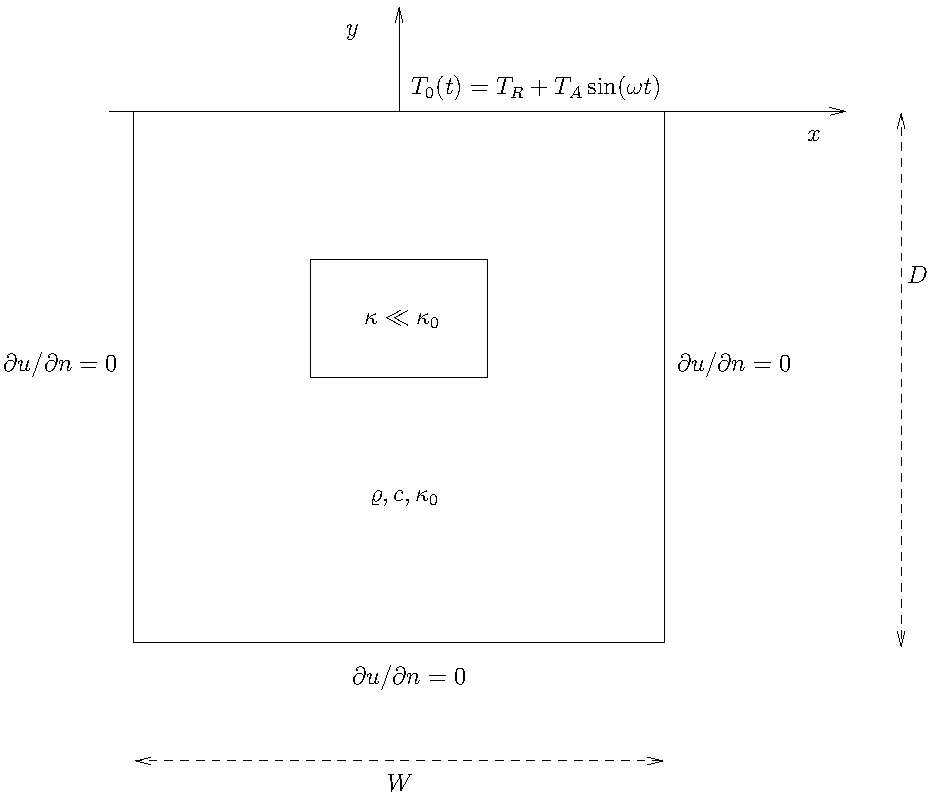
\includegraphics[width=0.8\linewidth]{chapters/langtangen/pdf/daynight.pdf}}
  \caption{Sketch of a (2D) problem involving heating and cooling of
  the ground due to an oscillating surface temperature}
\label{langtangen:timedep:diffusion2:sin:fig1}
\end{figure}

The initial-boundary value problem for this problem reads
\begin{align}
\varrho c \frac{\partial T}{\partial t}
    &= \nabla\cdot\left( \kappa\nabla T\right)\hbox{ in }\Omega\times (0,t_{\hbox{stop}}],
\\
T &= T_0(t)\hbox{ on }\Gamma_0,
\\
\frac{\partial T}{\partial n} &= 0\hbox{ on }\partial\Omega\backslash\Gamma_0,
\\
T &= T_R\hbox{ at }t =0.
\end{align}
Here, $\varrho$ is the density of the soil, $c$ is the heat capacity,
$\kappa$ is the thermal conductivity (heat conduction coefficient)
in the soil, and $\Gamma_0$ is the surface boundary $x_{d-1}=0$.

We use a $\theta$-scheme in time; that is, the evolution equation
$\partial P/\partial t=Q(t)$ is discretized as
\begin{equation}
   \frac{P^k - P^{k-1}}{\dt} = \theta Q^k + (1-\theta )Q^{k-1},
\end{equation}
where $\theta\in[0,1]$ is a weighting factor: $\theta =1$
corresponds to the backward difference scheme, $\theta =1/2$ to the
Crank--Nicolson scheme, and $\theta =0$ to a forward difference scheme.
The $\theta$-scheme applied to our PDE results in
\begin{equation}
\varrho c \frac{T^k-T^{k-1}}{\dt} =
\theta \nabla\cdot\left( \kappa\nabla T^k\right)
+ (1-\theta) \nabla\cdot\left( k\nabla T^{k-1}\right).
\end{equation}
Bringing this time-discrete PDE into weak form follows the technique
shown many times earlier in this tutorial. In the standard notation
$a(T,v)=L(v)$ the weak form has
\begin{align}
a(T,v) &= \int_\Omega
\left( \varrho c Tv + \theta{\dt} \kappa\nabla T\cdot \nabla v\right)\dx,
\\
L(v) &= \int_\Omega \left( \varrho c T^{k-1}v - (1-\theta){\dt}
\kappa\nabla T^{k-1}\cdot \nabla v\right)\dx.
\end{align}
Observe that boundary integrals vanish because of the Neumann boundary
conditions.

The size of a 3D box is taken as $W \times W \times D$, where
$D$ is the depth and $W=D/2$ is the width.  \index{heterogeneous
media}\index{multi-material domain} We give the degree of the basis
functions at the command-line, then $D$, and then the divisions of the
domain in the various directions.  To make a box, rectangle, or interval
of arbitrary (not unit) size, we have the DOLFIN classes \emp{Box},
\emp{Rectangle}, and \emp{Interval} at our disposal. The mesh and the
function space can be created by the following code:
\begin{python}
degree = int(sys.argv[1])
D = float(sys.argv[2])
W = D/2.0
divisions = [int(arg) for arg in sys.argv[3:]]
d = len(divisions)  # no of space dimensions
if d == 1:
    mesh = Interval(divisions[0], -D, 0)
elif d == 2:
    mesh = Rectangle(-W/2, -D, W/2, 0, divisions[0], divisions[1])
elif d == 3:
    mesh = Box(-W/2, -W/2, -D, W/2, W/2, 0,
               divisions[0], divisions[1], divisions[2])
V = FunctionSpace(mesh, "Lagrange", degree)
\end{python}
The \emp{Rectangle} and \emp{Box} objects are defined by the coordinates
of the ``minimum'' and ``maximum'' corners.

Setting Dirichlet conditions at the upper boundary can be done by
\begin{python}
T_R = 0; T_A = 1.0; omega = 2*pi
T_0 = Expression("T_R + T_A*sin(omega*t)",
                 {"T_R": T_R, "T_A": T_A, "omega": omega, "t": 0.0})

def surface(x, on_boundary):
    return on_boundary and abs(x[d-1]) < 1E-14

bc = DirichletBC(V, T_0, surface)
\end{python}
Quite simple values (non-physical for soil and real temperature variations)
are chosen for the initial testing.

The $\kappa$ function can be defined as a constant $\kappa_1$ inside
the particular rectangular area with a special soil composition, as
indicated in Figure~\ref{langtangen:timedep:diffusion2:sin:fig1}. Outside
this area $\kappa$ is a constant $\kappa_0$.
The domain of the rectangular area is taken as
\[ [-W/4, W/4]\times [-W/4, W/4]\times [-D/2, -D/2 + D/4]\]
in 3D, with $[-W/4, W/4]\times [-D/2, -D/2 + D/4]$ in 2D and
$[-D/2, -D/2 + D/4]$ in 1D.
Since we need some testing in the definition of the $\kappa(x)$
function, the most straightforward approach is to define a subclass
of \emp{Expression}, where we can use a full Python method instead of
just a C++ string formula for specifying a function.
The method that defines the function is called \emp{eval}:
\begin{python}
class Kappa(Function):
    def eval(self, value, x):
        """x: spatial point, value[0]: function value."""
        d = len(x)  # no of space dimensions
        material = 0  # 0: outside, 1: inside
        if d == 1:
            if -D/2. < x[d-1] < -D/2. + D/4.:
                material = 1
        elif d == 2:
            if -D/2. < x[d-1] < -D/2. + D/4. and \
               -W/4. < x[0] < W/4.:
                material = 1
        elif d == 3:
            if -D/2. < x[d-1] < -D/2. + D/4. and \
               -W/4. < x[0] < W/4. and -W/4. < x[1] < W/4.:
                material = 1
        value[0] = kappa_0 if material == 0 else kappa_1
\end{python}
The \emp{eval} method gives great flexibility in defining functions, but a
downside is that C++ calls up \emp{eval} in Python for each point \emp{x},
which is a slow process, and the number of calls is proportional to the
number of nodes in the mesh.  Function expressions in terms of strings
are compiled to efficient C++ functions, being called from C++, so we
should try to express functions as string expressions if possible. (The
\emp{eval} method can also be defined through C++ code, but this is
much more involved and not covered here.)  Using inline if-tests in C++,
we can make string expressions for~$\kappa$:
\begin{python}
kappa_0 = 0.2
kappa_1 = 0.001
kappa_str = {}
kappa_str[1] = "x[0] > -%s/2 && x[0] < -%s/2 + %s/4 ? %g : %g" % \
               (D, D, D, kappa_1, kappa_0)
kappa_str[2] = "x[0] > -%s/4 && x[0] < %s/4 "\
            "&& x[1] > -%s/2 && x[1] < -%s/2 + %s/4 ? %g : %g" % \
               (W, W, D, D, D, kappa_1, kappa_0)
kappa_str[3] = "x[0] > -%s/4 && x[0] < %s/4 "\
               "x[1] > -%s/4 && x[1] < %s/4 "\
            "&& x[2] > -%s/2 && x[2] < -%s/2 + %s/4 ? %g : %g" % \
               (W, W, W, W, D, D, D, kappa_1, kappa_0)

kappa = Expression(kappa_str[d])
\end{python}
For example, in 2D \emp{kappa\_str[1]} becomes
\begin{progoutput}
x[0] > -0.5/4 && x[0] < 0.5/4 && x[1] > -1.0/2 &&
x[1] < -1.0/2 + 1.0/4 ? 1e-03 : 0.2
\end{progoutput}
%%
for $D=1$ and $W=D/2$ (the string is one line, but broken into two here
to fit the page width). It is very important to have a \emp{D} that is
\emp{float} and not \emp{int}, otherwise one gets integer divisions in
the C++ expression and a completely wrong $\kappa$ function.

We are now ready to define the initial condition and the \emp{a} and
\emp{L} forms of our problem:
\begin{python}
T_prev = interpolate(Constant(T_R), V)

rho = 1
c = 1
period = 2*pi/omega
t_stop = 5*period
dt = period/20  # 20 time steps per period
theta = 1

T = TrialFunction(V)
v = TestFunction(V)
f = Constant(0)
a = rho*c*T*v*dx + theta*dt*kappa*inner(grad(T), grad(v))*dx
L = (rho*c*T_prev*v + dt*f*v -
     (1-theta)*dt*kappa*inner(grad(T), grad(v)))*dx

A = assemble(a)
b = None  # variable used for memory savings in assemble calls
\end{python}
We could, alternatively, break \emp{a} and \emp{L} up in subexpressions
and assemble a mass matrix and stiffness matrix, as exemplified in
Section~\ref{langtangen:timedep:diffusion1:noassemble}, to avoid assembly
of \emp{b} at every time level. This modification is straightforward
and left as an exercise. The speed-up can be significant in 3D problems.

The time loop is very similar to what we have displayed in
Section~\ref{langtangen:timedep:diffusion1:impl}:
\begin{python}
T = Function(V)   # unknown at the current time level
t = dt
while t <= t_stop:
    b = assemble(L, tensor=b)
    T_0.t = t
    bc.apply(A, b)
    solve(A, T.vector(), b)
    # visualization statements
    t += dt
    T_prev.assign(T)
\end{python}
The complete code in \emp{diffusion123D\_sin.py} contains several
statements related to visualization of the solution, both as a finite
element field (\emp{plot} calls) and as a curve in the vertical
direction. The code also plots the exact analytical solution,
\begin{equation}
T(x,t) = T_R + T_Ae^{ax}\sin (\omega t + ax),\quad a =\sqrt \frac{\omega\varrho c}{2\kappa},
\end{equation}
which is valid when $\kappa$ is constant throughout $\Omega$.  The reader
is encouraged to play around with the code and test out various parameter
sets:
\begin{itemize}
\item $T_R=0$, $T_A=1$, $\kappa_0 = \kappa_1=0.2$, $\varrho = c = 1$, $\omega = 2\pi$
\item $T_R=0$, $T_A=1$, $\kappa_0=0.2$, $\kappa_1=0.01$, $\varrho = c = 1$, $\omega = 2\pi$
\item $T_R=0$, $T_A=1$, $\kappa_0=0.2$, $\kappa_1=0.001$, $\varrho = c = 1$, $\omega = 2\pi$
\item $T_R=10$ C, $T_A=10$ C, $\kappa_0= 1.1 \hbox{ K}^{-1}\hbox{Ns}^{-1}$,
$\kappa_0= 2.3 \hbox{ K}^{-1}\hbox{Ns}^{-1}$,
$\varrho = 1500\hbox{ kg/m}^3$,
$c = 1600\hbox{ Nm\,kg}^{-1}\hbox{K}^{-1}$,
$\omega = 2\pi/24$ 1/h  $= 7.27\cdot 10^{-5}$ 1/s, $D=1.5$ m
\end{itemize}
The latter set of data is relevant for real temperature variations in
the ground.

\section{Controlling the solution of linear systems}
\label{langtangen:linsys}
\label{linear algebra backends}
\label{linear solver choice}
\label{preconditioner choice}

Several linear algebra packages, referred to as linear algebra
\emph{backends}, can be used in \fenics{} to solve linear systems:
PETSc, uBLAS, Epetra (Trilinos), or MTL4.  Which backend to apply can
be controlled by setting
\begin{python}
parameters["linear algebra backend"] = backendname
\end{python}
where \emp{backendname} is a string, either \emp{"PETSc"}, \emp{"uBLAS"},
\emp{"Epetra"}, or \emp{"MTL4"}.  These backends offer high-quality
implementations of both iterative and direct solvers for linear systems
of equations.

The backend determines the specific data structures that are used in
the \emp{Matrix} and \emp{Vector} classes. For example, with the PETSc
backend, \emp{Matrix} encapsulates a PETSc matrix storage structure, and
\emp{Vector} encapsulates a PETSc vector storage structure.  Sometimes
one wants to perform operations directly on (say) the underlying PETSc
objects. These can be fetched by \index{down-casting matrices and vectors}
\begin{python}
A_PETSc = down_cast(A).mat()
b_PETSc = down_cast(b).vec()
U_PETSc = down_cast(u.vector()).vec()
\end{python}
Here, \emp{u} is a \emp{Function}, \emp{A} is a \emp{Matrix}, and
\emp{b} is a \emp{Vector}.  The same syntax applies if we want to
fetch the underlying Epetra, uBLAS, or MTL4 matrices and vectors.
Section~\ref{langtangen:Epetra} provides an example on working directly
with Epetra objects.

Let us explain how one can choose between direct and iterative solvers.
We have seen that there are two ways of solving linear systems,
either we call the \emp{solve()} method in a \emp{VariationalProblem}
object or we call the \emp{solve(A, U, b)} function with the assembled
coefficient matrix \emp{A}, right-hand side vector \emp{b}, and solution
vector \emp{U}.

\subsection{Variational problem objects}

In case we use a \emp{VariationalProblem} object, named \emp{problem},
it has a \emp{parameters} object that behaves like a Python dictionary,
and we can use this object to choose between a direct or iterative solver:
\begin{python}
problem.parameters["solver"]["linear_solver"] = "direct"
# or
problem.parameters["solver"]["linear_solver"] = "iterative"
\end{python}
Another parameter \emp{"symmetric"} can be set to \emp{True} if the
coefficient matrix is symmetric so that a method exploiting symmetry
can be utilized.  For example, the default iterative solver is GMRES,
but when solving a Poisson equation, the iterative solution process will
be more efficient by setting the \emp{"symmetry"} parameter so that a
Conjugate Gradient method is applied.

Having chosen an iterative solver, we can invoke the submenu
\emp{"solver"/"krylov\_solver"} in the \emp{parameters} object for setting
various parameters for the iterative solver (GMRES or Conjugate Gradients,
depending on whether the matrix is symmetric or not):
\begin{python}
itsolver = problem.parameters["solver"]["krylov_solver"] # short form
itsolver["absolute_tolerance"] = 1E-10
itsolver["relative_tolerance"] = 1E-6
itsolver["maximum_iterations"] = 1000
itsolver["gmres_restart"] = 50
itsolver["monitor_convergence"] = True
itsolver["report"] = True
\end{python}
Here, \emp{"maximum\_iterations"}  governs the
maximum allowable number of iterations, the
\emp{"gmres\_restart"} parameter tells how many
iterations GMRES performs before it restarts,
\emp{"monitor\_convergence"} prints detailed
information about the development of the residual of a solver,
\emp{"report"} governs whether a one-line
report about the solution method and the number of iterations is
written on the screen or not. The absolute and relative tolerances enter
(usually residual-based) stopping criteria, which are dependent on the
implementation of the underlying iterative solver in the actual backend.

When direct solver is chosen, there is similarly a submenu
\emp{"lu\_solver"} to set parameters, but here only the \emp{"report"}
parameter is available (since direct solvers very seldom have any
adjustable parameters). For nonlinear problems there is also submenu
\emp{"newton\_solver"} where tolerances, maximum iterations, and so on,
for the Newton solver in \emp{VariationalProblem} can be set.

A complete list of all parameters and their default values is printed
to the screen by\index{info}
\begin{python}
info(problem.parameters, True)
\end{python}

\subsection{Solve function}
\index{solve(A, x, b)}

For the \emp{solve(A, U, b)} approach, a fourth argument to \emp{solve}
determines the type of method:
\begin{itemize}
\item \emp{"lu"} for a sparse direct (LU decomposition) method,
\item \emp{"cg"} for the Conjugate Gradient (CG) method, which is
applicable if \emp{A} is symmetric and positive definite,
\item \emp{"gmres"} for
the GMRES iterative method, which is applicable when \emp{A} is nonsymmetric,
\item \emp{"bicgstab"} for the BiCGStab iterative method, which is
  applicable when \emp{A} is nonsymmetric.
\end{itemize}
The default solver is \emp{"lu"}.

Good performance of an iterative method requires preconditioning of
the linear system. The fifth argument to \emp{solve} determines the
preconditioner:
\begin{itemize}
\item \emp{"none"} for no preconditioning.
\item \emp{"jacobi"} for the simple Jacobi (diagonal) preconditioner,
\item \emp{"sor"} for SOR preconditioning,
\item \emp{"ilu"} for incomplete LU factorization (ILU) preconditioning,
\item \emp{"icc"} for incomplete Cholesky factorization preconditioning
(requires \emp{A} to be symmetric and positive definite),
\item \emp{"amg\_hypre"} for algebraic multigrid (AMG) preconditioning
with the Hypre package (if available),
\item \emp{"mag\_ml"} for algebraic multigrid (AMG) preconditioning
with the ML package from Trilinos (if available),
\item \emp{"default\_pc"} for a default preconditioner, which depends
on the linear algebra backend (\emp{"ilu"} for PETSc).
\end{itemize}
If the fifth argument is not provided, \emp{"ilu"} is taken as the default
preconditioner.

Here are some sample calls to \emp{solve} demonstrating the choice of
solvers and preconditioners:
\begin{python}
solve(A, u.vector(), b)         # "lu" is default solver
solve(A, u.vector(), b, "cg")   # CG with ILU prec.
solve(A, u.vector(), b, "gmres", "amg_ml")  # GMRES with ML prec.
\end{python}

\subsection{Setting the start vector}
\index{start vector for linear solvers}

The choice of start vector for the iterations in a linear solver is often
important. With the \emp{solve(A, U, b)} function the start vector
is the vector we feed in for the solution. A start vector
with random numbers in the interval $[-1,1]$ can be computed as
\begin{python}
n = u.vector().array().size
u.vector()[:] = numpy.random.uniform(-1, 1, n)
solve(A, u.vector(), b, "cg", "ilu")
\end{python}
Or if a \emp{VariationalProblem} object is used, its \emp{solve}
method may take an optional \emp{u} function as argument (which we
can fill with the right values):
\begin{python}
problem = VariationalProblem(a, L, bc)
n = u.vector().array().size
u.vector()[:] = numpy.random.uniform(-1, 1, n)
u = problem.solve(u)
\end{python}

The program \emp{Poisson2D\_DN\_laprm.py} demonstrates the various
control mechanisms for steering linear solvers as described above.

\subsection{Using a backend-specific solver}
\label{langtangen:Epetra}

% ../../../la/trilinos/python/demo.py

Sometimes one wants to implement tailored solution algorithms, using
special features of the underlying numerical packages.  Here is
an example where we create an ML preconditioned Conjugate Gradient
solver by programming with Trilinos-specific objects directly.  Given a
linear system $AU=b$, represented by a \emp{Matrix} object \emp{A}, and
two \emp{Vector} objects \emp{U} and \emp{b} in a Python program, the
purpose is to set up a solver using the Aztec Conjugate Gradient method
from Trilinos' Aztec library and combine that solver with the algebraic
multigrid preconditioner ML from the ML library in Trilinos. Since the
various parts of Trilinos are mirrored in Python through the PyTrilinos
package, we can operate directly on Trilinos-specific objects.
\begin{python}
try:
    from PyTrilinos import Epetra, AztecOO, TriUtils, ML
except:
    print '''You Need to have PyTrilinos with
Epetra, AztecOO, TriUtils and ML installed
for this demo to run'''
    exit()

from dolfin import *

if not has_la_backend("Epetra"):
    print "Warning: Dolfin is not compiled with Trilinos"
    exit()

parameters["linear_algebra_backend"] = "Epetra"

# create matrix A and vector b in the usual way
# u is a Function

# Fetch underlying Epetra objects
A_epetra = down_cast(A).mat()
b_epetra = down_cast(b).vec()
U_epetra = down_cast(u.vector()).vec()

# Sets up the parameters for ML using a python dictionary
ML_param = {"max levels"        : 3,
            "output"            : 10,
            "smoother: type"    : "ML symmetric Gauss-Seidel",
            "aggregation: type" : "Uncoupled",
            "ML validate parameter list" : False
}

# Create the preconditioner
prec = ML.MultiLevelPreconditioner(A_epetra, False)
prec.SetParameterList(ML_param)
prec.ComputePreconditioner()

# Create solver and solve system
solver = AztecOO.AztecOO(A_epetra, U_epetra, b_epetra)
solver.SetPrecOperator(prec)
solver.SetAztecOption(AztecOO.AZ_solver, AztecOO.AZ_cg)
solver.SetAztecOption(AztecOO.AZ_output, 16)
solver.Iterate(MaxIters=1550, Tolerance=1e-5)

plot(u)
\end{python}

\section{Creating more complex domains}
\label{langtangen:prepro}

Up to now we have been very fond of the unit square as domain, which is
an appropriate choice for initial versions of a PDE solver. The strength
of the finite element method, however, is its ease of handling domains
with complex shapes. This section shows some methods that can be used
to create different types of domains and meshes.

Domains of complex shape must normally be constructed in separate
preprocessor programs. Two relevant preprocessors are Triangle for 2D
domains and NETGEN for 3D domains.

\subsection{Built-in mesh generation tools}
\label{langtangen:prepro:builtin}

DOLFIN has a few tools for creating various types of meshes over domains
with simple shape:
\emp{UnitInterval},
\emp{UnitSphere},
\emp{UnitSquare},
\emp{Interval},
\emp{Rectangle},
\emp{Box},
\emp{UnitCircle},
and
\emp{UnitCube}.
\index{\emp{UnitInterval}}\index{\emp{UnitSphere}}\index{\emp{UnitSquare}}\index{\emp{Interval}}\index{\emp{Rectangle}}\index{\emp{Box}}\index{\emp{UnitCircle}}\index{\emp{UnitCube}}
Some of these names have been briefly met in previous sections.
The hopefully self-explanatory code snippet below summarizes typical
constructions of meshes with the aid of these tools:
\begin{python}
# 1D domains
mesh = UnitInterval(20)     # 20 cells, 21 vertices
mesh = Interval(20, -1, 1)  # domain [-1,1]

# 2D domains (6x10 divisions, 120 cells, 77 vertices)
mesh = UnitSquare(6, 10)  # "right" diagonal is default
# The diagonals can be right, left or crossed
mesh = UnitSquare(6, 10, "left")
mesh = UnitSquare(6, 10, "crossed")

# Domain [0,3]x[0,2] with 6x10 divisions and left diagonals
mesh = Rectangle(0, 0, 3, 2, 6, 10, "left")

# 6x10x5 boxes in the unit cube, each box gets 6 tetrahedra:
mesh = UnitCube(6, 10, 5)

# Domain [-1,1]x[-1,0]x[-1,2] with 6x10x5 divisions
mesh = Box(-1, -1, -1, 1, 0, 2, 6, 10, 5)

# 10 divisions in radial directions
mesh = UnitCircle(10)
mesh = UnitSphere(10)
\end{python}

\subsection{Transforming mesh coordinates}
\label{langtangen:mesh:transform:cyl}
\index{mesh transformations}
\index{coordinate stretching}
\index{coordinate transformations}

A mesh that is denser toward a boundary is often desired to increase
accuracy in that region. Given a mesh with uniformly spaced coordinates
$x_0,\ldots,x_{M-1}$ in $[a,b]$, the coordinate transformation $\xi =
(x-a)/(b-a)$ maps $x$ onto $\xi\in [0,1]$. A new mapping $\eta = \xi^s$,
for some $s>1$, stretches the mesh toward $\xi=0$ ($x=a$), while $\eta
= \xi^{1/s}$ makes a stretching toward $\xi=1$ ($x=b$).  Mapping the
$\eta\in[0,1]$ coordinates back to $[a,b]$ gives new, stretched $x$
coordinates,
\begin{equation}
  \bar x = a + (b-a)\left( \brac{x-a}{b-a}\right)^s
\end{equation}
toward $x=a$, or
\begin{equation}
  \bar x = a + (b-a)\left(\frac{x-a}{b-a}\right)^{1/s}
\end{equation}
toward $x=b$

One way of creating more complex geometries is to transform the
vertex coordinates in a rectangular mesh according to some formula.
Say we want to create a part of a hollow cylinder of $\Theta$ degrees,
with inner radius $a$ and outer radius $b$. A standard mapping from
polar coordinates to Cartesian coordinates can be used to generate the
hollow cylinder. Given a rectangle in $(\bar x, \bar y)$ space such
that $a\leqslant \bar x\leqslant b$ and $0\leqslant \bar y\leqslant 1$,
the mapping
\begin{equation}
 \hat x = \bar x\cos (\Theta \bar y),\quad \hat y
    = \bar x\sin (\Theta \bar y),
\end{equation}
takes a point in the rectangular $(\bar x,\bar y)$ geometry and maps it
to a point $(\hat x, \hat y)$ in a hollow cylinder.

The corresponding Python code for first stretching the mesh and then
mapping it onto a hollow cylinder looks as follows:
\begin{python}
Theta = pi/2
a, b = 1, 5.0
nr = 10  # divisions in r direction
nt = 20  # divisions in theta direction
mesh = Rectangle(a, 0, b, 1, nr, nt, "crossed")

# First make a denser mesh towards r=a
x = mesh.coordinates()[:,0]
y = mesh.coordinates()[:,1]
s = 1.3

def denser(x, y):
    return [a + (b-a)*((x-a)/(b-a))**s, y]

x_bar, y_bar = denser(x, y)
xy_bar_coor = numpy.array([x_bar, y_bar]).transpose()
mesh.coordinates()[:] = xy_bar_coor
plot(mesh, title="stretched mesh")

def cylinder(r, s):
    return [r*numpy.cos(Theta*s), r*numpy.sin(Theta*s)]

x_hat, y_hat = cylinder(x_bar, y_bar)
xy_hat_coor = numpy.array([x_hat, y_hat]).transpose()
mesh.coordinates()[:] = xy_hat_coor
plot(mesh, title="hollow cylinder")
interactive()
\end{python}
The result of calling \emp{denser} and \emp{cylinder} above is a
list of two vectors, with the $x$ and $y$ coordinates, respectively.
Turning this list into a \emp{numpy} array object results in a $2\times
M$ array, $M$ being the number of vertices in the mesh. However,
\emp{mesh.coordinates()} is by a convention an $M\times 2$ array so
we need to take the transpose. The resulting mesh is displayed in
Figure~\ref{langtangen:mesh:transform:cyl:fig1}.
\begin{figure}
 \center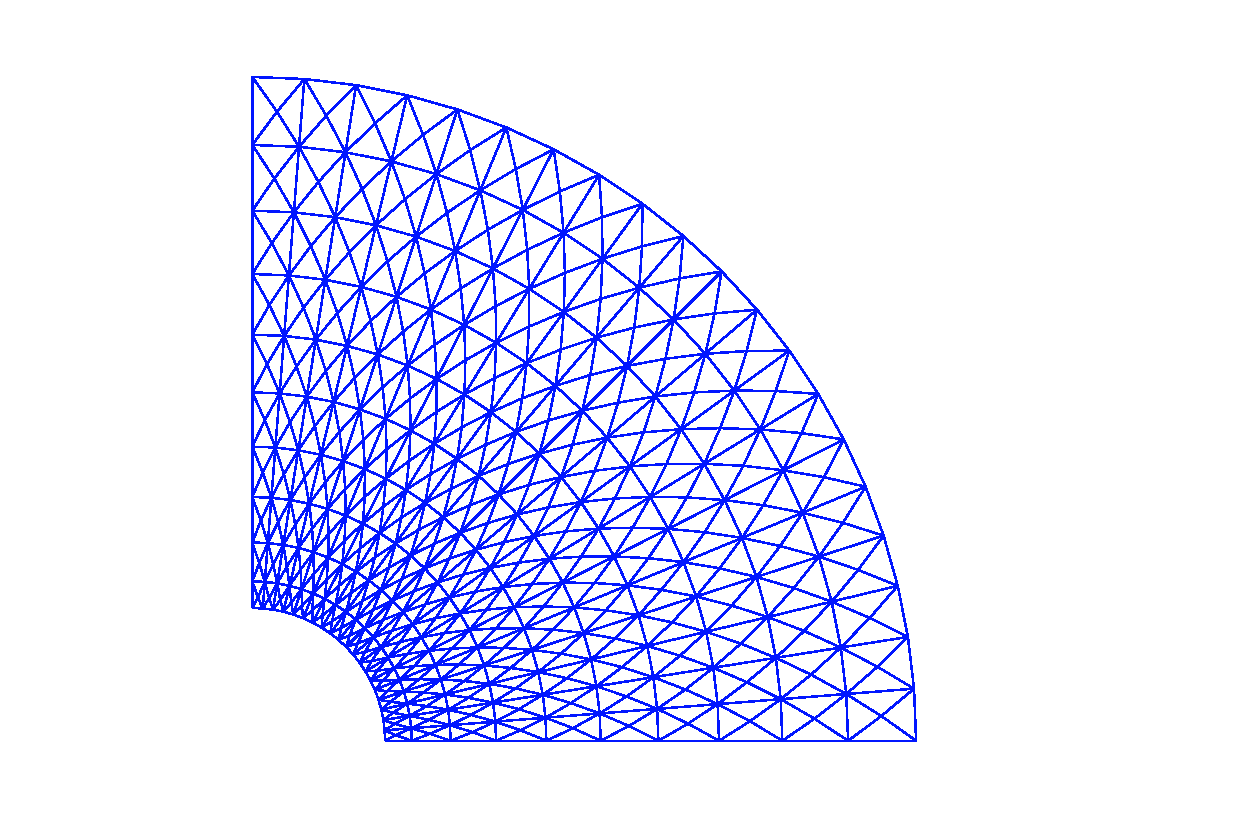
\includegraphics[width=\largefig]{chapters/langtangen/pdf/hollow_cylinder.pdf}
  \caption{A hollow cylinder generated by mapping a rectangular mesh,
  stretched toward the left side.}
\label{langtangen:mesh:transform:cyl:fig1}
\end{figure}

Setting boundary conditions in meshes created from mappings like the
one illustrated above is most conveniently done by using a mesh function
to mark parts of the boundary. The marking is easiest to perform before
the mesh is mapped since one can then conceptually work with the sides
in a pure rectangle.

\section{Handling domains with different materials}
\index{heterogeneous media}\index{multi-material domain}

Solving PDEs in domains made up of different materials is a frequently
encountered task. In \fenics, these kind of problems are handled by
defining subdomains inside the domain. The subdomains may represent
the various materials. We can thereafter define material properties
through functions, known in \fenics{} as \emph{mesh functions}, that are
piecewise constant in each subdomain.  A simple example with two materials
(subdomains) in 2D will demonstrate the basic steps in the process.

\subsection{Working with two subdomains}
\label{langtangen:possion:2D:2mat:problem}

Suppose we want to solve
\begin{equation} \label{langtangen:poisson:2D:2mat:varcoeff2}
  \nabla\cdot \left\lbrack k(x,y)\nabla u(x,y)\right\rbrack = 0,
\end{equation}
in a domain $\Omega$ consisting of two subdomains where $k$ takes on
a different value in each subdomain.
For simplicity, yet without loss of generality, we choose for the current
implementation
the domain $\Omega = [0,1]\times [0,1]$ and divide it into two equal
subdomains, as depicted in Figure~\ref{langtangen:possion:2D:2mat:fig1},
\begin{equation}
 \Omega_0 = [0, 1]\times [0,1/2],\quad \Omega_1 = [0, 1]\times (1/2,1].
\end{equation}
We define $k(x,y)=k_0$ in $\Omega_0$ and $k(x,y)=k_1$ in $\Omega_1$,
where $k_0>0$ and $k_1>0$ are given constants.  As boundary conditions,
we choose $u=0$ at $y=0$, $u=1$ at $y=1$, and $\partial u/\partial n=0$
at $x=0$ and $x=1$.  One can show that the exact solution is now given by
\begin{equation}
u(x, y) = \left\lbrace\begin{array}{ll}
\frac{2yk_1}{k_0+k_1}, & y \leqslant 1/2\\
\frac{(2y-1)k_0 + k_1}{k_0+k_1}, & y \geqslant 1/2
\end{array}\right.
\end{equation}
As long as the element boundaries coincide with the internal boundary
$y=1/2$, this piecewise linear solution should be exactly recovered
by Lagrange elements of any degree. We use this property to verify the
implementation.

\begin{figure}
% NOTE: remove everything with \SetFigFont etc. from xfig
\newcommand{\SetFigFontNFSS}[2]{}
  \centerline{
%\setlength{\unitlength}{4144sp}
\setlength{\unitlength}{2144sp}
% no blank line before begin{picture}
\begin{picture}(6372,6030)(166,-6376)
\thinlines
{\color[rgb]{0,0,0}\put(901,-5956){\vector( 0, 1){5445}}
}%
{\color[rgb]{0,0,0}\put(901,-5911){\vector( 1, 0){5625}}
}%
{\color[rgb]{0,0,0}\put(901,-2086){\line( 1, 0){3825}}
\put(4726,-2086){\line( 0,-1){3825}}
}%
{\color[rgb]{0,0,0}\put(901,-4021){\line( 1, 0){3825}}
}%
\put(6301,-6226){$x$}
\put(586,-601){$y$}
%\put(2251,-6361){$\partial u/\partial n=0$}
%\put(2251,-1861){$\partial u/\partial n=0$}
%\put(2300,-6361){$u=0$}
%\put(2300,-1861){$u=1$}
\put(2520,-6361){$u=0$}
\put(2520,-1861){$u=1$}
%\put(2431,-3211){$\Omega_1$}
%\put(2476,-5191){$\Omega_0$}
\put(2700,-3211){$\Omega_1$}
\put(2700,-5050){$\Omega_0$}
%\put(181,-4156){$u=0$}
\put(-40,-4111){$\frac{\partial u}{\partial n}=0$}
\put(4861,-4111){$\frac{\partial u}{\partial n}=0$}
\end{picture}%
  }
 \caption{Sketch of a Poisson problem with a variable coefficient that
 is constant in each of the two subdomains $\Omega_0$ and $\Omega_1$.}
\label{langtangen:possion:2D:2mat:fig1}
\end{figure}

Physically, the present problem may correspond to heat conduction, where
the heat conduction in $\Omega_1$ is ten times more efficient than in
$\Omega_0$. An alternative interpretation is flow in porous media with
two geological layers, where the layers' ability to transport the fluid
differs by a factor of 10.

\subsection{Implementation}
\label{langtangen:possion:2D:2mat:impl}

The new functionality in this subsection regards how to define
the subdomains $\Omega_0$ and $\Omega_1$. For this purpose we need to
use subclasses of class \emp{SubDomain}, \index{boundary specification
(class)} not only plain functions as we have used so far for specifying
boundaries. Consider the boundary function
\begin{python}
def boundary(x, on_boundary):
    tol = 1E-14
    return on_boundary and abs(x[0]) < tol
\end{python}
for defining the boundary $x=0$. Instead of using such a stand-alone
function, we can create an instance\footnote{The term \emph{instance}
means a Python object of a particular type (such as \emp{SubDomain},
\emp{Function}, \emp{FunctionSpace}, etc.).  Many use \emph{instance}
and \emph{object} as interchangeable terms. In other computer programming
languages one may also use the term \emph{variable} for the same thing.
We mostly use the well-known term \emph{object} in this text.} of a
subclass of \emp{SubDomain}, which implements the \emp{inside} method
as an alternative to the \emp{boundary} function:
\begin{python}
class Boundary(SubDomain):
    def inside(x, on_boundary):
        tol = 1E-14
        return on_boundary and abs(x[0]) < tol

boundary = Boundary()
bc = DirichletBC(V, Constant(0), boundary)
\end{python}

A subclass of \emp{SubDomain} with an \emp{inside} method offers
functionality for marking parts of the domain or the boundary. Now
we need to define one class for the subdomain $\Omega_0$ where $y\leqslant
1/2$ and another for the subdomain $\Omega_1$ where $y\geqslant 1/2$:
\begin{python}
class Omega0(SubDomain):
    def inside(self, x, on_boundary):
        return True if x[1] <= 0.5 else False

class Omega1(SubDomain):
    def inside(self, x, on_boundary):
        return True if x[1] >= 0.5 else False
\end{python}
Notice the use of \emp{<=} and \emp{>=} in both tests. For a cell
to belong to, e.g., $\Omega_1$, the \emp{inside} method must return
\emp{True} for all the vertices \emp{x} of the cell. So to make the cells
at the internal boundary $y=1/2$ belong to $\Omega_1$, we need the test
\emp{x[1] >= 0.5}.

The next task is to use a \emp{MeshFunction} to mark all cells in
$\Omega_0$ with the subdomain number 0 and all cells in $\Omega_1$
with the subdomain number 1.  Our convention is to number subdomains
as $0,1,2,\ldots$.
%To make programs more readable, we may introduce logical names for
%the subdomain numbers, e.g., \emp{LOWER} for no.~0 and
%\emp{UPPER} for no.~1 in our case\footnote{It is common to
%use upper case letters in name for constants that correspond to integers (known
%as \emph{enum} types).}.

A \emp{MeshFunction} is a discrete function that can be evaluated at a
set of so-called \emph{mesh entities}. Examples on mesh entities are cells,
facets, and vertices. A \emp{MeshFunction} over cells is suitable
to represent subdomains (materials), while a \emp{MeshFunction} over
facets is used to represent pieces of external or internal boundaries.
Mesh functions over vertices can be used to describe continuous fields.

Since we need to define subdomains of $\Omega$ in the present example, we
must make use of a \emp{MeshFunction} over cells. The \emp{MeshFunction}
constructor is fed with three arguments: 1) the type of value:
\emp{"int"} for integers, \emp{"uint"} for positive (unsigned) integers,
\emp{"double"} for real numbers, and \emp{"bool"} for logical values; 2)
a \emp{Mesh} object, and 3) the topological dimension of the mesh entity
in question: cells have topological dimension equal to the number of
space dimensions in the PDE problem, and facets have one dimension lower.
Alternatively, the constructor can take just a filename and initialize
the \emp{MeshFunction} from data in a file.

We start with creating a \emp{MeshFunction} whose values are non-negative
integers (\emp{"uint"}) for numbering the subdomains.  The mesh entities
of interest are the cells, which have dimension 2 in a two-dimensional
problem (1 in 1D, 3 in 3D). The appropriate code for defining the
\emp{MeshFunction} for two subdomains then reads
\begin{python}
subdomains = MeshFunction("uint", mesh, 2)
# Mark subdomains with numbers 0 and 1
subdomain0 = Omega0()
subdomain0.mark(subdomains, 0)
subdomain1 = Omega1()
subdomain1.mark(subdomains, 1)
\end{python}

Calling \emp{subdomains.values()} returns a \emp{numpy} array of the
subdomain values. That is, \emp{subdomain.values()[i]} is the subdomain
value of cell number \emp{i}. This array is used to look up the subdomain
or material number of a specific element.

We need a function \emp{k} that is constant in each subdomain $\Omega_0$
and $\Omega_1$. Since we want \emp{k} to be a finite element function,
it is natural to choose a space of functions that are constant over each
element.  The family of discontinuous Galerkin methods, in \fenics{}
denoted by \emp{"DG"}, is suitable for this purpose. Since we want
functions that are piecewise constant, the value of the degree parameter
is zero:
\begin{python}
V0 = FunctionSpace(mesh, "DG", 0)
k  = Function(V0)
\end{python}
To fill \emp{k} with the right values in each element, we loop over all
cells (the indices in \emp{subdomain.values()}), extract the corresponding
subdomain number of a cell, and assign the corresponding $k$ value to
the \emp{k.vector()} array:
\begin{python}
k_values = [1.5, 50]  # values of k in the two subdomains
for cell_no in range(len(subdomains.values())):
    subdomain_no = subdomains.values()[cell_no]
    k.vector()[cell_no] = k_values[subdomain_no]
\end{python}

Long loops in Python are known to be slow, so for large meshes it is
preferable to avoid such loops and instead use \emph{vectorized code}.
Normally this implies that the loop must be replaced by calls to
functions from the \emp{numpy} library that operate on complete arrays
(in efficient C code). The functionality we want in the present case
is to compute an array of the same size as \emp{subdomain.values()},
but where the value \emp{i} of an entry in \emp{subdomain.values()}
is replaced by \emp{k\_values[i]}.  Such an operation is carried out by
the \emp{numpy} function \emp{choose}:
\begin{python}
help = numpy.asarray(subdomains.values(), dtype=numpy.int32)
k.vector()[:] = numpy.choose(help, k_values)
\end{python}
The \emp{help} array is required since \emp{choose} cannot work with
\emp{subdomain.values()} because this array has elements of type
\emp{uint32}. We must therefore transform this array to an array
\emp{help} with standard \emp{int32} integers.

Having the \emp{k} function ready for finite element
computations, we can proceed in the normal manner
with defining essential boundary conditions, as in
Section~\ref{langtangen:poisson:multiple:Dirichlet}, and the $a(u,v)$
and $L(v)$ forms, as in Section~\ref{langtangen:possion:2D:varcoeff}.
All the details can be found in the file \emp{Poisson2D\_2mat.py}.

\subsection{Multiple Neumann, Robin, and Dirichlet conditions}
\label{langtangen:poisson:mat:neumann}
\index{Dirichlet boundary conditions}
\index{Neumann boundary conditions}
\index{Robin boundary conditions}
\index{boundary conditions}

Let us go back to the model problem from
Section~\ref{langtangen:poisson:multiple:Dirichlet} where we had both
Dirichlet and Neumann conditions.  The term \emp{v*g*ds} in the expression
for \emp{L} implies a boundary integral over the complete boundary,
or in \fenics{} terms, an integral over all exterior cell facets.
However, the contributions from the parts of the boundary where we have
Dirichlet conditions are erased when the linear system is modified by the
Dirichlet conditions.  We would like, from an efficiency point of view,
to integrate \emp{v*g*ds} only over the parts of the boundary where
we actually have Neumann conditions.  And more importantly, in other
problems one may have different Neumann conditions or other conditions
like the Robin type condition.  With the mesh function concept we can
mark different parts of the boundary and integrate over specific parts.
The same concept can also be used to treat multiple Dirichlet conditions.
The forthcoming text illustrates how this is done.

Essentially, we still stick to the model problem from
Section~\ref{langtangen:poisson:multiple:Dirichlet}, but replace the
Neumann condition at $y=0$ by a \emph{Robin condition}\footnote{The Robin
condition is most often used to model heat transfer to the surroundings
and arise naturally from Newton's cooling law.}:
\begin{equation}
 - \frac{\partial u}{\partial n} = p(u-q),
\end{equation}
where $p$ and $q$ are specified functions.  Since we have prescribed
a simple solution in our model problem, $u=1+x^2+2y^2$, we adjust
$p$ and $q$ such that the condition holds at $y=0$. This implies that
$q=1+x^2+2y^2$ and $p$ can be arbitrary (the normal derivative at $y=0$:
$\partial u/\partial n = -\partial u/\partial y = -4y=0$).

Now we have four parts of the boundary: $\Gamma_N$ which corresponds
to the upper side $y=1$, $\Gamma_R$ which corresponds to the lower part
$y=0$, $\Gamma_0$ which corresponds to the left part $x=0$, and $\Gamma_1$
which corresponds to the right part $x=1$. The complete boundary-value
problem reads
\begin{align}
  - \Delta u &= -6 \mbox{ in } \Omega,
  \label{langtangen:poisson:2D:DN3}
\\
  u &= u_L \mbox{ on } \Gamma_0,
  \label{langtangen:poisson:2D:DN3:bc1}
\\
  u &= u_R \mbox{ on } \Gamma_1,
  \label{langtangen:poisson:2D:DN3:bc2}
\\
  - \frac{\partial u}{\partial n} &= p(u-q) \mbox{ on } \Gamma_R,
  \label{langtangen:poisson:2D:DN3:bc3}
\\
  - \frac{\partial u}{\partial n} &= g \mbox{ on } \Gamma_N.
  \label{langtangen:poisson:2D:DN3:bc4}
\end{align}
The involved prescribed functions are $u_L= 1 + 2y^2$, $u_R = 2 + 2y^2$,
$q=1+x^2+2y^2$, $p$ is arbitrary, and $g=-4y$.

Integration by parts of $-\int_\Omega v\Delta u\dx$ becomes as usual
\begin{equation}
 -\int_\Omega v\Delta u \dx
= \int_\Omega\nabla u\cdot \nabla v\dx
  - \int_{\partial\Omega} \frac{\partial u}{\partial n}v\ds.
\end{equation}
The boundary integral vanishes on $\Gamma_0\cup\Gamma_1$, and we split the
parts over $\Gamma_N$ and $\Gamma_R$ since we have different conditions
at those parts:
\begin{equation}
- \int_{\partial\Omega}v \frac{\partial u}{\partial n}\ds
=
-\int_{\Gamma_N}v \frac{\partial u}{\partial n}\ds
 - \int_{\Gamma_R}v \frac{\partial u}{\partial n}\ds
= \int_{\Gamma_N}vg\ds
+ \int_{\Gamma_R}vp(u-q)\ds.
\end{equation}
The weak form then becomes
\begin{equation}
\int_{\Omega} \nabla u\cdot \nabla v \dx
+ \int_{\Gamma_N} gv\ds + \int_{\Gamma_R}p(u-q)v\ds
= \int_{\Omega} fv \dx,
\end{equation}
We want to write this weak form in the standard notation $a(u,v)=L(v)$,
which requires that we identify all integrals with \emph{both} $u$ and
$v$, and collect these in $a(u,v)$, while the remaining integrals with
$v$ and not $u$ go into $L(v)$.  The integral from the Robin condition
must of this reason be split in two parts:
\begin{equation}
 \int_{\Gamma_R}p(u-q)v\ds
= \int_{\Gamma_R}puv\ds - \int_{\Gamma_R}pqv\ds.
\end{equation}
We then have
\begin{align}
  a(u, v) &= \int_{\Omega} \nabla u\cdot \nabla v \dx
    + \int_{\Gamma_R}puv\ds,
  \label{langtangen:poisson:2D:DN3:var:a}
\\
  L(v) &= \int_{\Omega} fv \dx - \int_{\Gamma_N} g v\ds + \int_{\Gamma_R}pqv\ds.
  \label{langtangen:poisson:2D:DN3:var:L}
\end{align}

A natural starting point for implementation is the \emp{Poisson2D\_DN2.py}
program, which we now copy to \emp{Poisson2D\_DNR.py}.  The new aspects
are
\begin{enumerate}
\item definition of a mesh function over the boundary,
\item marking each side as a subdomain, using the mesh function,
\item splitting a boundary integral into parts.
\end{enumerate}
%%
Task 1 makes use of the \emp{MeshFunction} object, but contrary to
Section~\ref{langtangen:possion:2D:2mat:impl}, this is not a function
over cells, but a function over cell facets. The topological dimension of
cell facets is one lower than the cell interiors, so in a two-dimensional
problem the dimension becomes 1. In general, the facet dimension is given
as \emp{mesh.topology().dim()-1}, which we use in the code for ease of
direct reuse in other problems.  The construction of a \emp{MeshFunction}
object to mark boundary parts now reads
\begin{python}
boundary_parts = \
  MeshFunction("uint", mesh, mesh.topology().dim()-1)
\end{python}
As in Section~\ref{langtangen:possion:2D:2mat:impl} we use a
subclass of \emp{SubDomain} to identify the various parts of the mesh
function. Problems with domains of more complicated geometries may set
the mesh function for marking boundaries as part of the mesh generation.
In our case, the $y=0$ boundary can be marked by
\begin{python}
class LowerRobinBoundary(SubDomain):
    def inside(self, x, on_boundary):
        tol = 1E-14   # tolerance for coordinate comparisons
        return on_boundary and abs(x[1]) < tol

Gamma_R = LowerRobinBoundary()
Gamma_R.mark(boundary_parts, 0)
\end{python}
The code for the $y=1$ boundary is similar and is seen in
\emp{Poisson2D\_DNR.py}.

The Dirichlet boundaries are marked similarly, using subdomain number
2 for $\Gamma_0$ and 3 for~$\Gamma_1$:
\begin{python}
class LeftBoundary(SubDomain):
    def inside(self, x, on_boundary):
        tol = 1E-14   # tolerance for coordinate comparisons
        return on_boundary and abs(x[0]) < tol

Gamma_0 = LeftBoundary()
Gamma_0.mark(boundary_parts, 2)

class RightBoundary(SubDomain):
    def inside(self, x, on_boundary):
        tol = 1E-14   # tolerance for coordinate comparisons
        return on_boundary and abs(x[0] - 1) < tol

Gamma_1 = RightBoundary()
Gamma_1.mark(boundary_parts, 3)
\end{python}
Specifying the \emp{DirichletBC} objects may now make use of the mesh
function (instead of a \emp{SubDomain} subclass object) and an indicator
for which subdomain each condition should be applied to:
\begin{python}
u_L = Expression("1 + 2*x[1]*x[1]")
u_R = Expression("2 + 2*x[1]*x[1]")
bc = [DirichletBC(V, u_L, boundary_parts, 2),
      DirichletBC(V, u_R, boundary_parts, 3)]
\end{python}

Some functions need to be defined before we can go on with the \emp{a}
and \emp{L} of the variational problem:
\begin{python}
g = Expression("-4*x[1]")
q = Expression("1 + x[0]*x[0] + 2*x[1]*x[1]")
p = Constant(100)  # arbitrary function can go here
u = TrialFunction(V)
v = TestFunction(V)
f = Constant(-6.0)
\end{python}

The new aspect of the variational problem is the two distinct boundary
integrals.  Having a mesh function over exterior cell facets (our
\emp{boundary\_parts} object), where subdomains (boundary parts) are
numbered as $0,1,2,\ldots$, the special symbol \emp{ds(0)} implies
integration over subdomain (part) 0, \emp{ds(1)} denotes integration
over subdomain (part) 1, and so on.  The idea of multiple \emp{ds}-type
objects generalizes to volume integrals too: \emp{dx(0)}, \emp{dx(1)},
etc., are used to integrate over subdomain 0, 1, etc., inside $\Omega$.

The variational problem can be defined as
\begin{python}
a = inner(grad(u), grad(v))*dx + p*u*v*ds(0)
L = f*v*dx - g*v*ds(1) + p*q*v*ds(0)
\end{python}
For the \emp{ds(0)} and \emp{ds(1)} symbols to work we must obviously
connect them (or \emp{a} and \emp{L}) to the mesh function marking
parts of the boundary. This is done by a certain keyword argument to
the \emp{assemble} function:
\begin{python}
A = assemble(a, exterior_facet_domains=boundary_parts)
b = assemble(L, exterior_facet_domains=boundary_parts)
\end{python}
Then essential boundary conditions are enforced, and the system can be
solved in the usual way:
\begin{python}
for condition in bc: condition.apply(A, b)
u = Function(V)
solve(A, u.vector(), b)
\end{python}

At the time of this writing, it is not possible to perform integrals over
different parts of the domain or boundary using the \emp{assemble\_system}
function or the \emp{VariationalProblem} object.

\section{More examples}

Many more topics could be treated in a \fenics{} tutorial, e.g., how
to solve systems of PDEs, how to work with mixed finite element
methods, how to create more complicated meshes and mark boundaries,
and how to create more advanced visualizations.  However, to limit the
size of this tutorial, the examples end here.  There are, fortunately,
a rich set of FEniCS demos.  The FEniCS documentation explains a
collection of PDE solvers in detail: the Poisson equation, the mixed
formulation for the Poisson equation, the Biharmonic equation, the
equations of hyperelasticity, the Cahn-Hilliard equation, and the
incompressible Navier--Stokes equations.  Both Python and C++ versions
of these solvers are explained.  An eigenvalue solver is also
documented.  In the \emp{dolfin/demo} directory of the DOLFIN source
code tree you can find programs for these and many other examples,
including the advection-diffusion equation, the equations of
elastodynamics, a reaction-diffusion equation, various finite element
methods for the Stokes problem, discontinuous Galerkin methods for the
Poisson and advection-diffusion equations, and an eigenvalue problem
arising from electromagnetic waveguide problem with \nedelec{}
elements.  There are also numerous demos on how to apply various
functionality in FEniCS, e.g., mesh refinement and error control,
moving meshes (for ALE methods), computing functionals over subsets of
the mesh (such as lift and drag on bodies in flow), and creating
separate subdomain meshes from a parent mesh.

The project CBC.Solve (\emp{https://launchpad.net/cbc.solve}) offers
more complete PDE solvers for the Navier--Stokes equations
(Chapter~\ref{chap:selim}), the equations of hyperelasticity
(Chapter~\ref{chap:narayanan}), fluid--structure interaction
(Chapter~\ref{chap:selim}), viscous mantle flow
(Chapter~\ref{chap:vynnytska}), and the bidomain model of
electrophysiology.  Another project, CBC.RANS
(\emp{https://launchpad.net/cbc.rans}), offers an environment for very
flexible and easy implementation of systems of nonlinear PDEs in
general, and a collection of Navier--Stokes solvers and turbulence
models in particular \citet{Mortensen2011,Mortensen2011b}. For example,
CBC.RANS contains an elliptic relaxation model for turbulent flow
involving 18 nonlinear PDEs. FEniCS proved to be an ideal environment
for implementing such complicated PDE models.

\section{Miscellaneous topics}


\subsection{Glossary}

Below we explain some key terms used in this tutorial.
%
\begin{trivlist}
  \item[\fenics:] name of a software suite composed of many individual
  software components (see \emp{fenicsproject.org}). Some components are
  DOLFIN and Viper, explicitly referred to in this tutorial. Others are
  FFC and FIAT, heavily used by the programs appearing in this tutorial,
  but never explicitly used from the programs.

  \item[DOLFIN:] a \fenics{} component, more precisely a C++ library,
  with a Python interface, for performing important actions in finite
  element programs. DOLFIN makes use of many other \fenics{} components
  and many external software packages.

  \item[Viper:] a \fenics{} component for quick visualization of finite
  element meshes and solutions.

  \item[UFL:] a \fenics{} component implementing the \emph{unified
  form language} for specifying finite element forms in \fenics{}
  programs.  The definition of the forms, typically called
  \emp{a} and \emp{L} in this tutorial, must have legal UFL
  syntax. The same applies to the definition of functionals (see
  Section~\ref{langtangen:poisson1:functionals}).

  \item[Class (Python):] a programming construction for creating objects
  containing a set of variables and functions. Most types of \fenics{}
  objects are defined through the class concept.

  \item[Instance (Python):] an object of a particular type, where the type
  is implemented as a class. For instance, \emp{mesh = UnitInterval(10)}
  creates an instance of class \emp{UnitInterval}, which is reached by
  the name \emp{mesh}. (Class \emp{UnitInterval} is actually just an
  interface to a corresponding C++ class in the DOLFIN C++ library.)

  \item[Class method (Python):] a function in a class, reached by dot
  notation: \emp{instance\_name.method\_name}.

  \item[\emp{self} parameter (Python):] required first parameter in class
  methods, representing a particular object of the class.\index{self} Used
  in method definitions, but never in calls to a method.  For example,
  if \emp{method(self, x)} is the definition of \emp{method} in a class
  \emp{Y}, \emp{method} is called as \emp{y.method(x)}, where \emp{y}
  is an instance of class \emp{X}.  In a call like \emp{y.method(x)},
  \emp{method} is invoked with \emp{self=y}.

  \item[Class attribute (Python):] a variable in a class, reached by
  dot notation: \emp{instance\_name.attribute\_name}.
\end{trivlist}

\subsection{Overview of objects and functions}

Most classes in \fenics{} have an explanation of the purpose and usage
that can be seen by using the general documentation command \emp{pydoc}
for Python objects. You can type\index{pydoc}
\begin{progoutput}
pydoc dolfin.X
\end{progoutput}
%
to look up documentation of a Python class \emp{X} from the DOLFIN
library (\emp{X} can be \emp{UnitSquare}, \emp{Function}, \emp{Viper},
etc.). Below is an overview of the most important classes and functions
in \fenics{} programs, in the order they typically appear within
programs.
%
\begin{trivlist}
  \item[\emp{UnitSquare(nx, ny)}:] generate mesh over the unit square
  $[0,1]\times [0,1]$ using \emp{nx} divisions in $x$ direction and
  \emp{ny} divisions in $y$ direction. Each of the \emp{nx*ny} squares
  are divided into two cells of triangular shape.

  \item[\emp{UnitInterval}, \emp{UnitCube}, \emp{UnitCircle},
  \emp{UnitSphere}, \emp{Interval}, \emp{Rectangle}, and \emp{Box}:]
  generate mesh over domains of simple geometric shape, see
  Section~\ref{langtangen:prepro}.

  \item[\emp{FunctionSpace(mesh, element\_type, degree)}:] a
  function space defined over a mesh, with a given element type (e.g.,
  \emp{"Lagrange"} or \emp{"DG"}), with basis functions as polynomials
  of a specified degree.

  \item[\emp{Expression(formula)}:] a scalar- or vector-valued function,
  given as a mathematical expression \emp{formula} (string) written in
  C++ syntax.

  \item[\emp{Function(V)}:] a scalar- or vector-valued finite element
  field in the function space \emp{V}. If \emp{V} is a \emp{FunctionSpace}
  object, \emp{Function(V)} becomes a scalar field, and with \emp{V}
  as a \emp{VectorFunctionSpace} object, \emp{Function(V)} becomes a
  vector field.

  \item[\emp{SubDomain}:] class for defining a subdomain, either
  a part of the boundary, an internal boundary, or a part of
  the domain.  The programmer must subclass \emp{SubDomain} and
  implement the \emp{inside(self, x, on\_boundary)} function (see
  Section~\ref{langtangen:poisson1:impl}) for telling whether a point
  \emp{x} is inside the subdomain or not.

  \item[\emp{Mesh}:] class for representing a finite element mesh,
  consisting of cells, vertices, and optionally faces, edges, and facets.

  \item[\emp{MeshFunction}:] tool for marking parts of the domain or
  the boundary.  Used for variable coefficients (``material properties'',
  see Section~\ref{langtangen:possion:2D:2mat:problem}) or for boundary
  conditions (see Section~\ref{langtangen:poisson:mat:neumann}).

  \item[\emp{DirichletBC(V, value, where)}:] specification of Dirichlet
  (essential) boundary conditions via a function space \emp{V}, a
  function \emp{value(x)} for computing the value of the condition at
  a point \emp{x}, and a specification \emp{where} of the boundary,
  either as a \emp{SubDomain} subclass instance, a plain function, or
  as a \emp{MeshFunction} instance.  In the latter case, a 4th argument
  is provided to describe which subdomain number that describes the
  relevant boundary.

  \item[\emp{TrialFunction(V)}:] define a trial function on a space
  \emp{V} to be used in a variational form to represent the unknown in
  a finite element problem.

  \item[\emp{TestFunction(V)}:] define a test function on a space \emp{V}
  to be used in a variational form.

  \item[\emp{assemble(X)}:] assemble a matrix, a right-hand side, or a
  functional, given a from \emp{X} written with UFL syntax.

  \item[\emp{assemble\_system(a, L, bc)}:] assemble the matrix and the
  right-hand side from a bilinear (\emp{a}) and linear (\emp{L}) form
  written with UFL syntax. The \emp{bc} parameter holds one or more
  \emp{DirichletBC} objects.

  \item[\emp{VariationalProblem(a, L, bc)}:] define and solve a
  variational problem, given a bilinear (\emp{a}) and linear (\emp{L})
  form, written with UFL syntax, and one or more \emp{DirichletBC}
  objects stored in \emp{bc}.

  \item[\emp{solve(A, U, b)}:] solve a linear system with \emp{A}
  as coefficient matrix (\emp{Matrix} object), \emp{U} as unknown
  (\emp{Vector} object), and \emp{b} as right-hand side (\emp{Vector}
  object).  Usually, \emp{U} is replaced by \emp{u.vector()}, where
  \emp{u} is a \emp{Function} object representing the unknown finite
  element function of the problem, while \emp{A} and \emp{b} are computed
  by calls to \emp{assemble} or \emp{assemble\_system}.

  \item[\emp{plot(q)}:] quick visualization of a mesh, function, or mesh
  function \emp{q}, using the Viper component in \fenics{}.

  \item[\emp{interpolate(func, V)}:] interpolate a formula or finite
  element function \emp{func} onto the function space \emp{V}.

  \item[\emp{project(func, V)}:] project a formula or finite element
  function \emp{func} onto the function space \emp{V}.
\end{trivlist}

\subsection{Installing \fenics}
\label{langtangen:app:install}
\label{installing FEniCS}

The \fenics{} software components are available for Linux, Windows and
Mac OS X platforms. Detailed information on how to get \fenics{} running
on such machines are available at the \emp{fenicsproject.org} website.
Here are just some quick descriptions and recommendations by the author.

To make the installation of \fenics{} as painless and reliable
as possible, the reader is strongly recommended to use Ubuntu
Linux\footnote{Even though Mac users now can get \fenics{} by a
  one-click install, I recommend using Ubuntu on Mac, unless you have
  high Unix competence and much experience with compiling and linking C++
  libraries on Mac OS X.}. Any standard PC can easily be equipped
with Ubuntu Linux, which may live side by side with either Windows
or Mac OS X or another Linux installation.  Basically, you download
Ubuntu from \url{http://www.ubuntu.com/getubuntu/download}, burn the
file on a CD, reboot the machine with the CD, and answer some usually
straightforward questions (if necessary). The graphical user interface
(GUI) of Ubuntu is quite similar to both Windows 7 and Mac OS X, but to
be efficient when doing science with \fenics{} this author recommends
to run programs in a terminal window and write them in a text editor
like Emacs or Vim. You can employ integrated development environment
such as Eclipse, but intensive \fenics{} developers and users tend to
find terminal windows and plain text editors more user friendly.

Instead of making it possible to boot your machine with the Linux
Ubuntu operating system, you can run Ubuntu in a separate window in
your existing operation system. On Mac, you can use the VirtualBox
software available from \emp{http://www.virtualbox.org} to run
Ubuntu. On Windows, Wubi makes a tool that automatically installs
Ubuntu on the machine. Just give a user~name and password for the
Ubuntu installation, and Wubi performs the rest. You can also use
VirtualBox on Windows machines.

Once the Ubuntu window is up and running, \fenics{} is painlessly
installed by
\vspace{4pt}
\begin{bash}
sudo apt-get install fenics
\end{bash}
Sometimes the \fenics{} software in a standard Ubuntu installation lacks
some recent features and bug fixes. Visiting \emp{fenicsproject.org}
and copying just five Unix commands is all you have to do to install a
newer version of the software.

\subsection{Books on the finite element method}
\label{langtangen:appendix:books}

There are a large number of books on the finite element method.  The books
typically fall in either of two categories: the abstract mathematical
version of the method and the engineering ``structural analysis''
formulation. \fenics{} builds heavily on concepts in the abstract
mathematical exposition.  An easy-to-read book, which provides a good
general background for using \fenics, is \citet{Gockenbach2006}. The
book~\citet{DoneaHuerta2003} has a similar style, but aims at readers
with interest in fluid flow problems. \citet{Hughes1987} is also highly
recommended, especially for those interested in solid mechanics and heat
transfer applications.

Readers with background in the engineering ``structural analysis''
version of the finite element method may find \citet{Bickford1994}
as an attractive bridge over to the abstract mathematical formulation
that \fenics{} builds upon.  Those who have a weak background in
differential equations in general should consult a more fundamental
book, and \citet{ErikssonEstepHansboEtAl1996} is a very good
choice. On the other hand, \fenics{} users with a strong background in
mathematics and interest in the mathematical properties of the finite
element method, will appreciate the texts \citet{BrennerScott2008},
\citet{Braess2007}, \citet{ErnGuermond2004}, \citet{QuarteroniValli2008},
or \citet{Ciarlet2002}.

\subsection{Books on Python}
\label{langtangen:appendix:pybooks}

Two very popular introductory books on Python are ``Learning Python''
\citep{Lutz2007} and ``Practical Python'' \citep{Hetland2002}.
More advanced and comprehensive books include ``Programming Python''
\citep{Lutz2006}, and ``Python Cookbook'' \citep{MartelliAscher2005}
and ``Python in a Nutshell'' \citep{Martelli2006}.  The web
page \emp{http://wiki.python.org/moin/PythonBooks} lists
numerous additional books.  Very few texts teach Python in
a mathematical and numerical context, but the references
\citet{Langtangen2008,Langtangen20011,Kiusalaas2010} are exceptions.

\subsection{User-defined functions}
\label{langtangen:app:cpp:functions}

%outdated:
%User-defined functions are implemented as a \emp{Function} object.
%There are several ways of constructing such objects, such as
%\begin{itemize}
%\item a string containing a mathematical expression,
%\item a subclass of \emp{Function} in Python,
%\item a subclass of \emp{Function} in C++,
%\item a set of degrees of freedom of a finite element function.
%\end{itemize}
%Writing \emp{pydoc dolfin.Function} gives a documentation of the various
%techniques.

When defining a function in terms of a mathematical expression inside
a string formula, e.g.,
\begin{python}
myfunc = Expression("sin(x[0])*cos(x[1])")
\end{python}
the expression contained in the first argument will be turned into a C++
function and compiled to gain efficiency. Therefore, the syntax used
in the expression must be valid C++ syntax.  Most Python syntax for
mathematical expressions are also valid C++ syntax, but power expressions
make an exception: \emp{p**a} must be written as \emp{pow(p,a)}
in C++ (this is also an alternative Python syntax).  The following
mathematical functions can be used directly in C++ expressions when
defining \emp{Expression} objects: \emp{cos}, \emp{sin}, \emp{tan},
\emp{acos}, \emp{asin}, \emp{atan}, \emp{atan2}, \emp{cosh}, \emp{sinh},
\emp{tanh}, \emp{exp}, \emp{frexp}, \emp{ldexp}, \emp{log}, \emp{log10},
\emp{modf}, \emp{pow}, \emp{sqrt}, \emp{ceil}, \emp{fabs}, \emp{floor},
and \emp{fmod}.  Moreover, the number $\pi$ is available as the symbol
\emp{pi}.  All the listed functions are taken from the \emp{cmath} C++
header file, and one may hence consult documentation of \emp{cmath}
for more information on the various functions.

\paragraph{Acknowledgments.}

The author is very thankful to Johan Hake, Anders Logg, Kent-Andre
Mardal, and Kristian Valen-Sendstad for promptly answering all my
questions about \fenics{} functionality and for implementing all my
requests. I will in particular thank Professor Douglas Arnold for very
valuable feedback on the text. {\O}ystein S{\o}rensen pointed out a lot
of typos and contributed with many helpful comments.  Many errors and
typos were also reported by Mauricio Angeles, Ida Dr{\o}sdal, and Hans
Ekkehard Plesser. Ekkehard Ellmann as well as two anonymous reviewers
provided a series of suggestions and improvements.
